\documentclass[12pt,a4paper]{article}
\usepackage[utf8]{inputenc}
\usepackage{amsmath}
\usepackage{amsfonts}
\usepackage{amssymb}
\usepackage{graphicx}
\usepackage{subcaption}
\usepackage{float}
\usepackage{multirow}
\usepackage{rotating}

\author{Team Gamma \\ {\small Ajda Frankovič, Martin Preradović, Niki Bizjak}}
\title{Colour recognition}
\date{}
\begin{document}
	
	\maketitle
	
	For our second task we were training a classifier to recognize six different colours - red, green, blue, yellow, white and black. We divided the task into three parts. 

	\begin{enumerate}
		\item Obtaining data for training and testing set
		\item Training different classifiers
		\item Evaluating the performance of trained classifiers
	\end{enumerate}
		
	\section{Preparing training and testing data}

	The first, most time consuming part was obtaining training and testing sets - images of unicolour objects under different conditions (illumination and viewing angle). After the training and testing data sets were created, each image had to be labelled and cropped so it only contained the object of interest. \\

	\subsection{Taking photos}
	
	We chose to take two groups of photos. For the first set of images we took photos of unicolour circles under different viewing angles and under different light conditions. We played with not just the light intensity but also it's colour as can be seen in the photos below. We obtained around 200 images of this kind. For simplicity, we used a simple unicolour circles of different colours. The circular shape was selected because it is easy to detect and cropping can be done automatically using Hough transformation method. \\
	
	Below we present a subset of those images. It can be seen that some of the pictures were taken in dark environment, some were taken under blue / yellow lights, we also tried using very high ISO to simulate grain, etc. We also included multiple different shades of the same colour. This is important because the 3D objects that our robot will encounter won't be of an uniform colour. Some parts of the objects will be darker, some lighter and the overall shade will change depending on which direction the robot will see the object from.

	\begin{figure}[H]
		\centering
		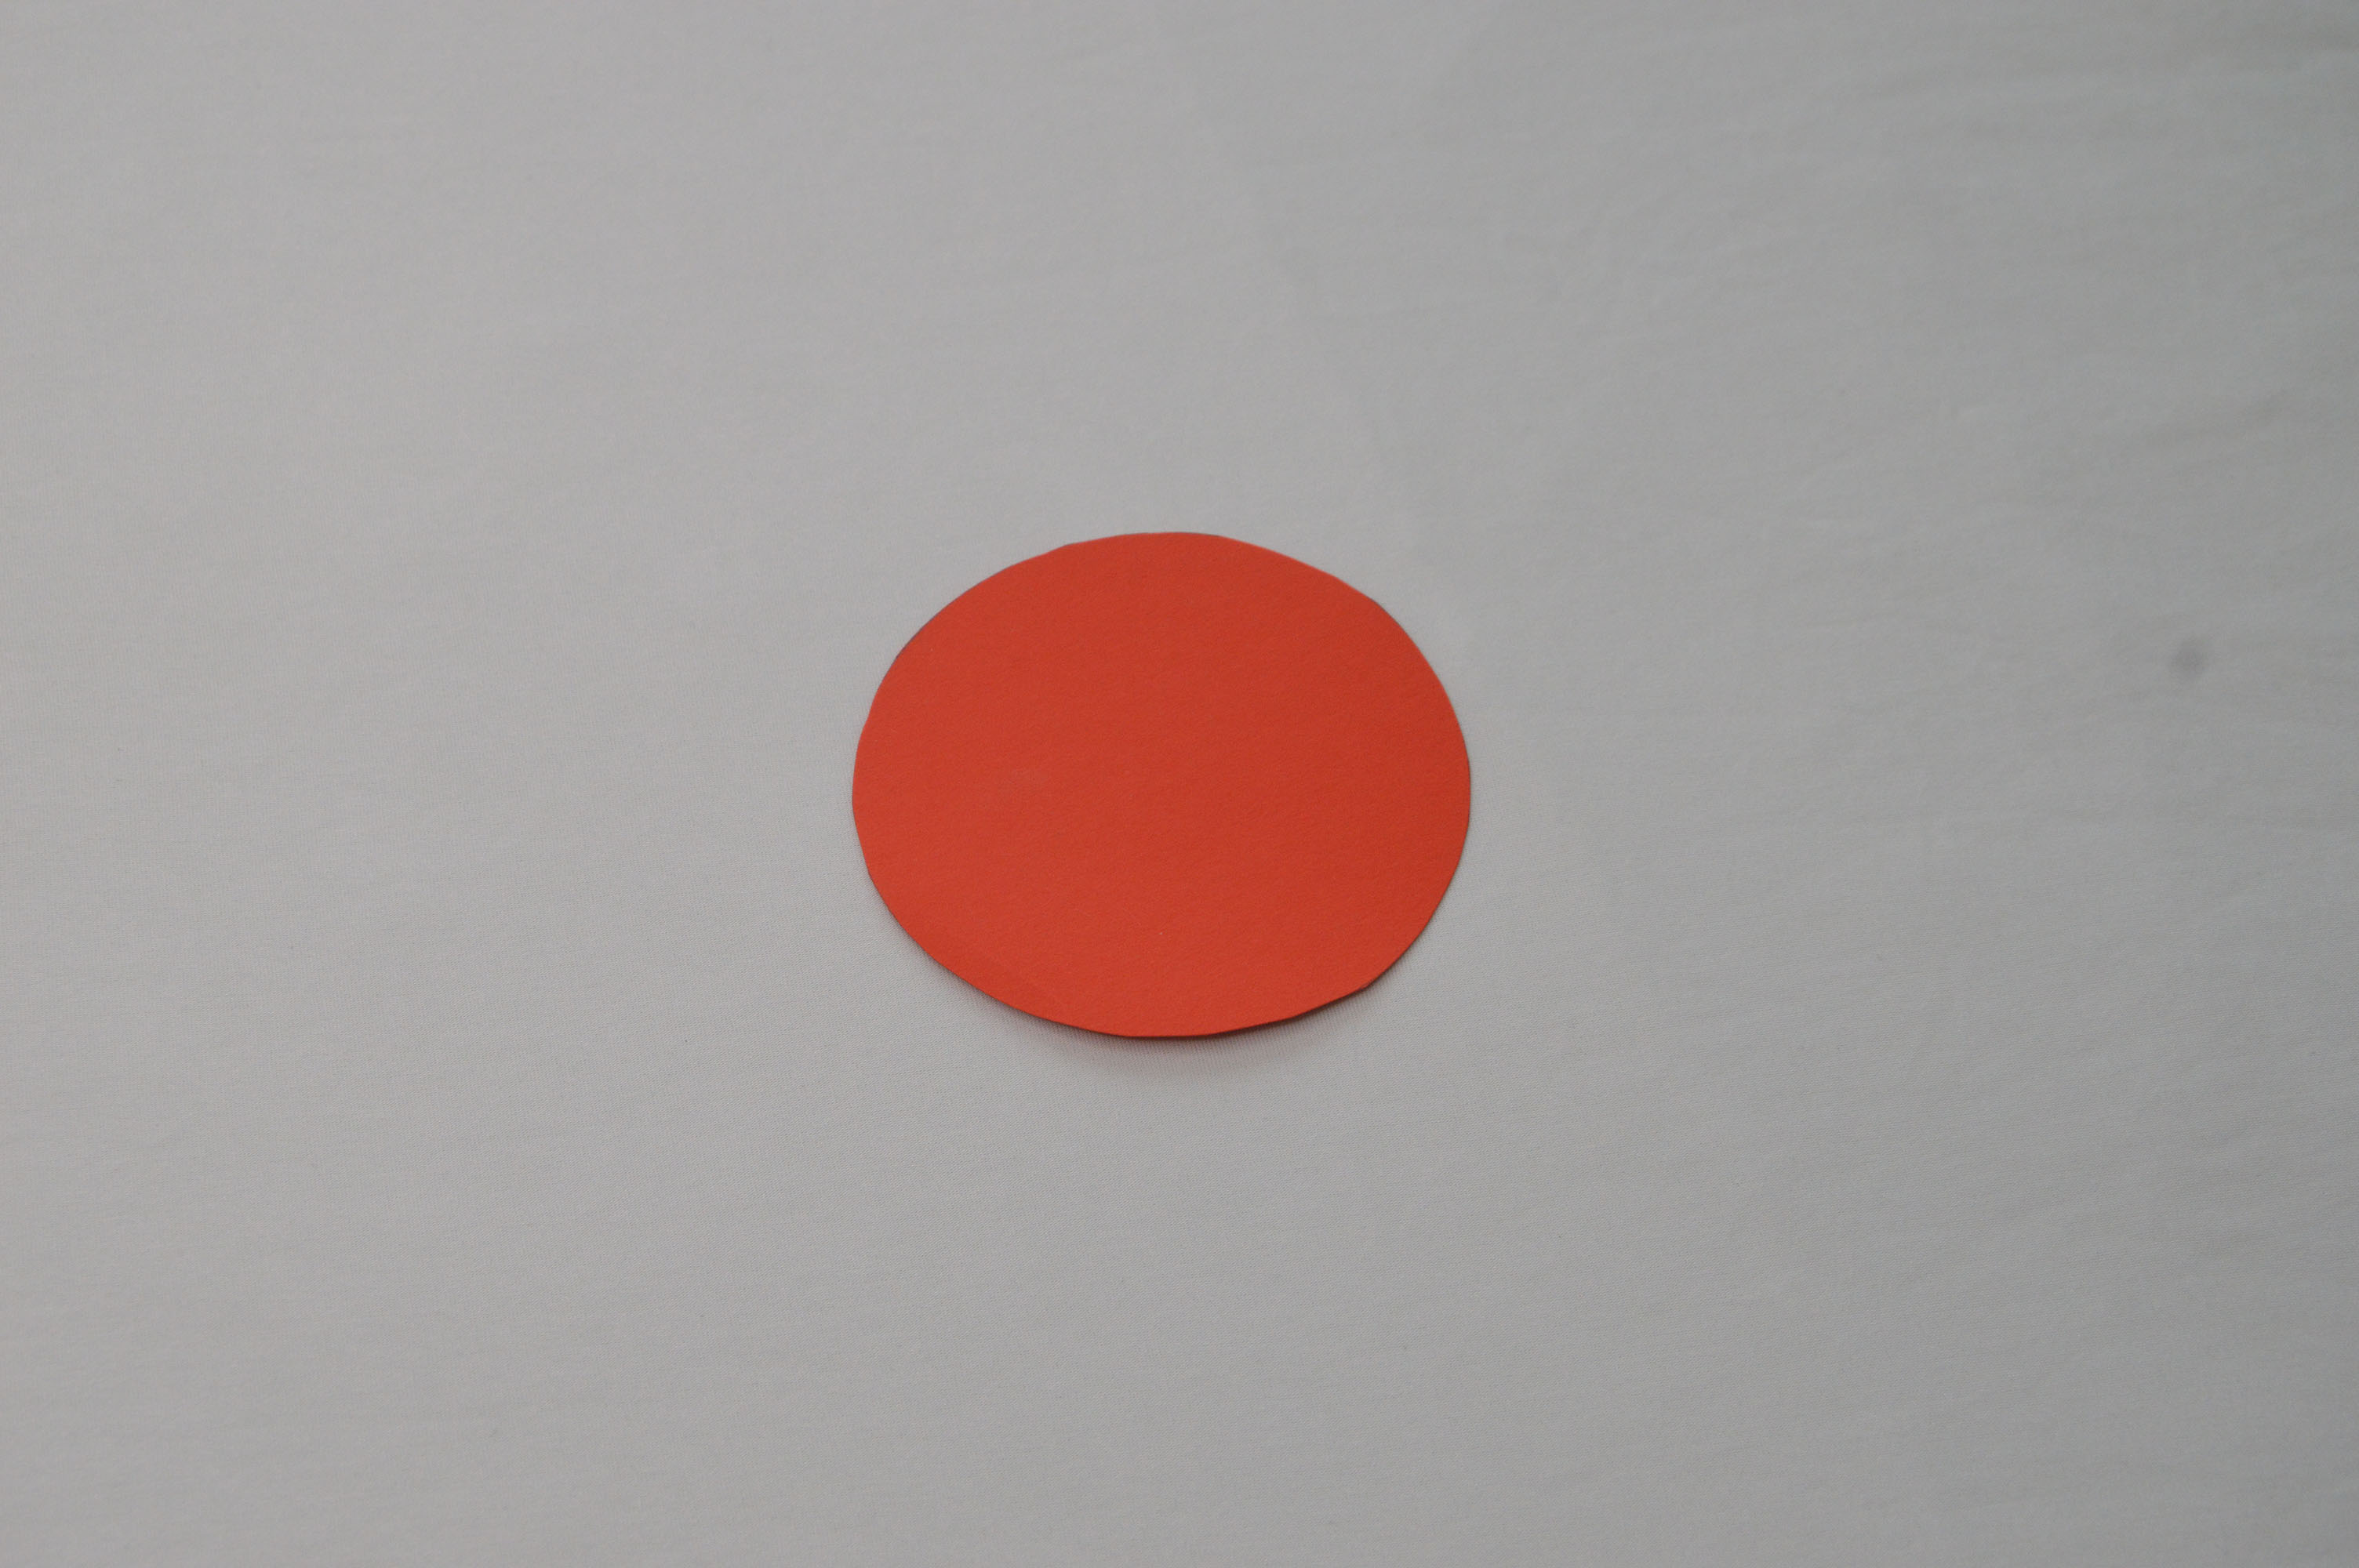
\includegraphics[width=.20\linewidth]{images/train01.jpg}
		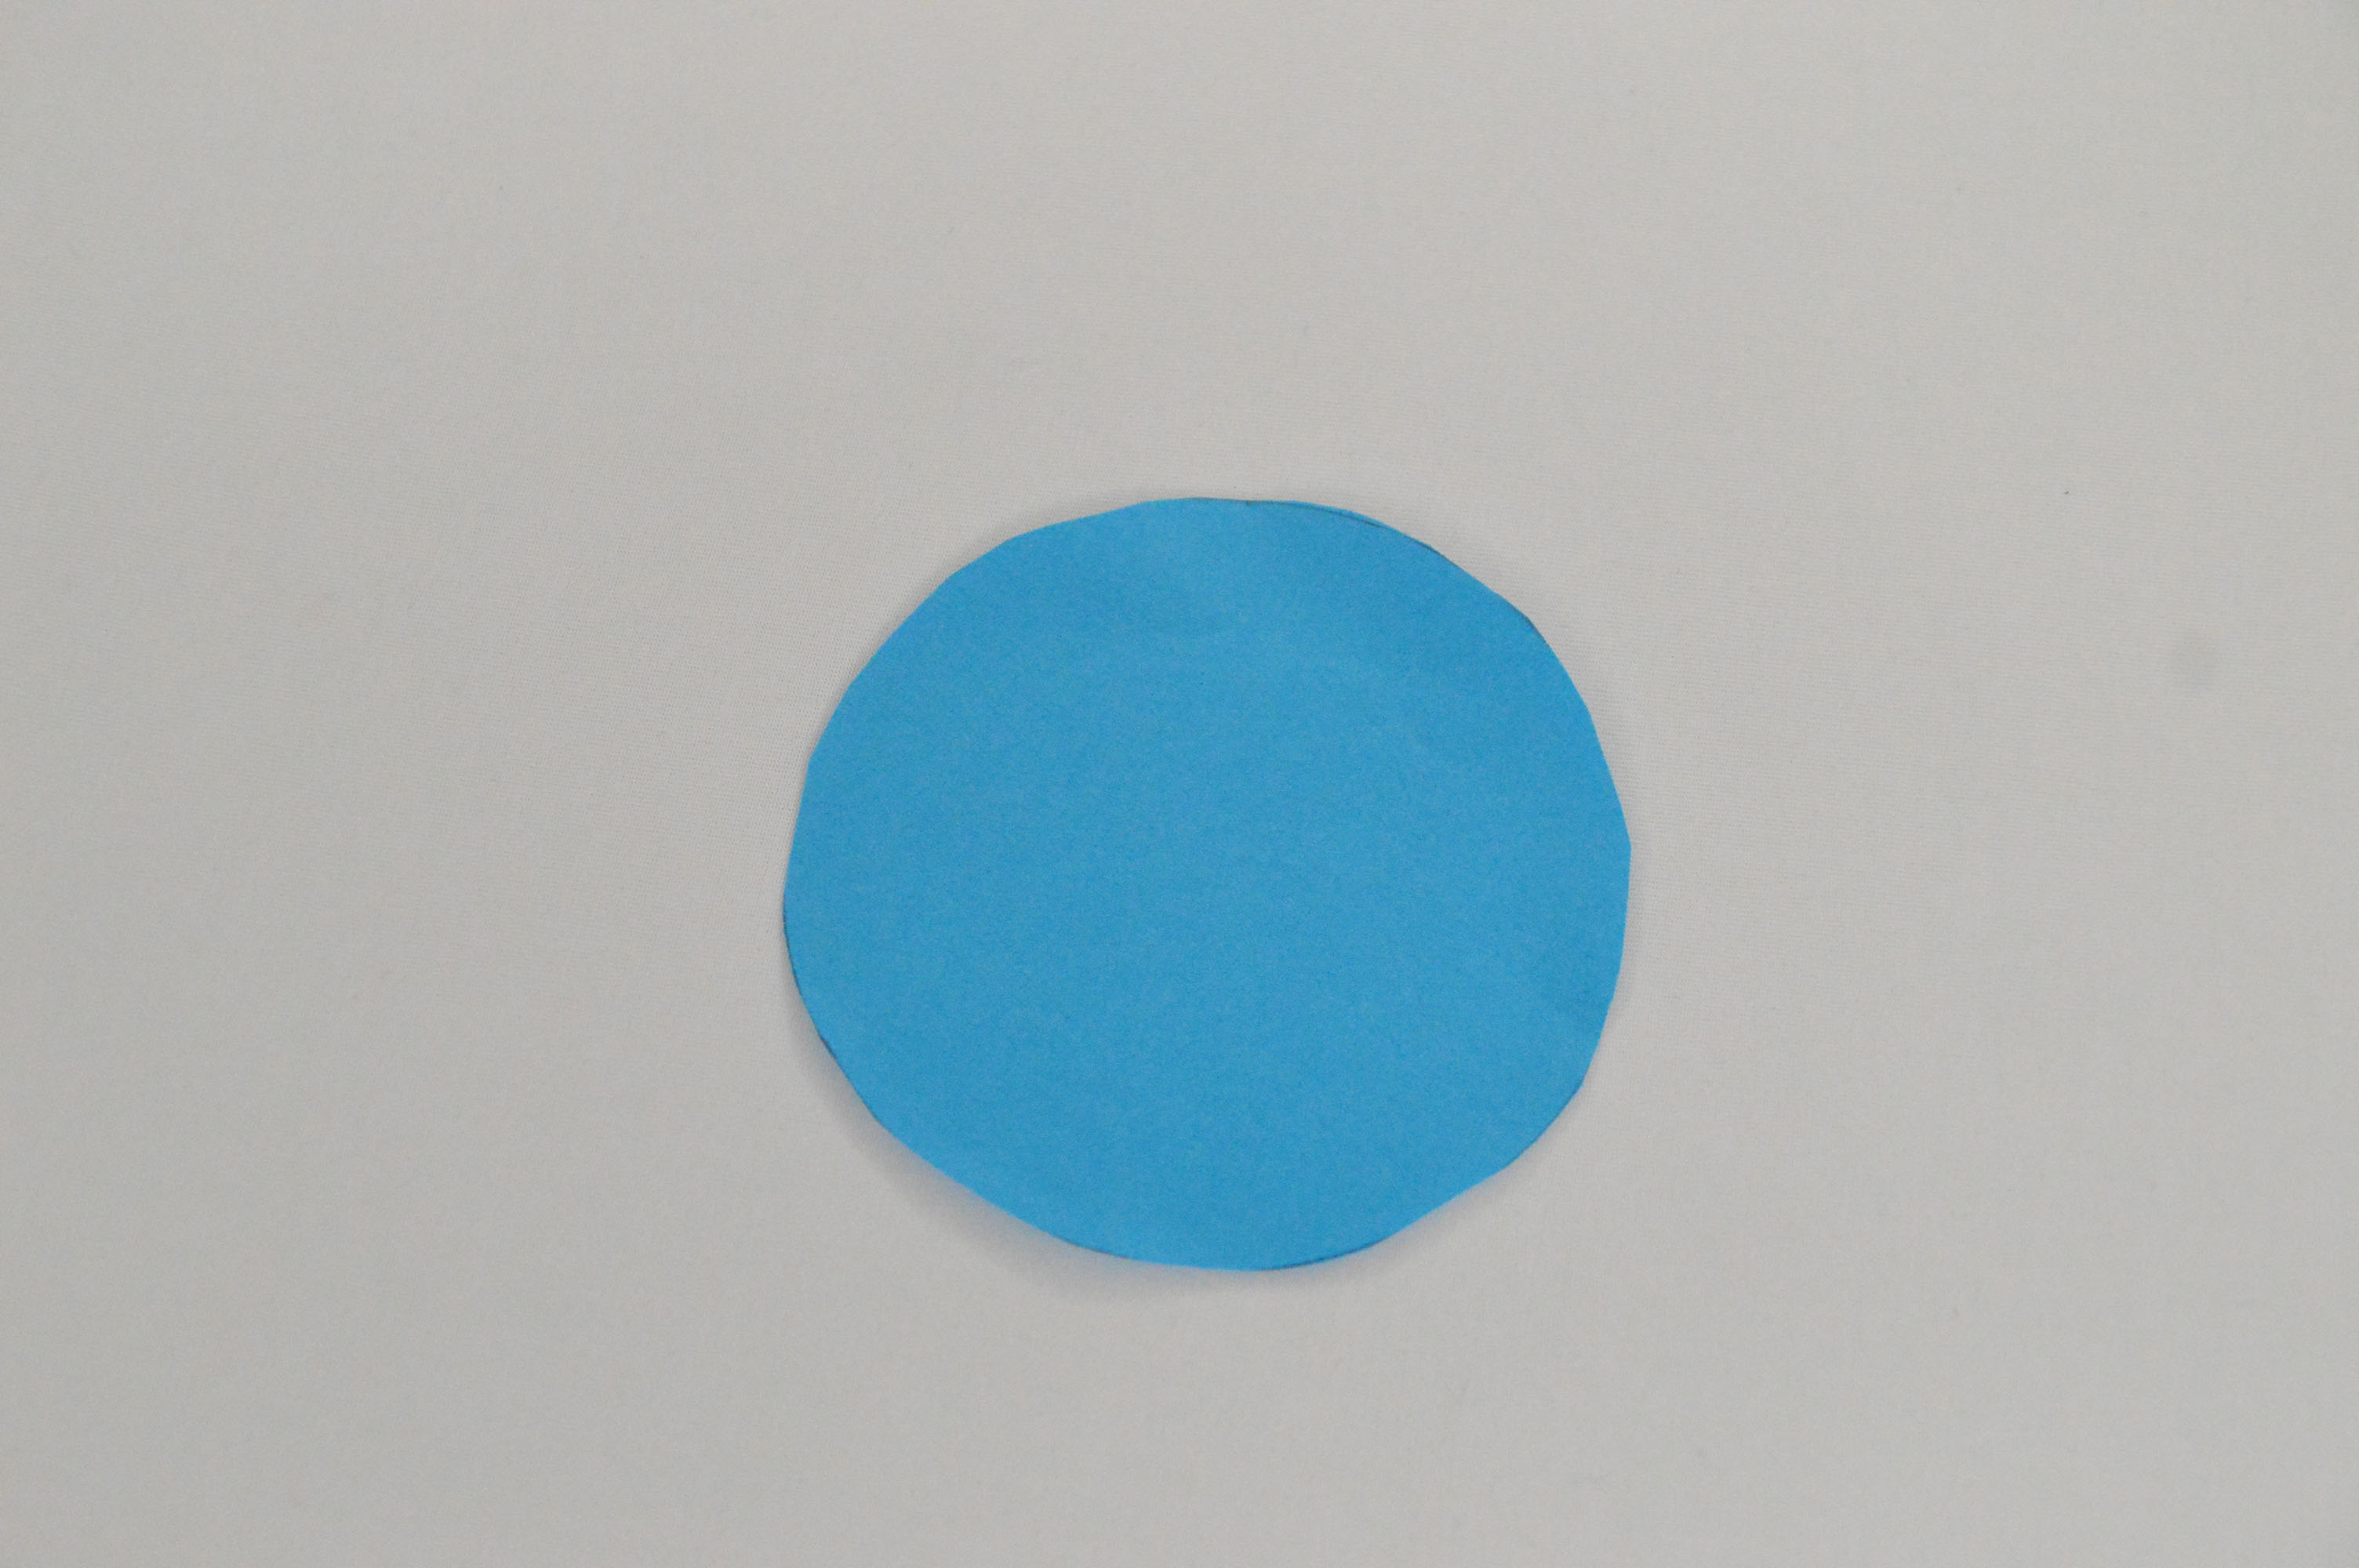
\includegraphics[width=.20\linewidth]{images/train02.jpg}
		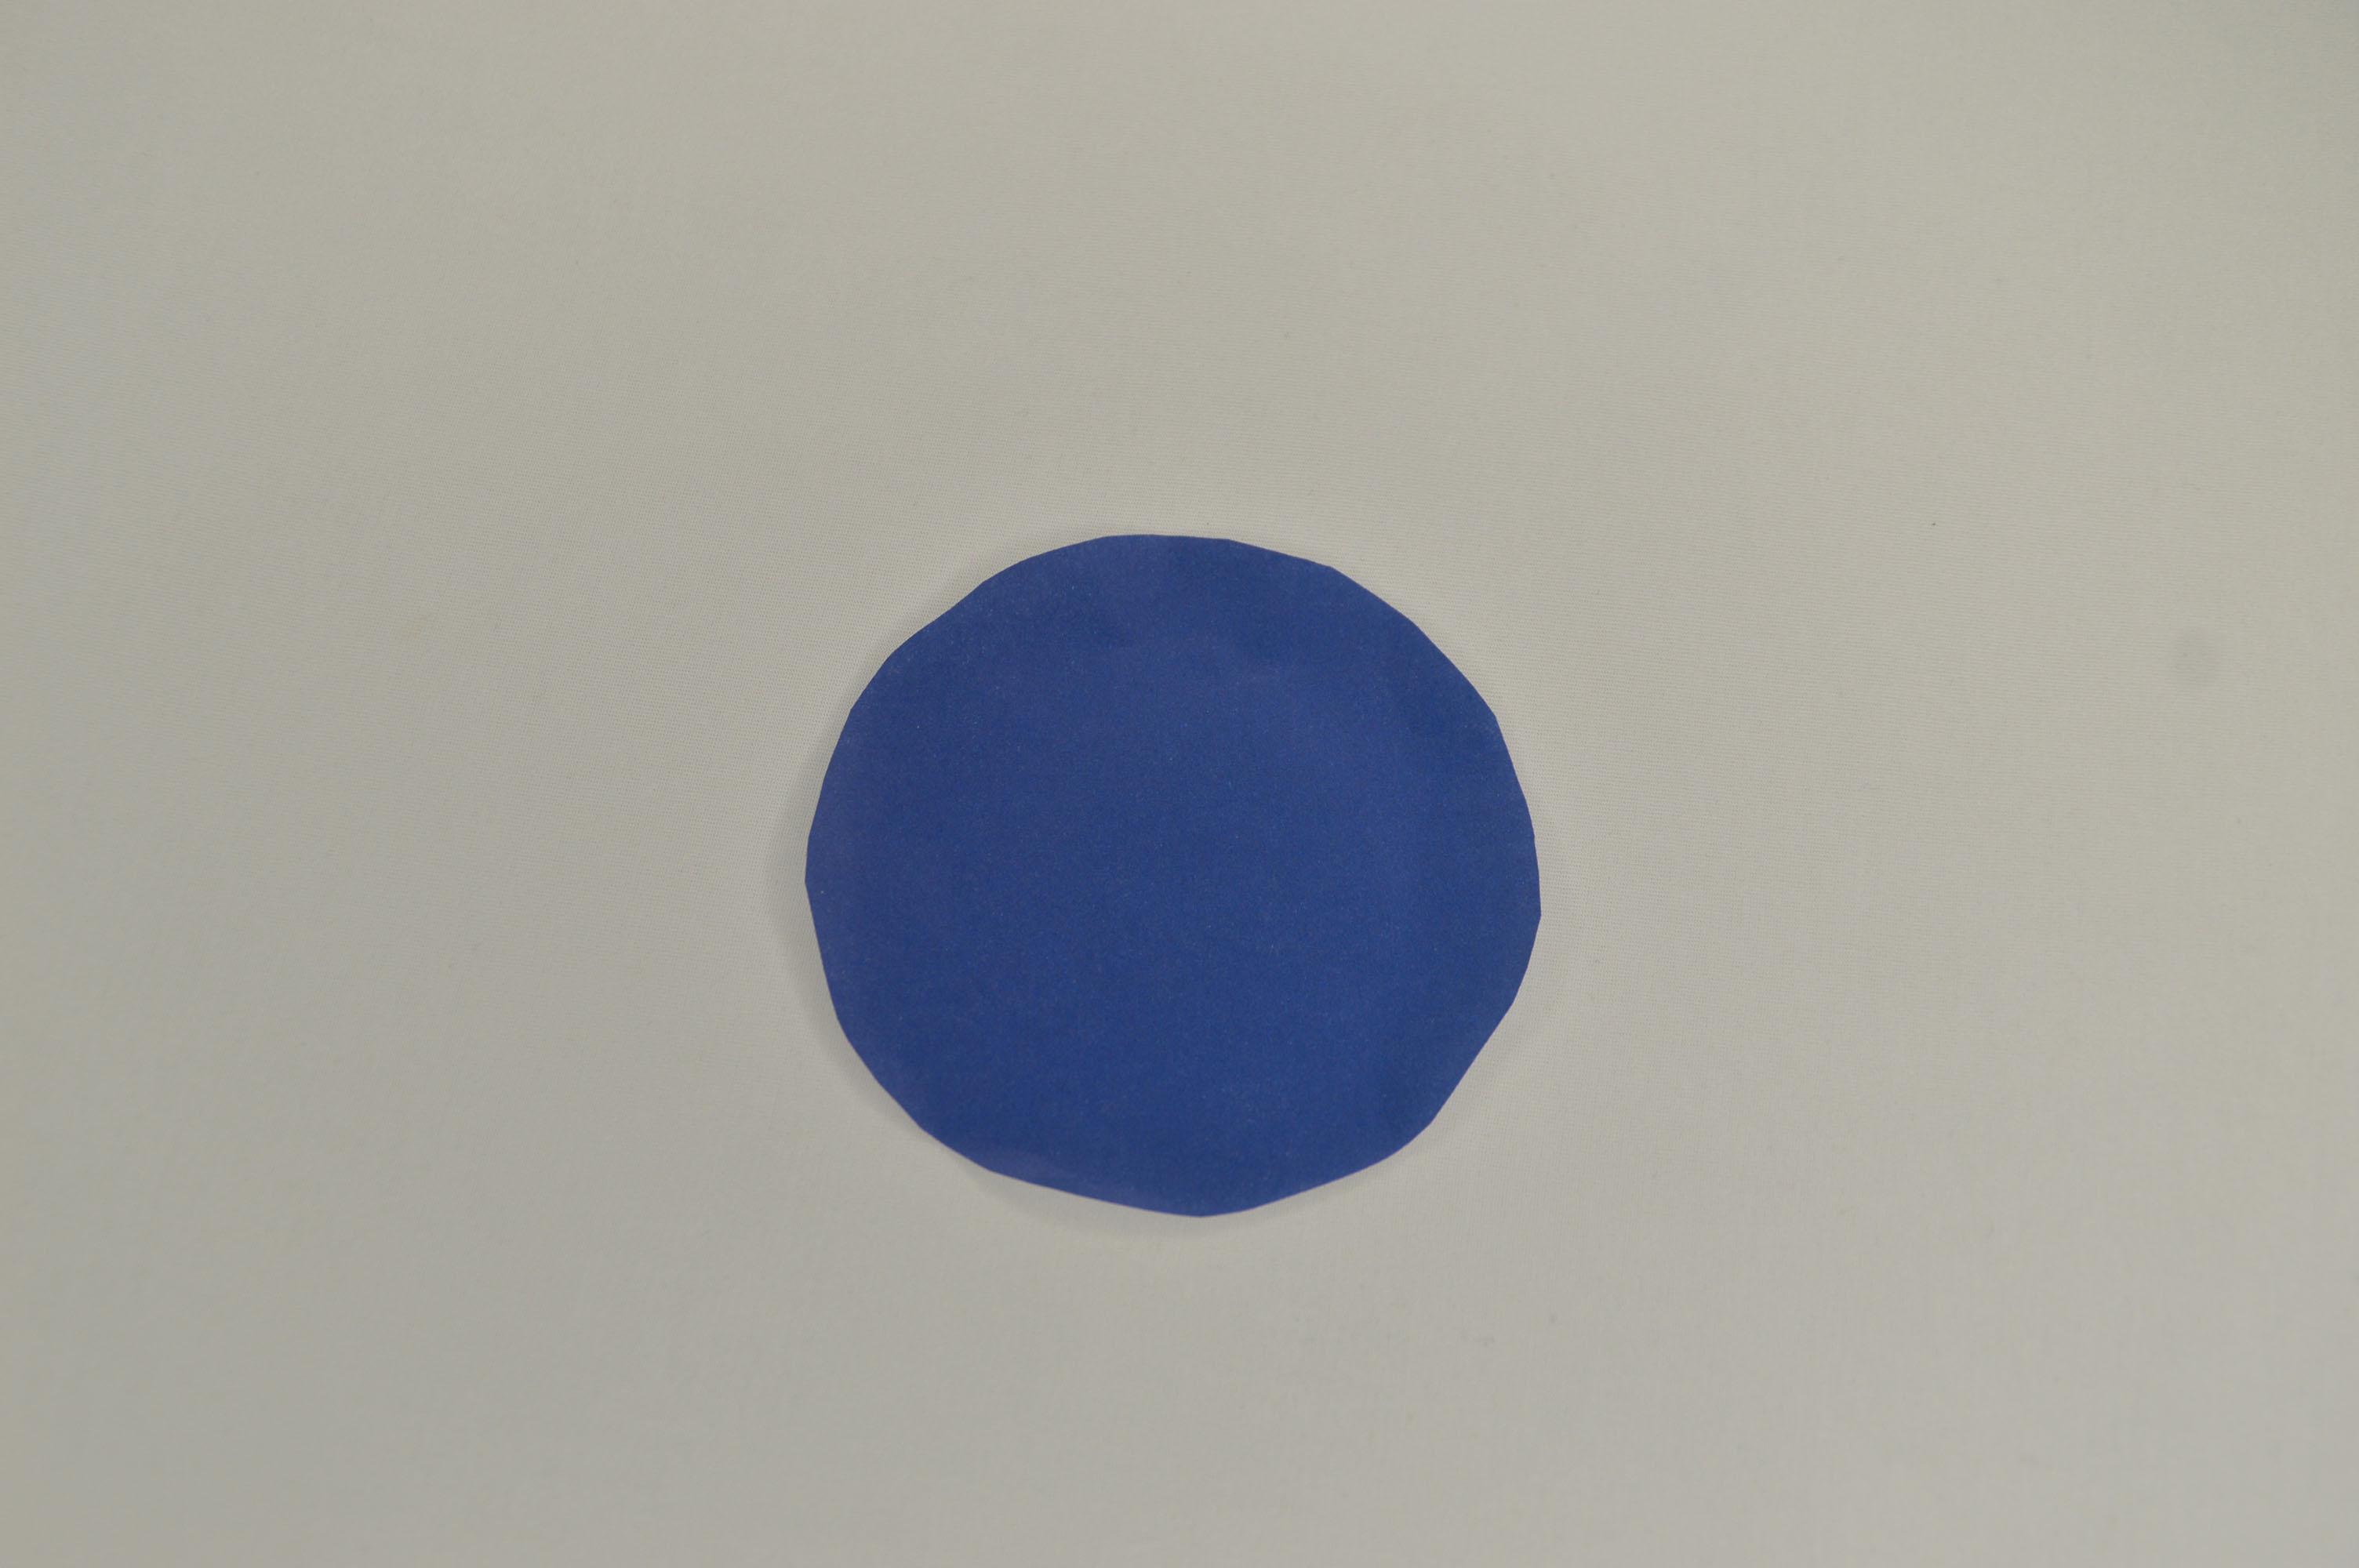
\includegraphics[width=.20\linewidth]{images/train03.jpg}
		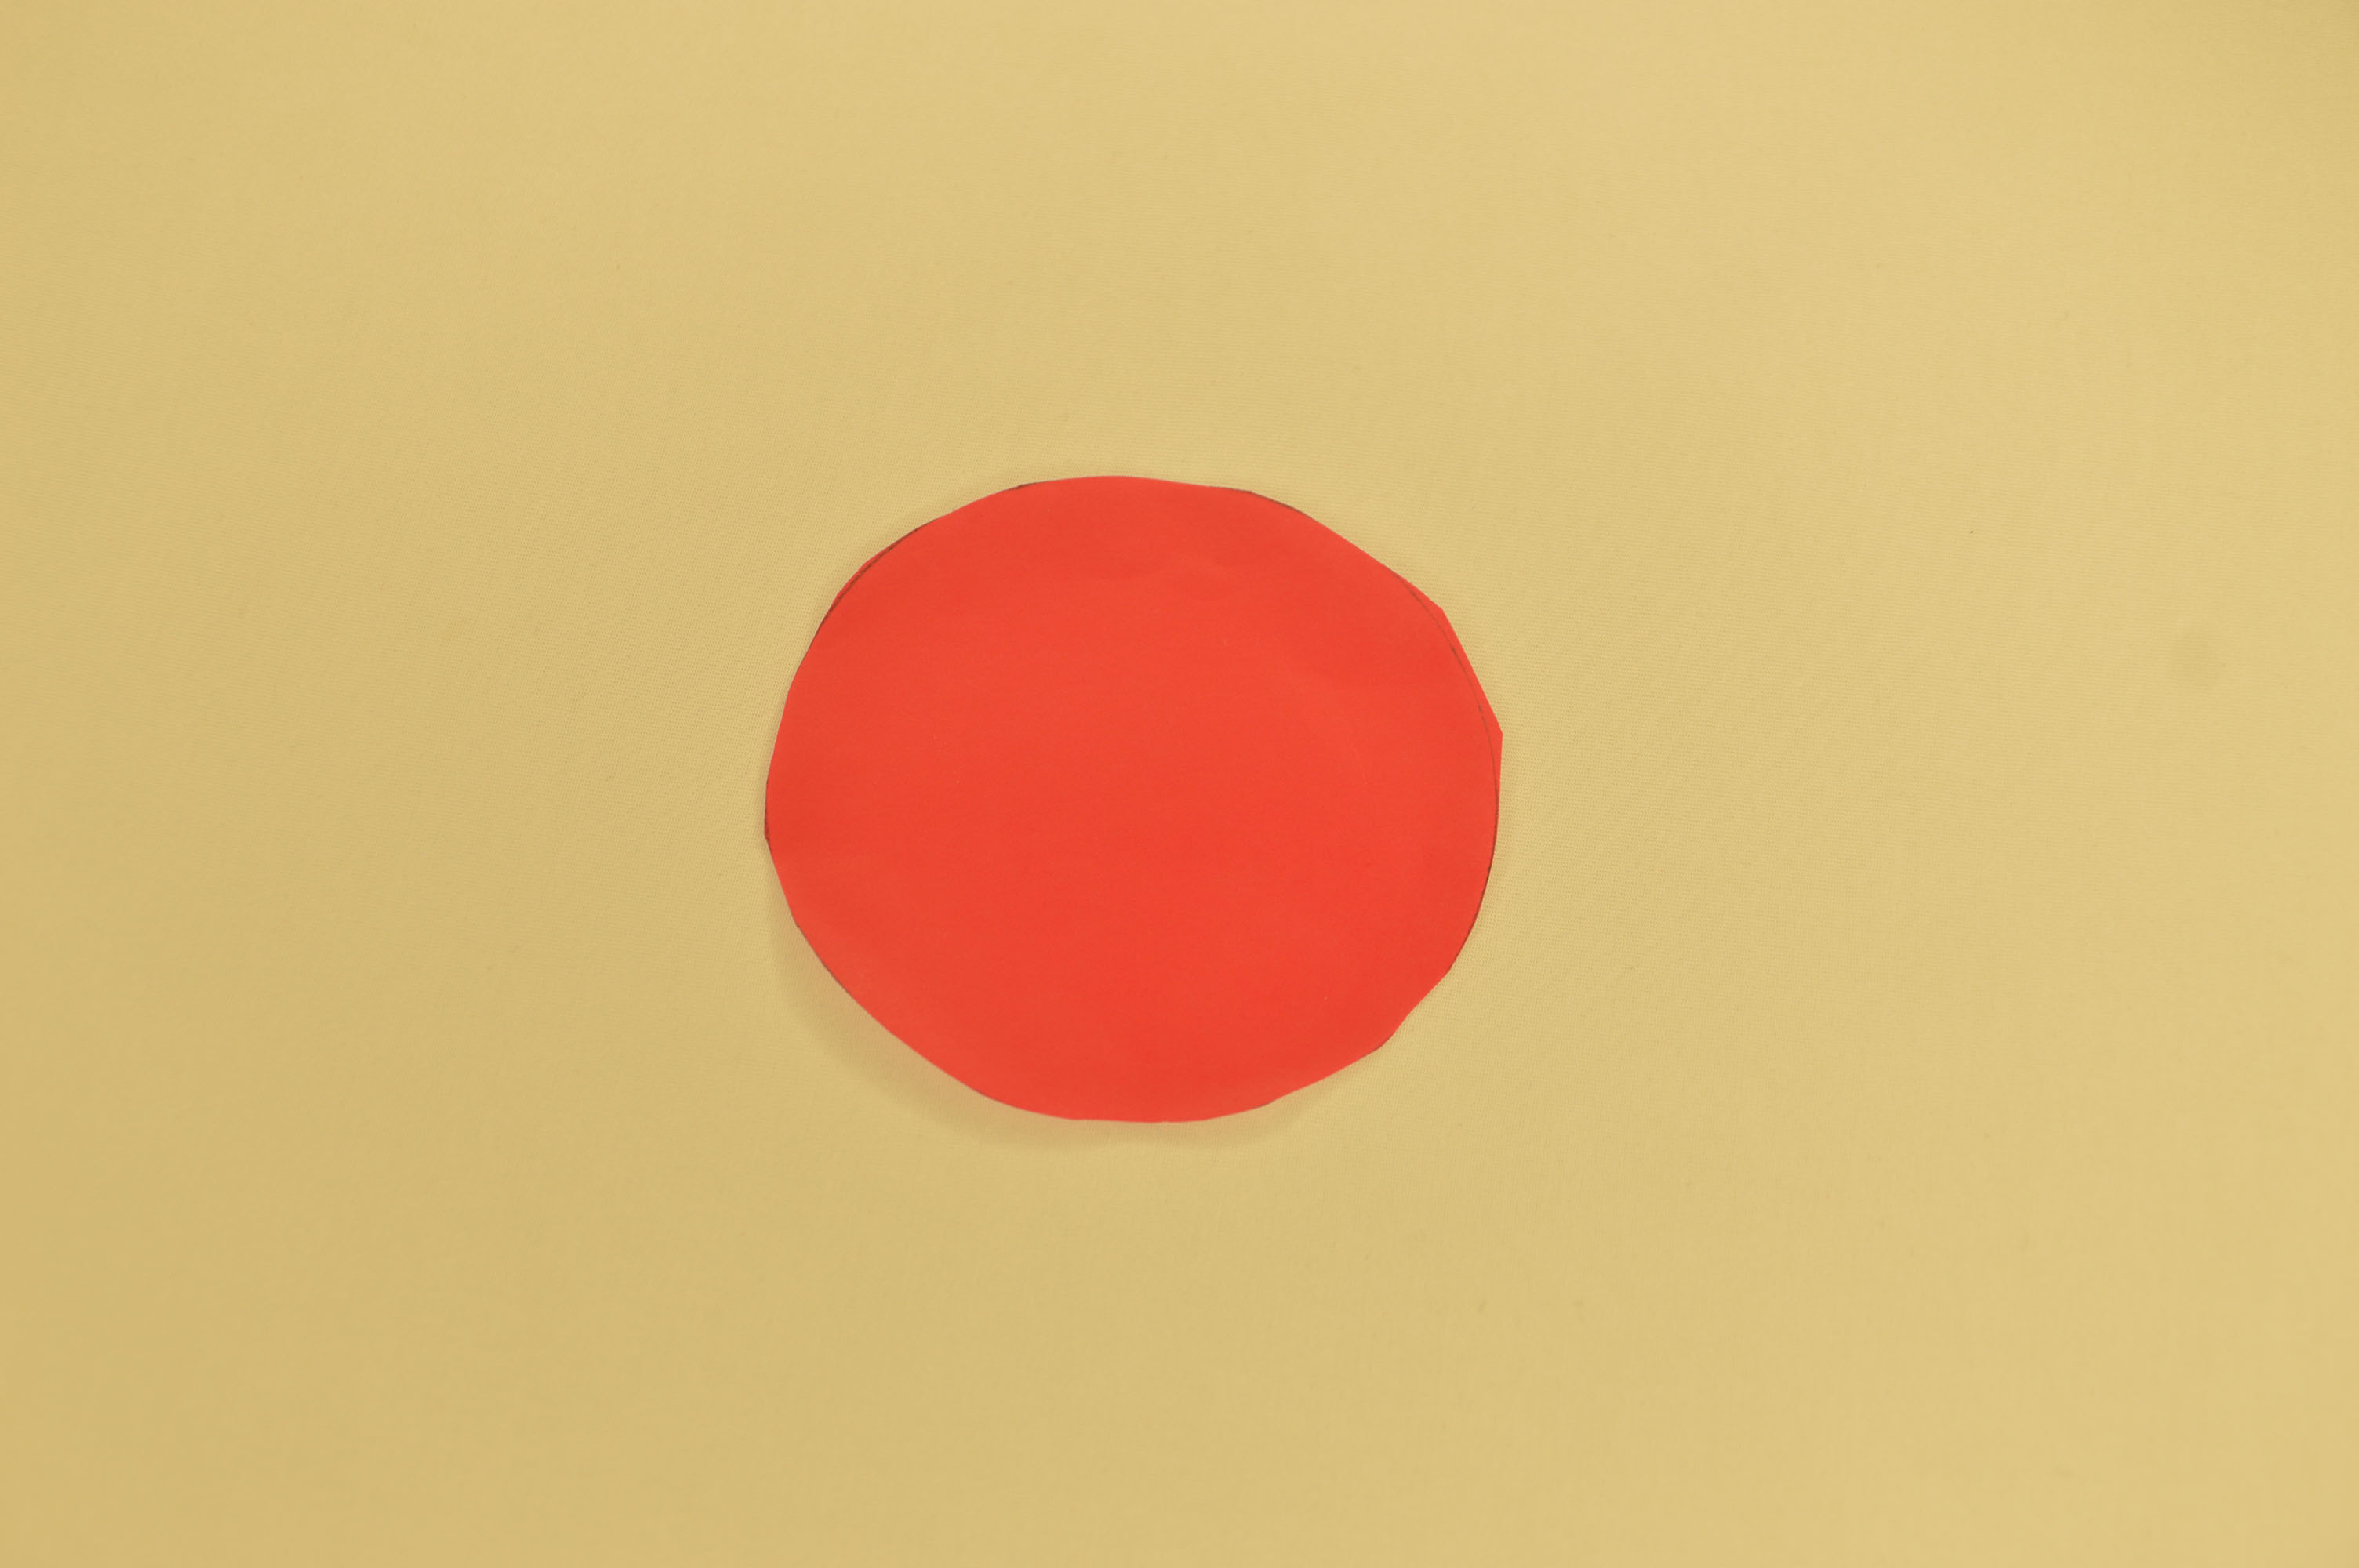
\includegraphics[width=.20\linewidth]{images/train04.jpg} \\
		\vspace{3pt}
		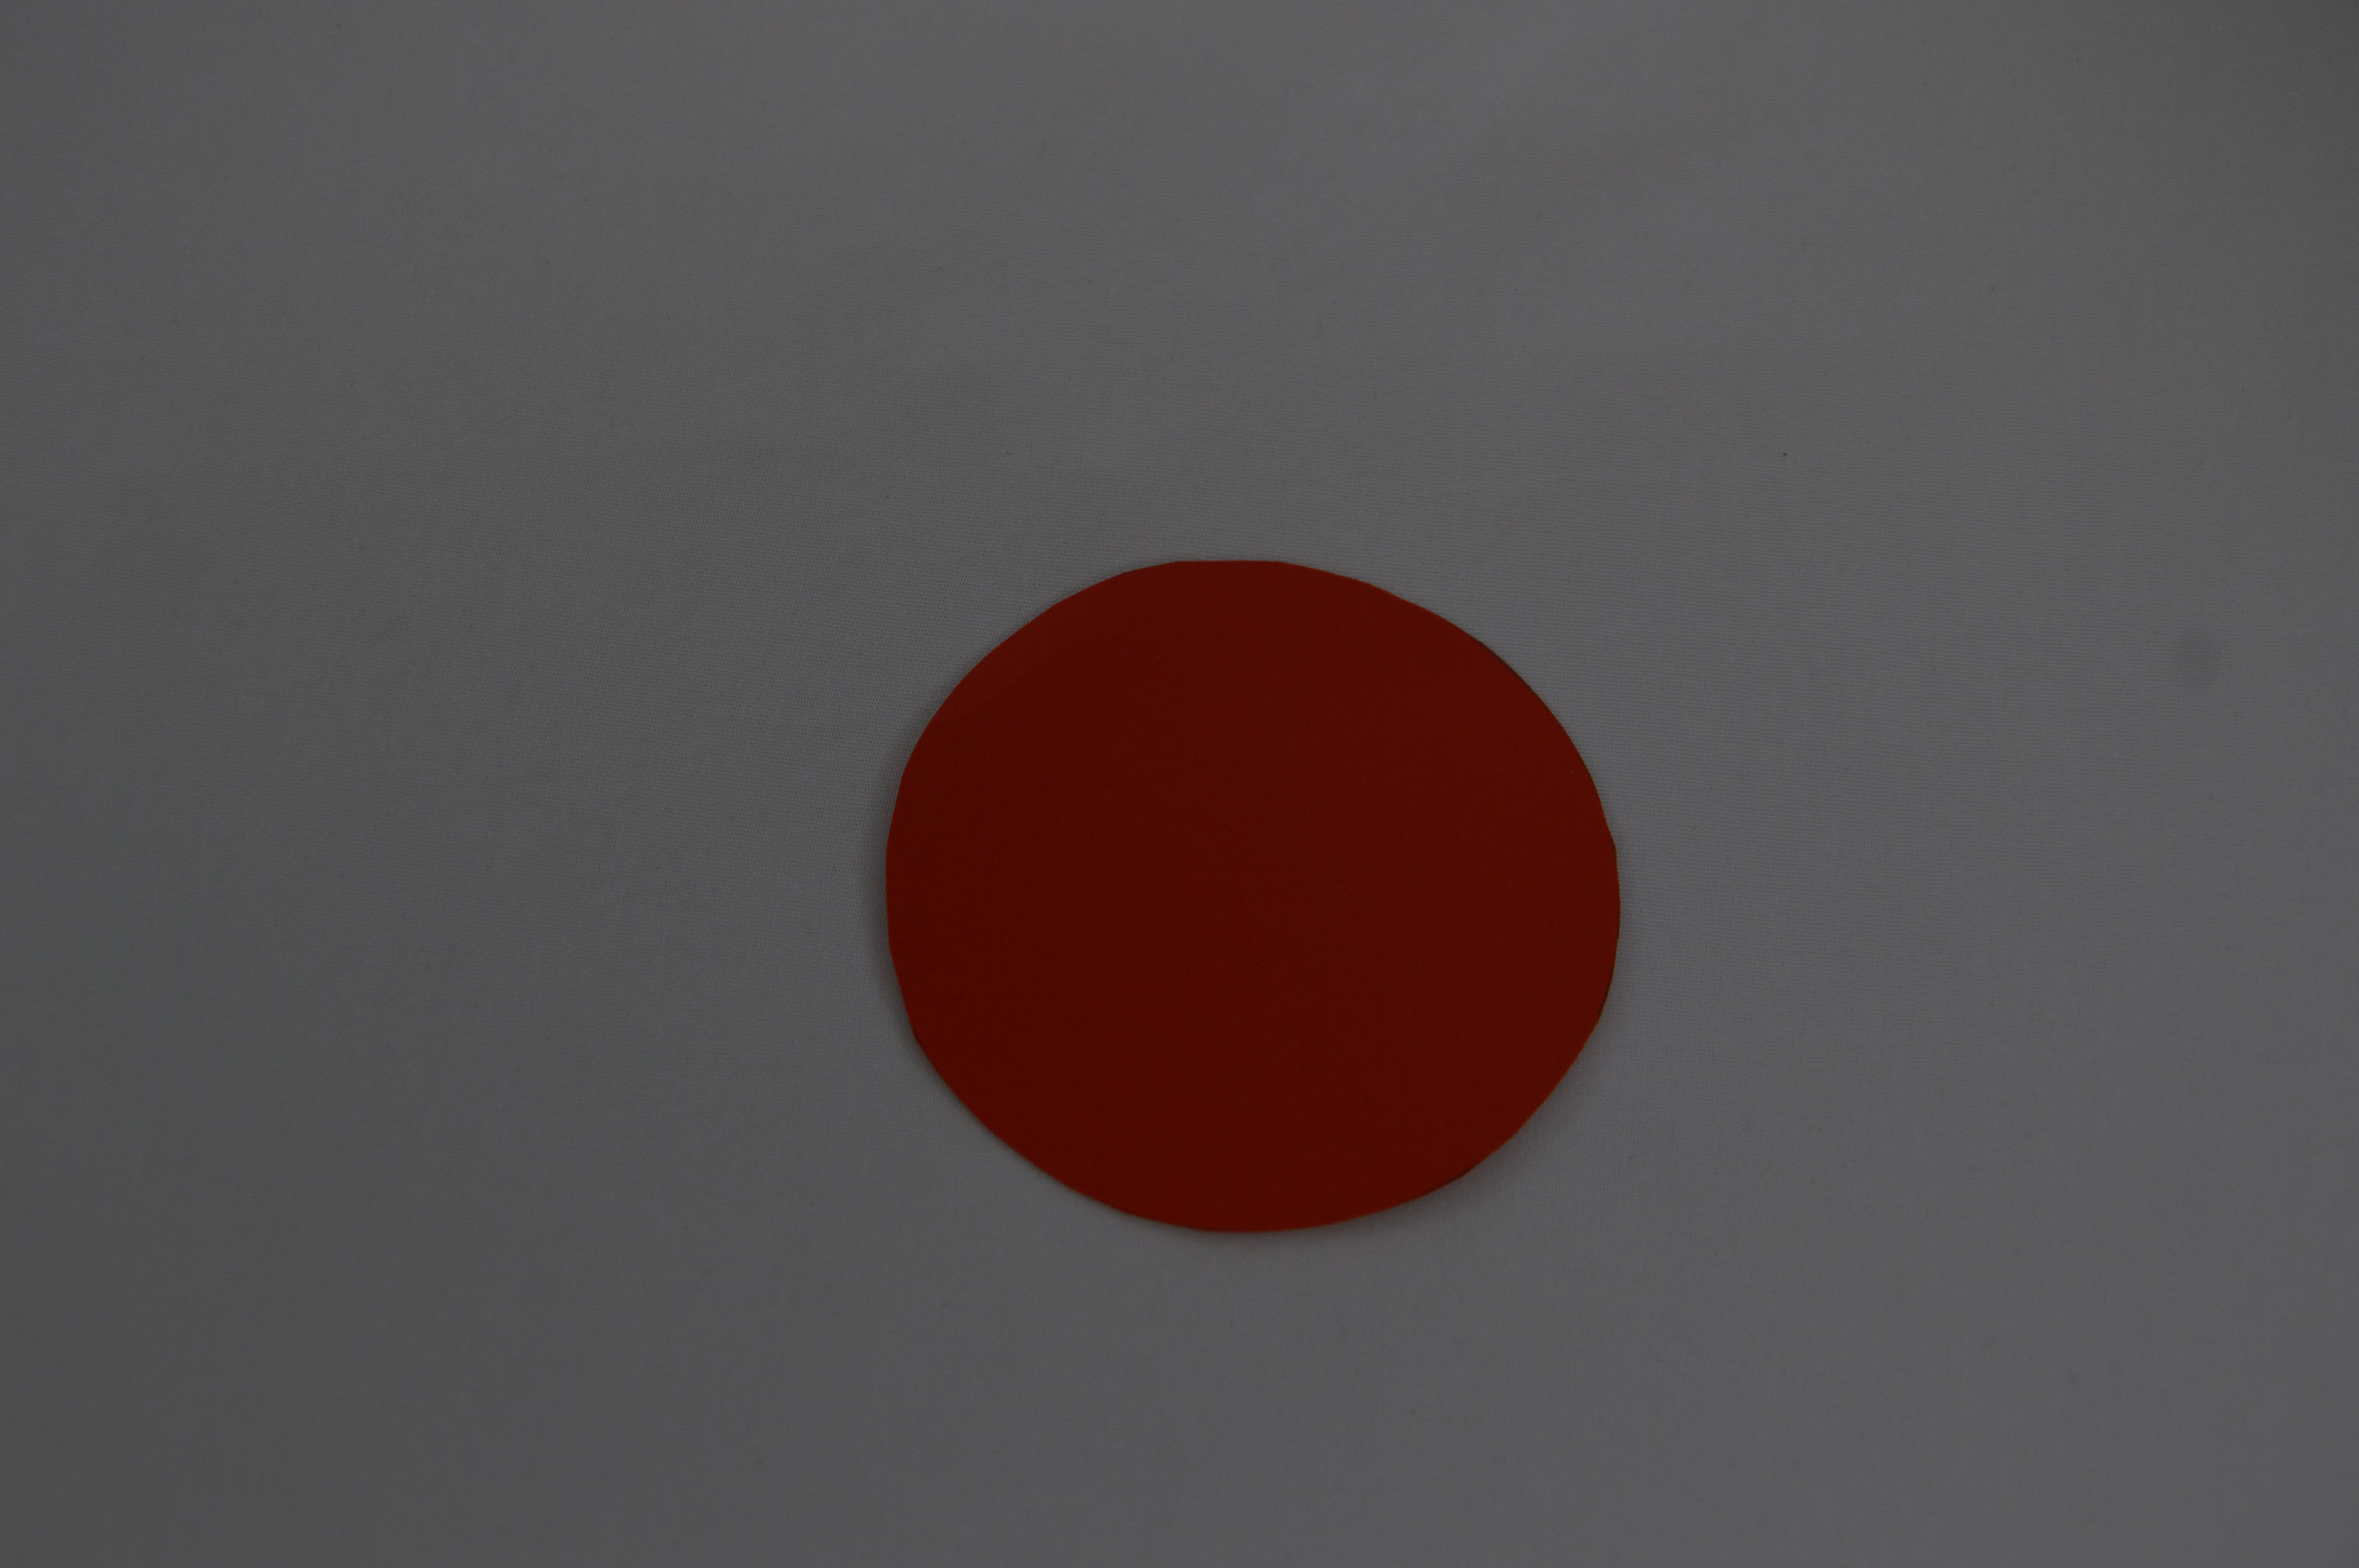
\includegraphics[width=.20\linewidth]{images/train05.jpg}
		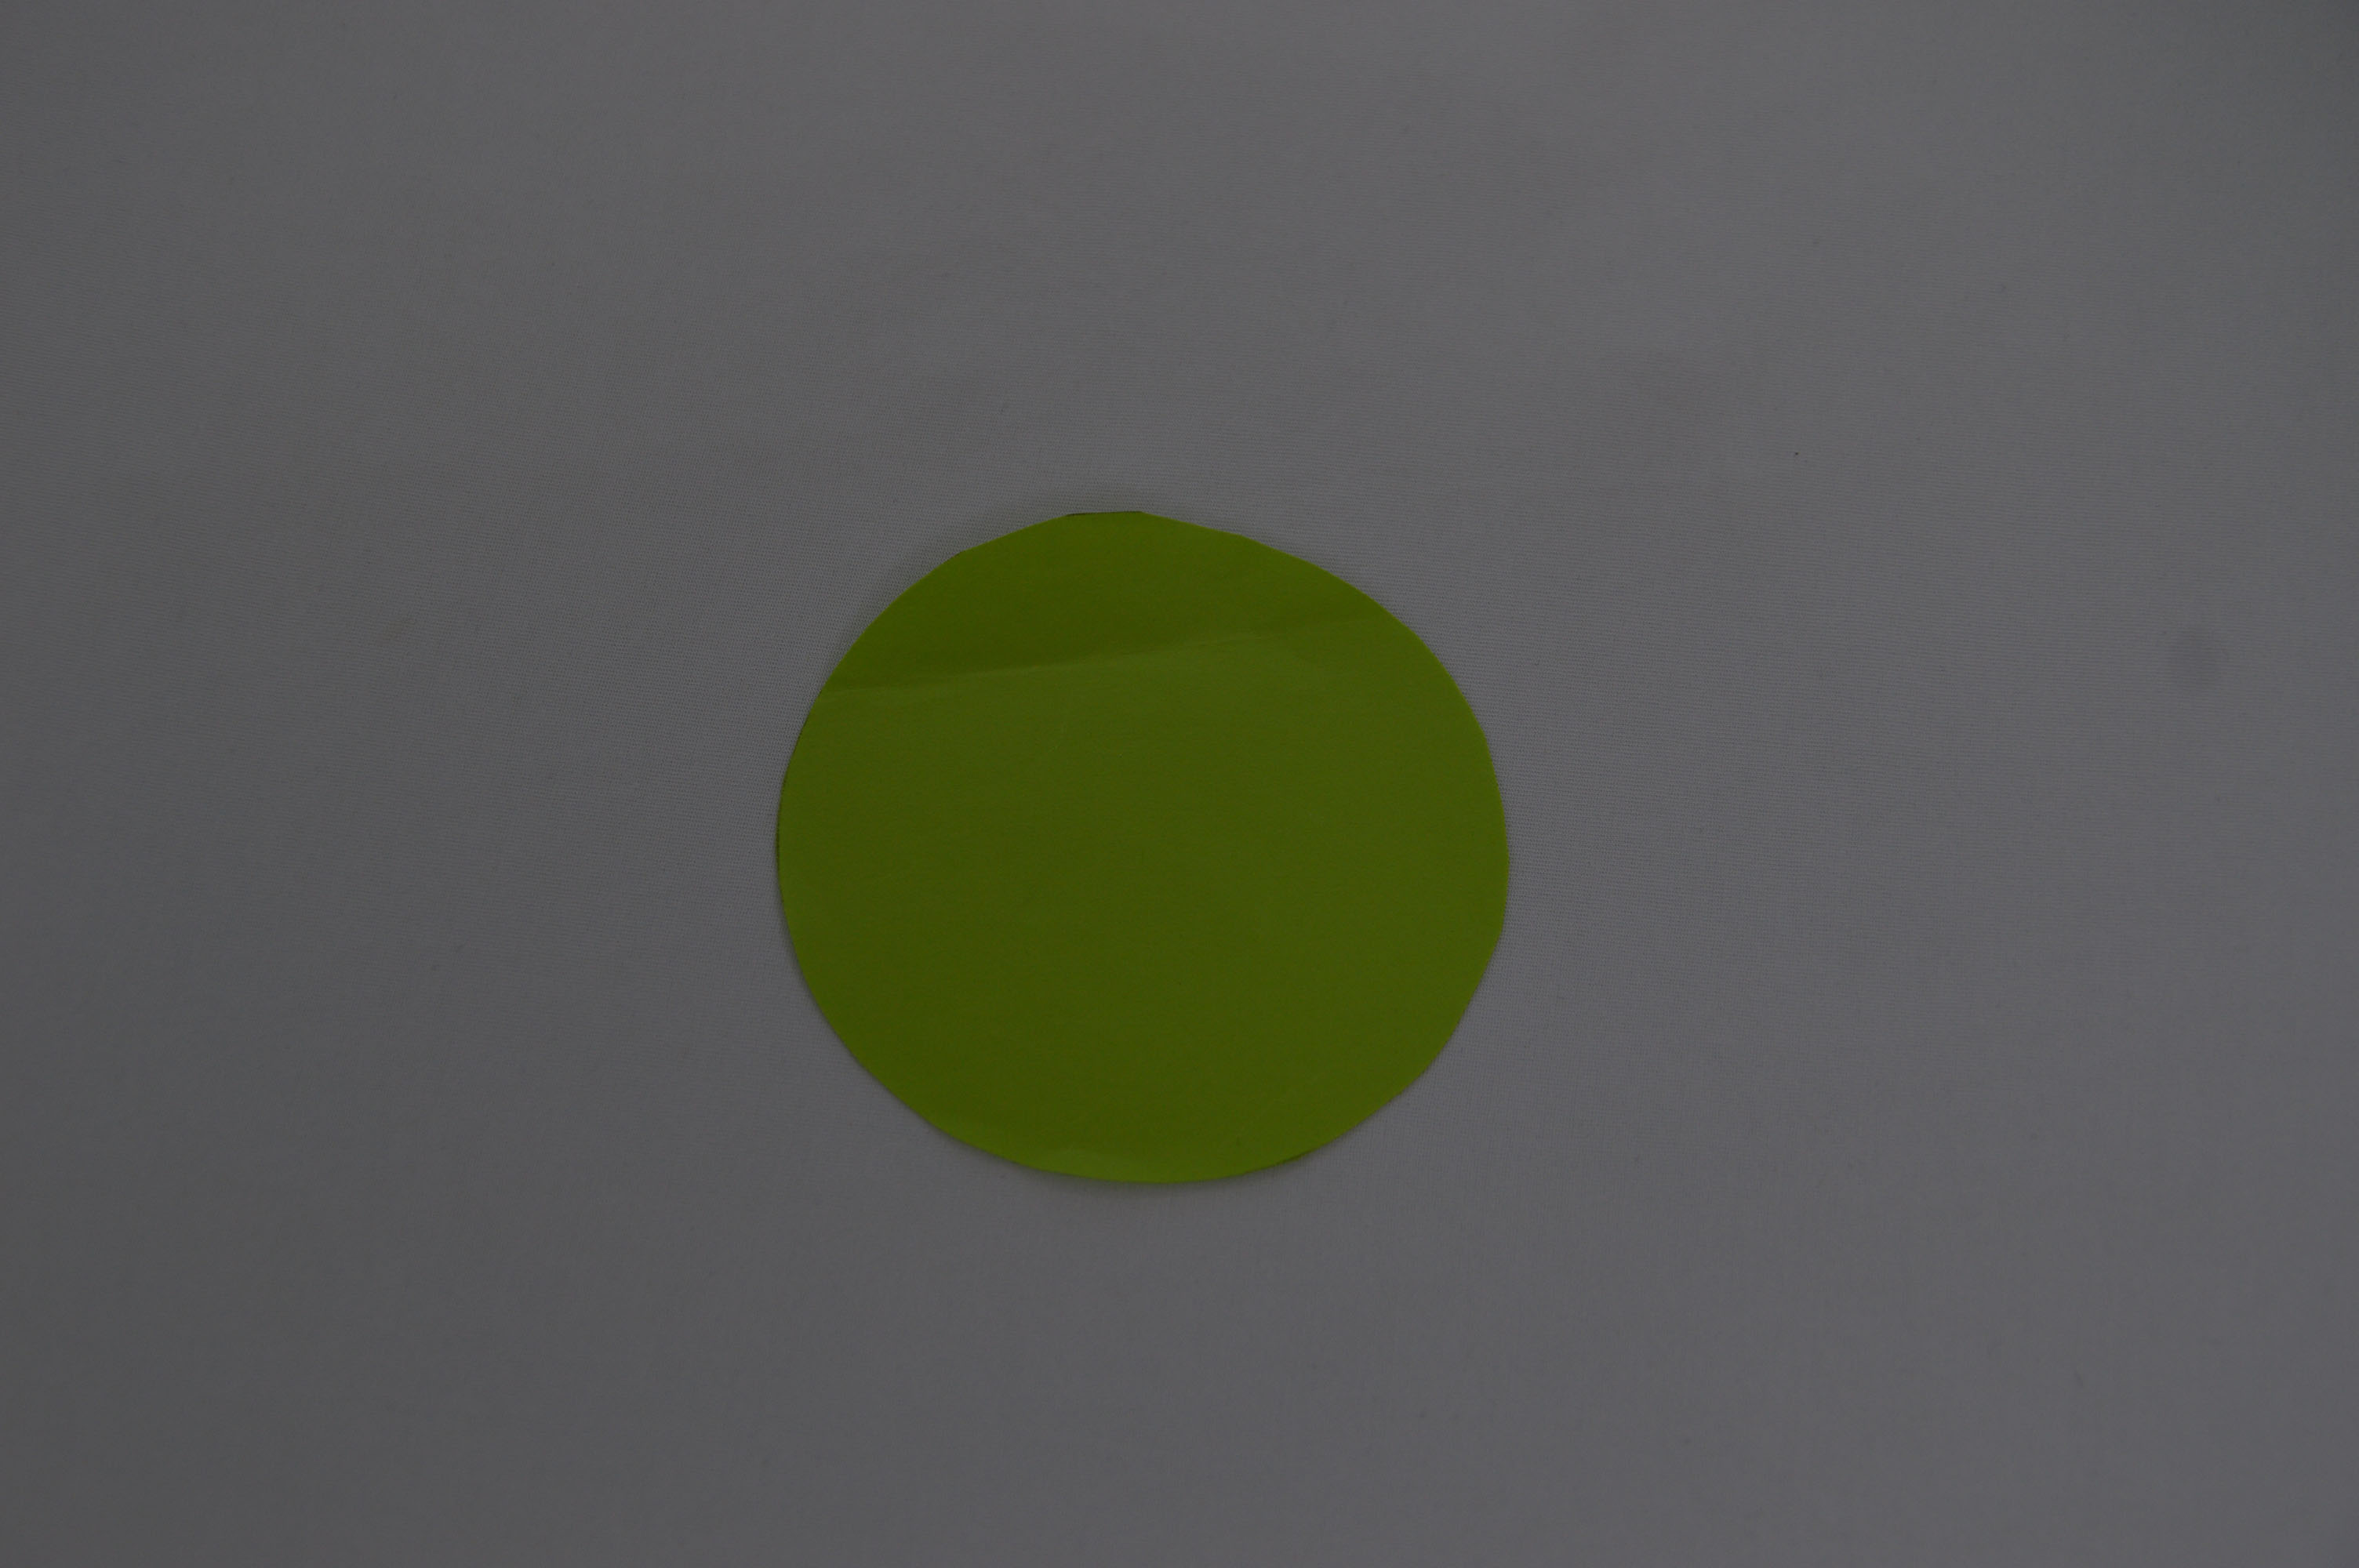
\includegraphics[width=.20\linewidth]{images/train06.jpg}
		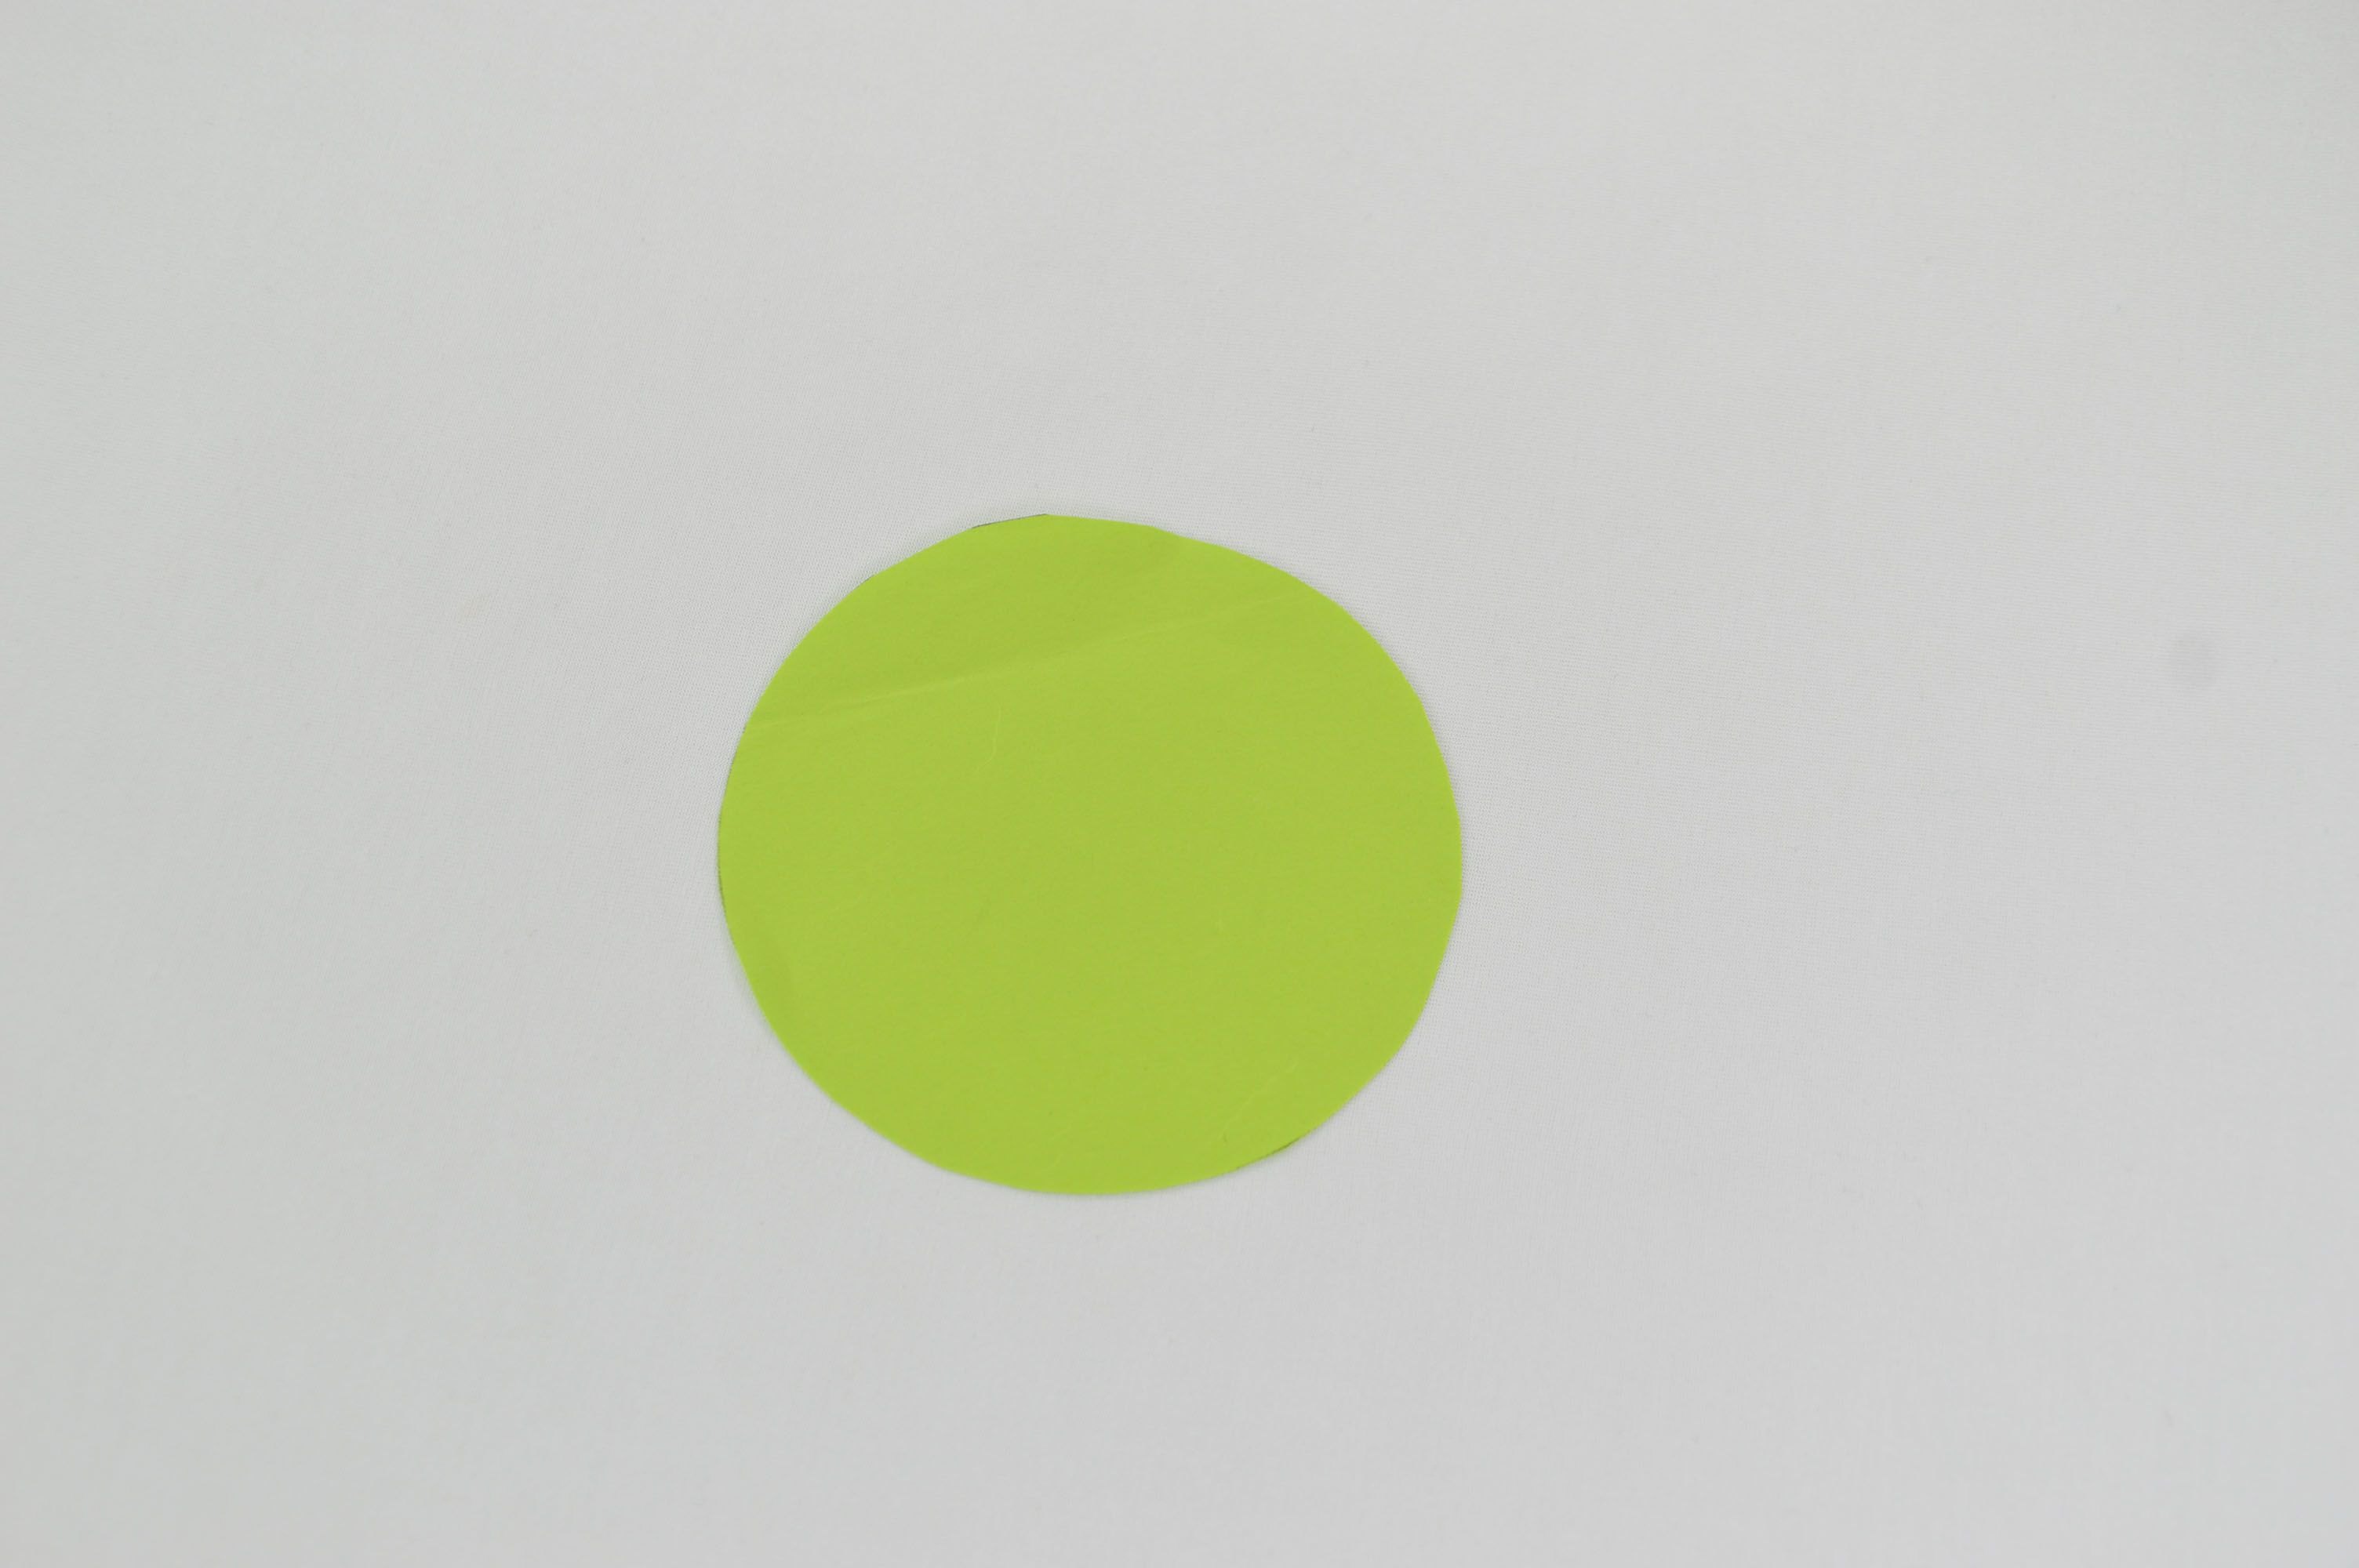
\includegraphics[width=.20\linewidth]{images/train07.jpg}
		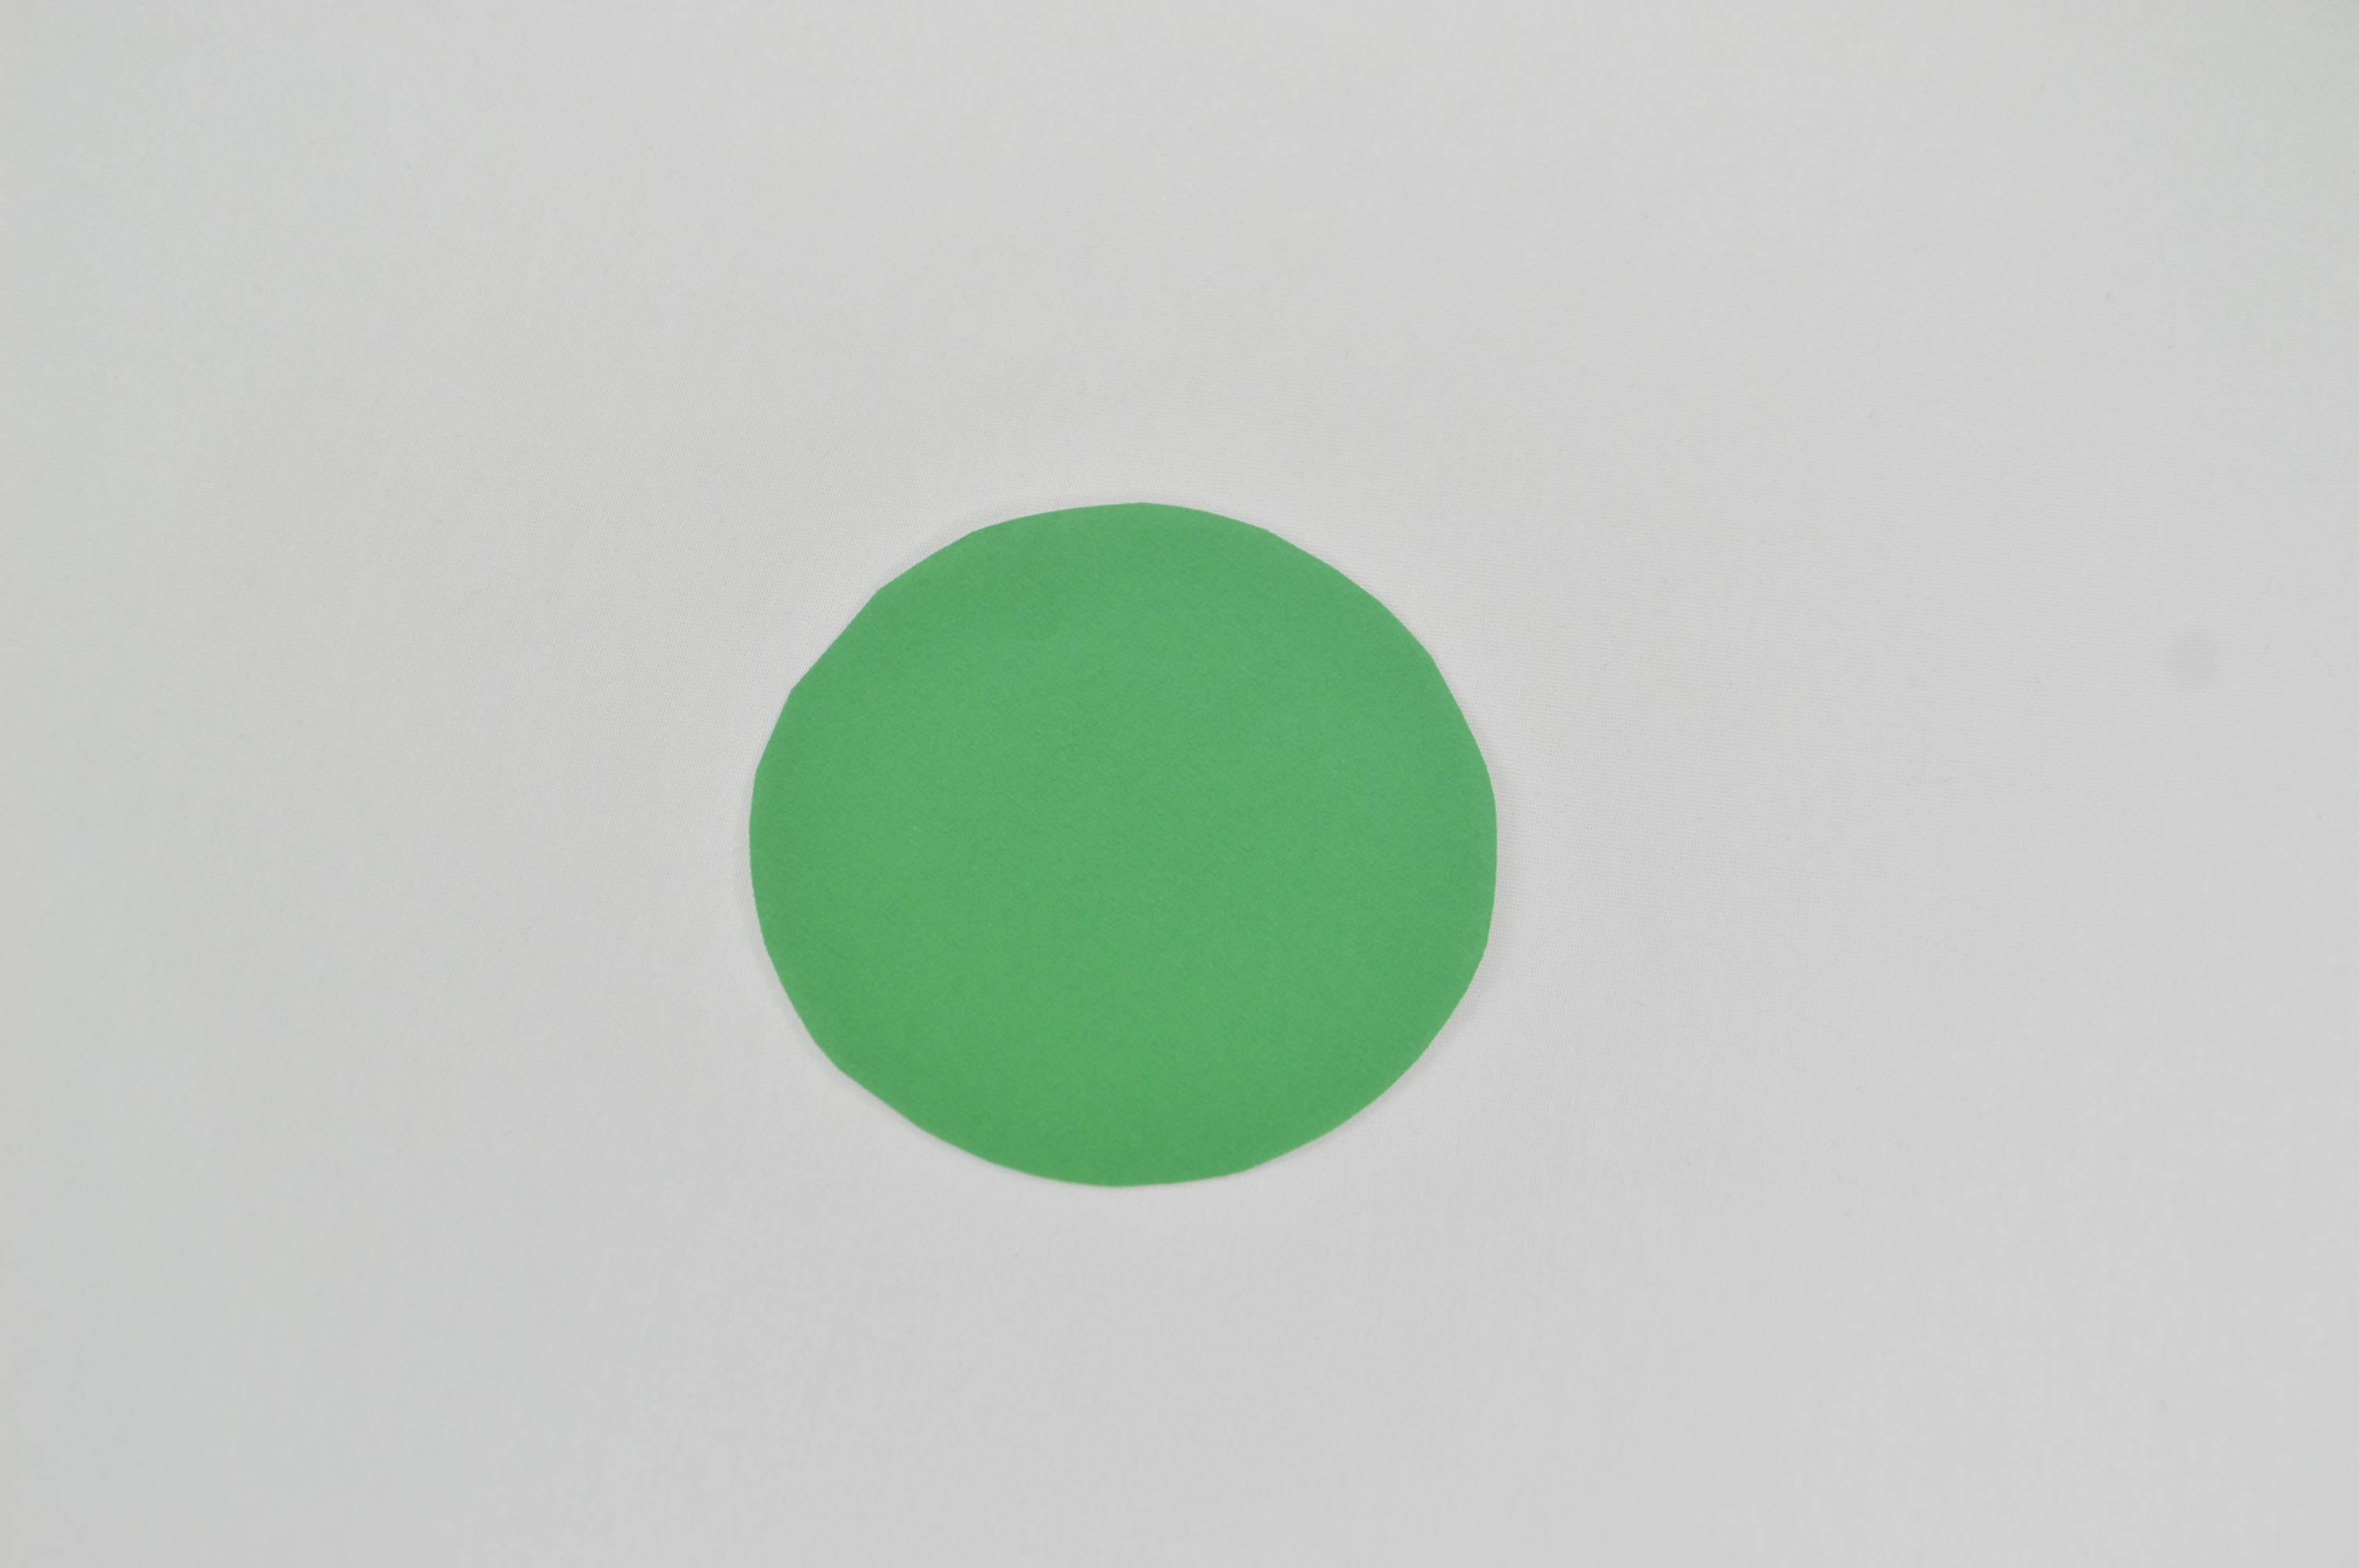
\includegraphics[width=.20\linewidth]{images/train08.jpg}
		\caption{First set of photos}
	\end{figure}

	For the second set of images, we took photos of single coloured cylinders from different sides with a "fixed" light source, the sun. All the cylinders had roughly the same diameter as they were created by wrapping paper around a plastic bottle. We used paper of different shades of each colour and of different textures. \\
	
	Photos were taken when the sun was low, so the light was hitting the cylinder more horizontally than vertically. Pictures were taken from 3 viewing points - towards the sunlight, against the sunlight and perpendicular to the sunlight direction. This ensured somewhat gradient distribution of the cololor in the images. This is important, because cylinders that the robot will encounter will also have gradient distribution of the colour.\\
	
	We obtained around 130 photos of this kind. A subset of the images is included below.
	
	\begin{figure}[H]
		\centering
		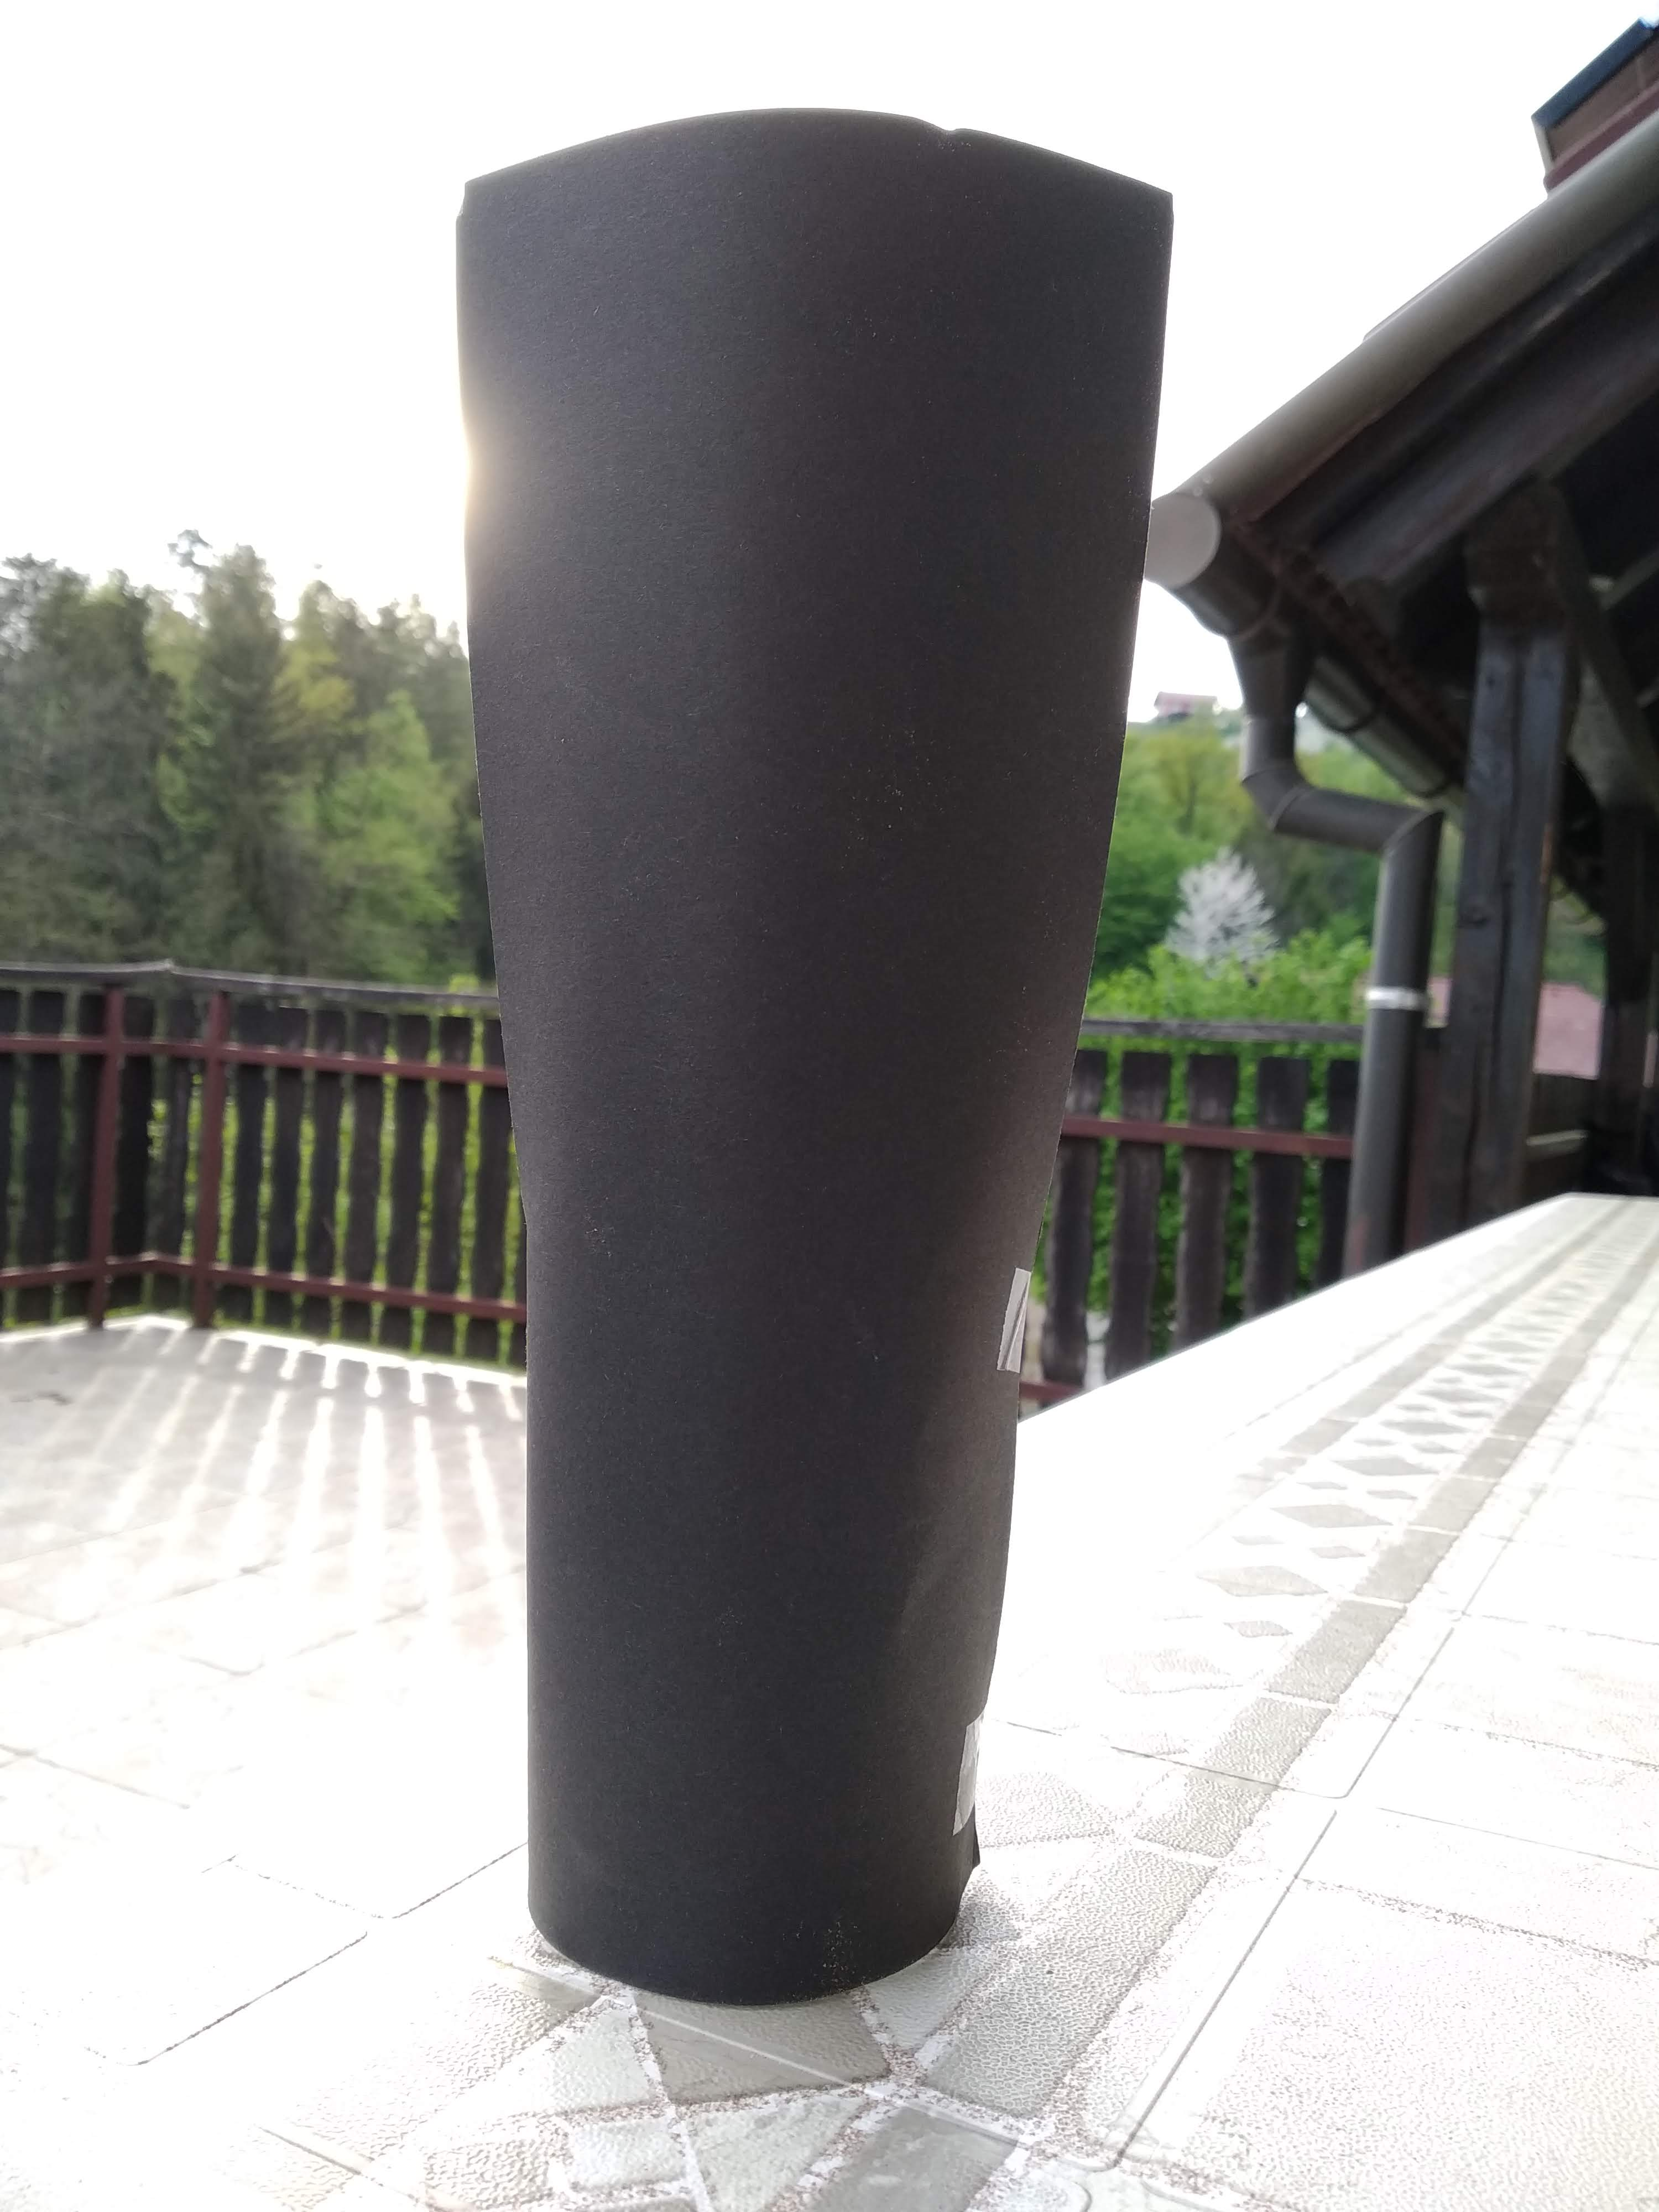
\includegraphics[width=.13\linewidth]{images/test01.jpg}
		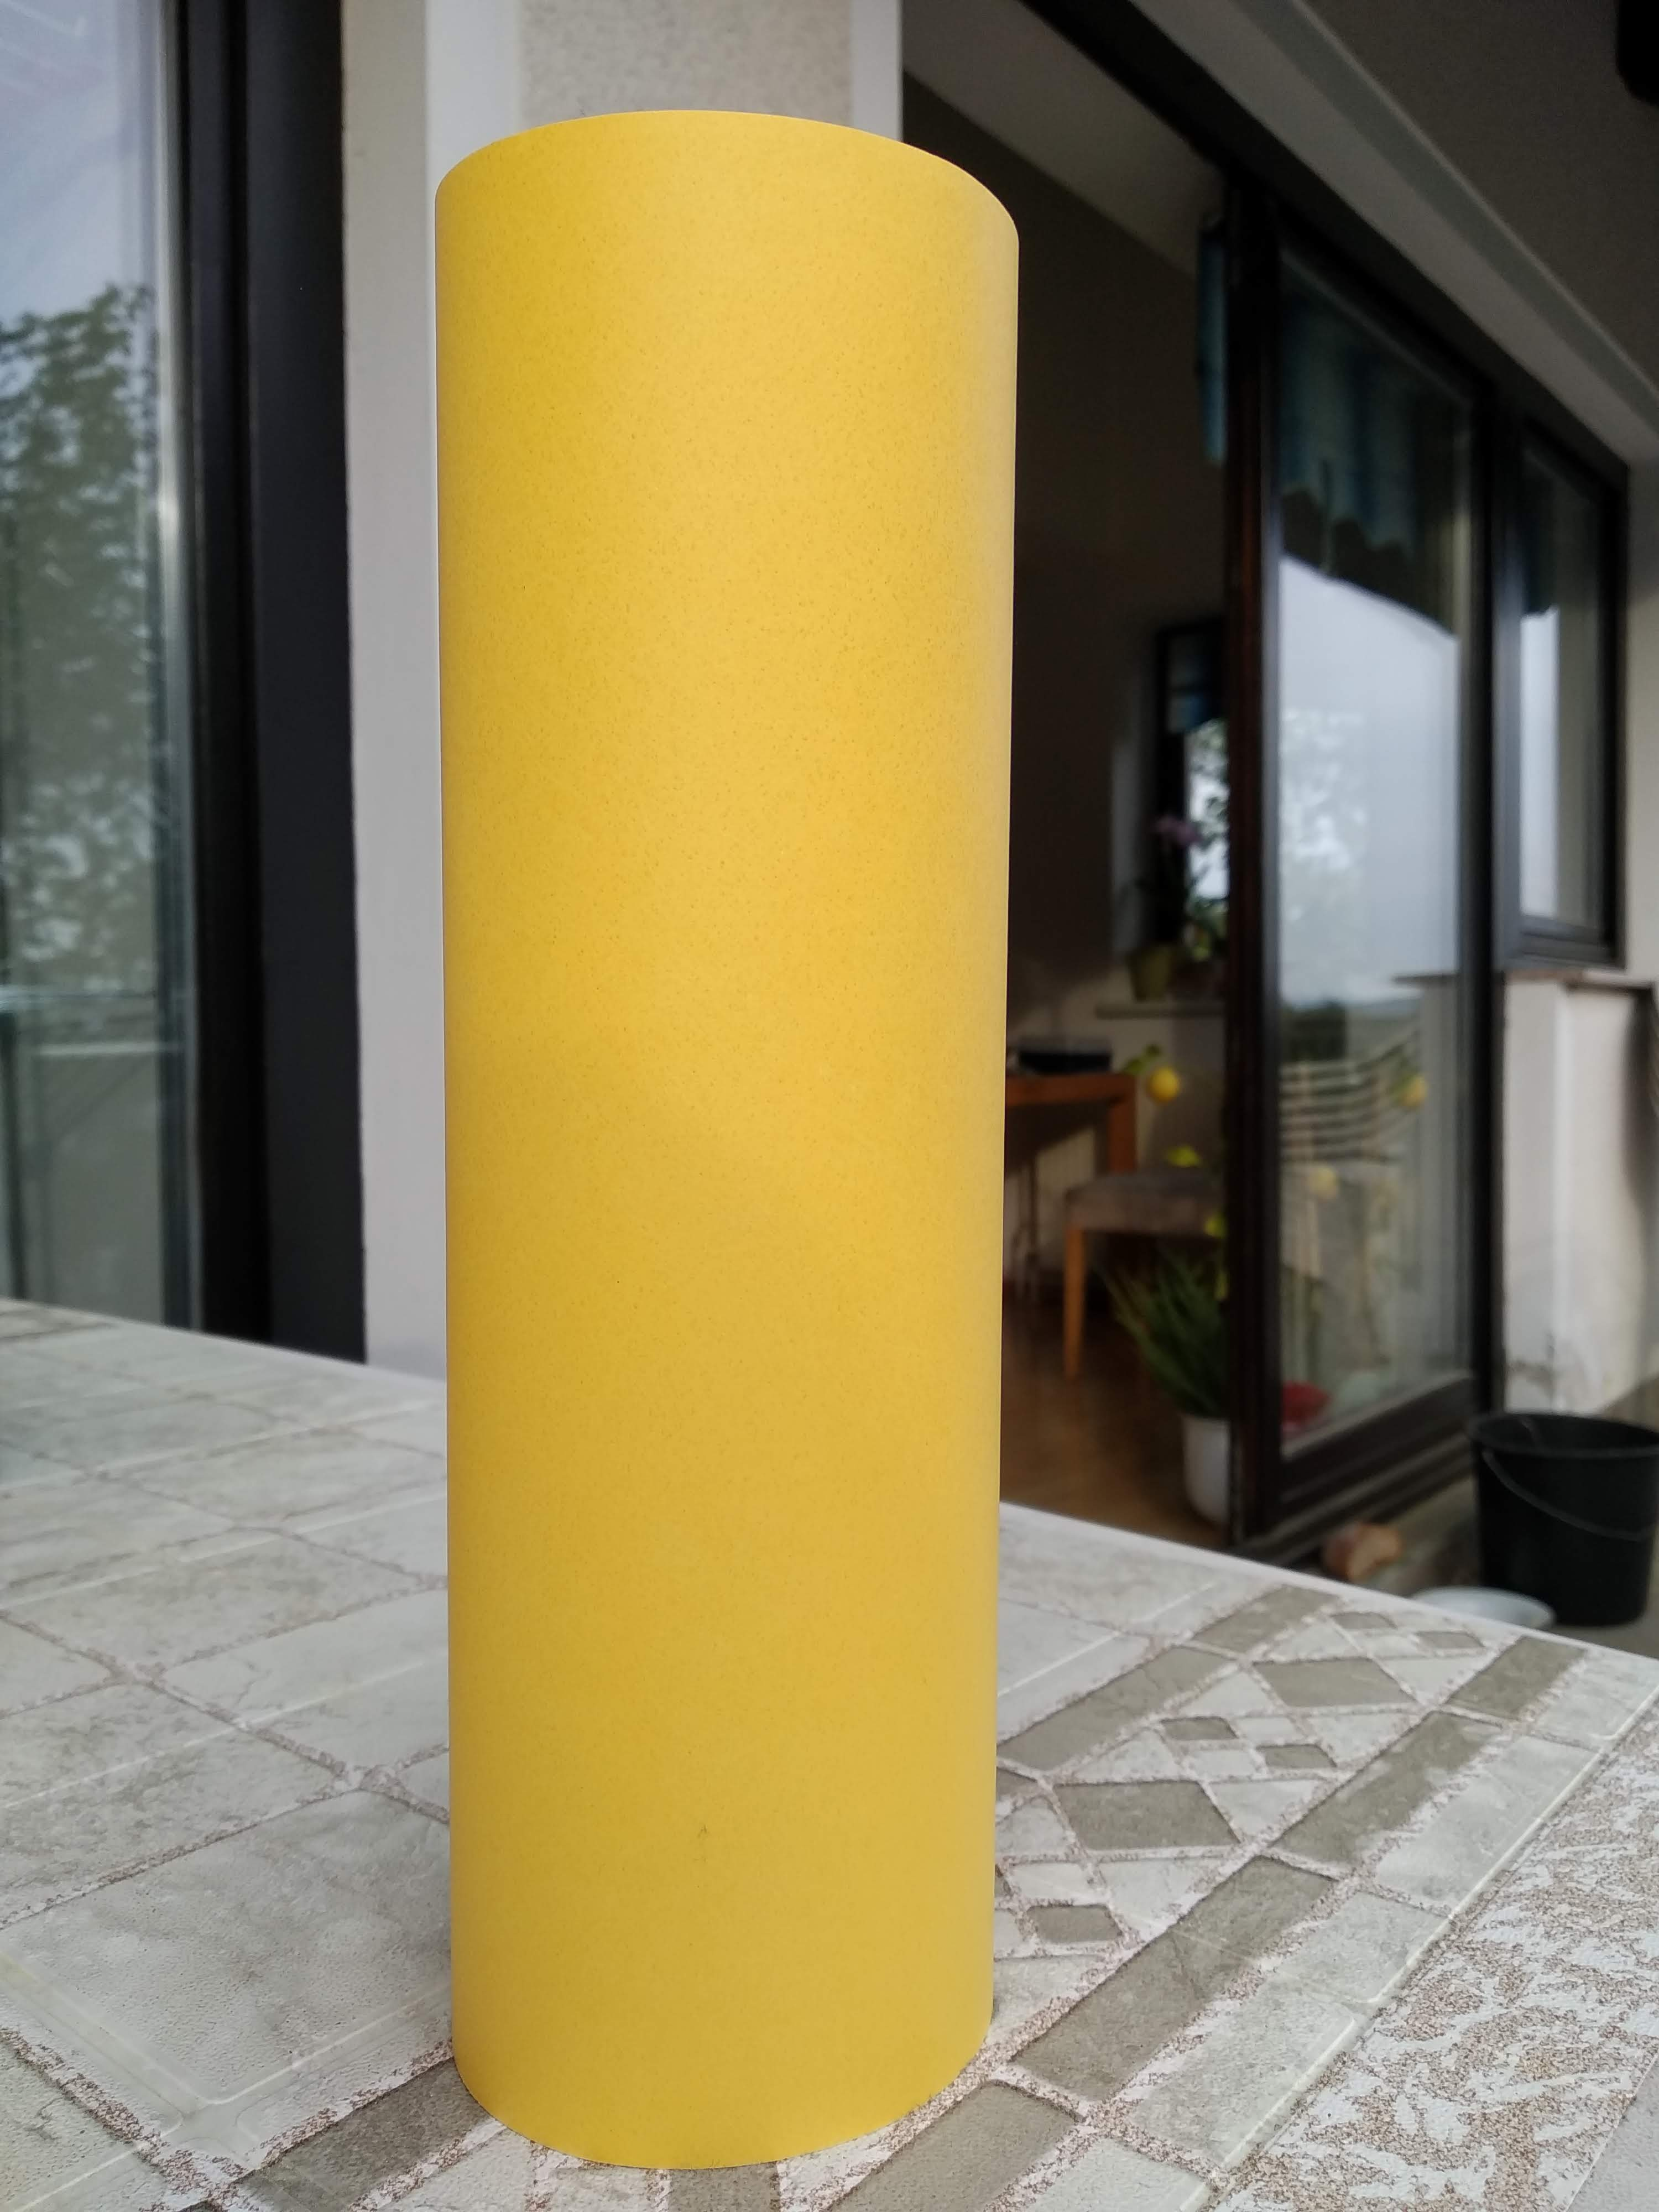
\includegraphics[width=.13\linewidth]{images/test02.jpg}
		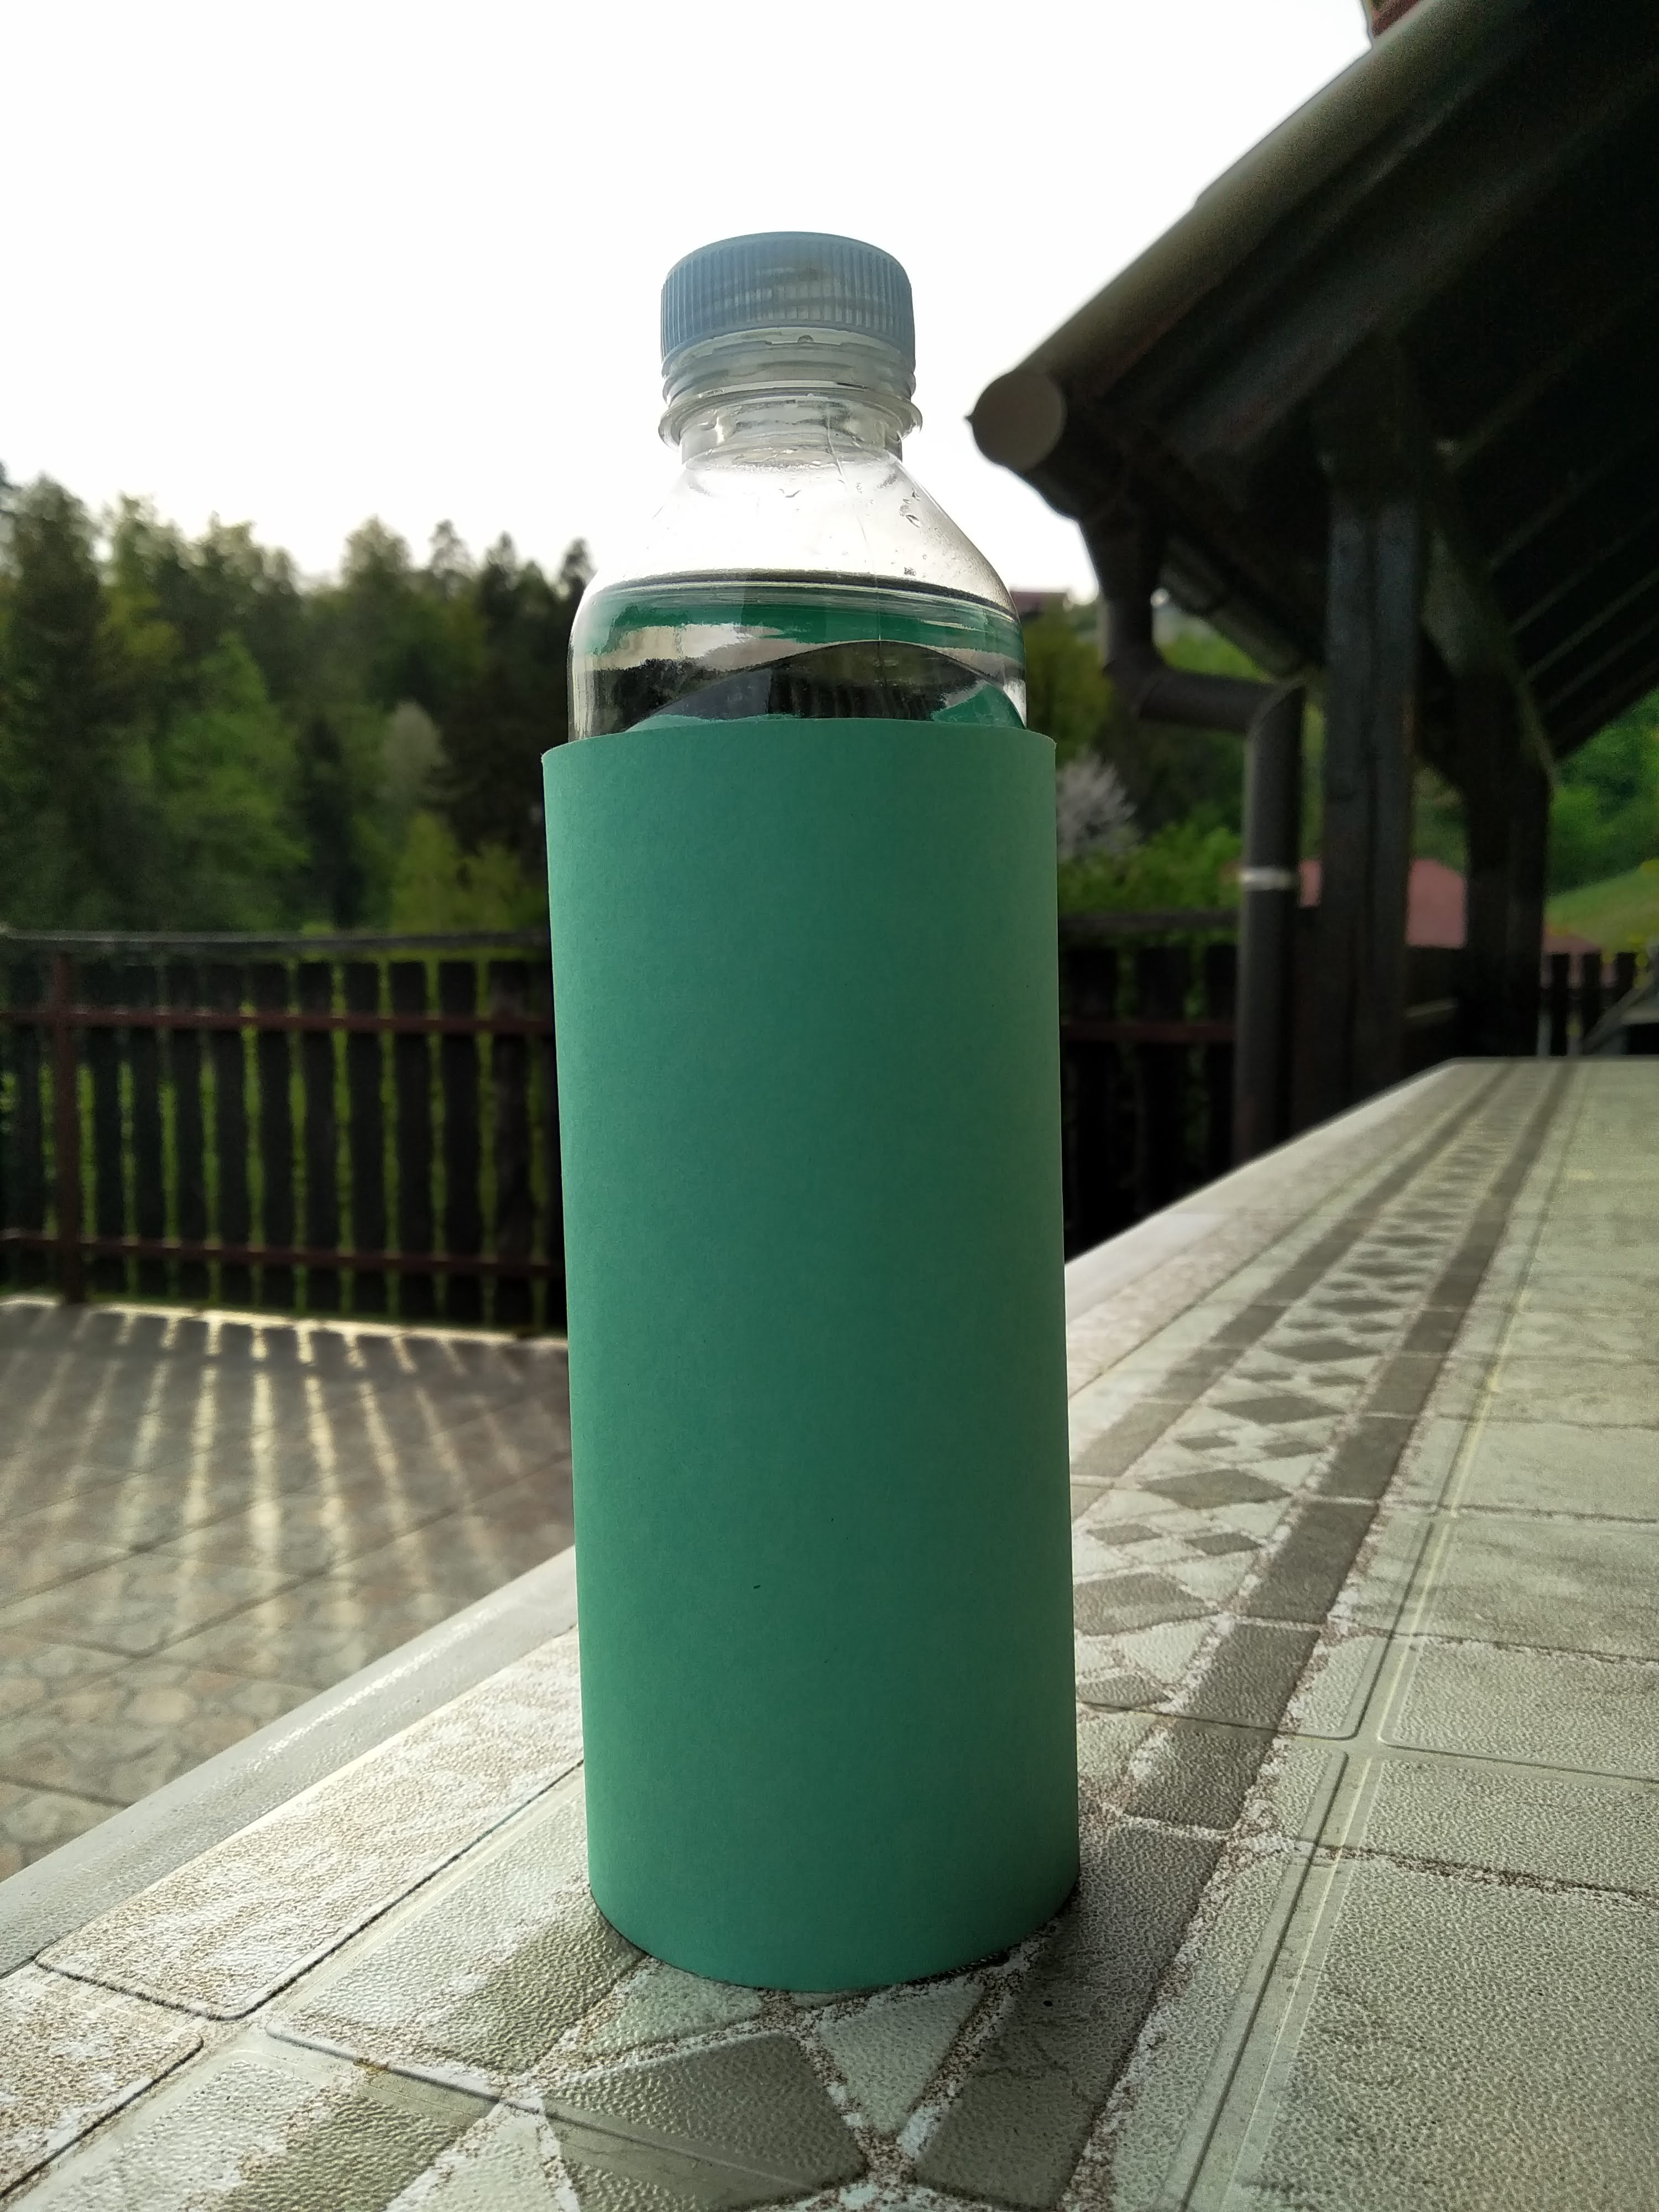
\includegraphics[width=.13\linewidth]{images/test03.jpg}
		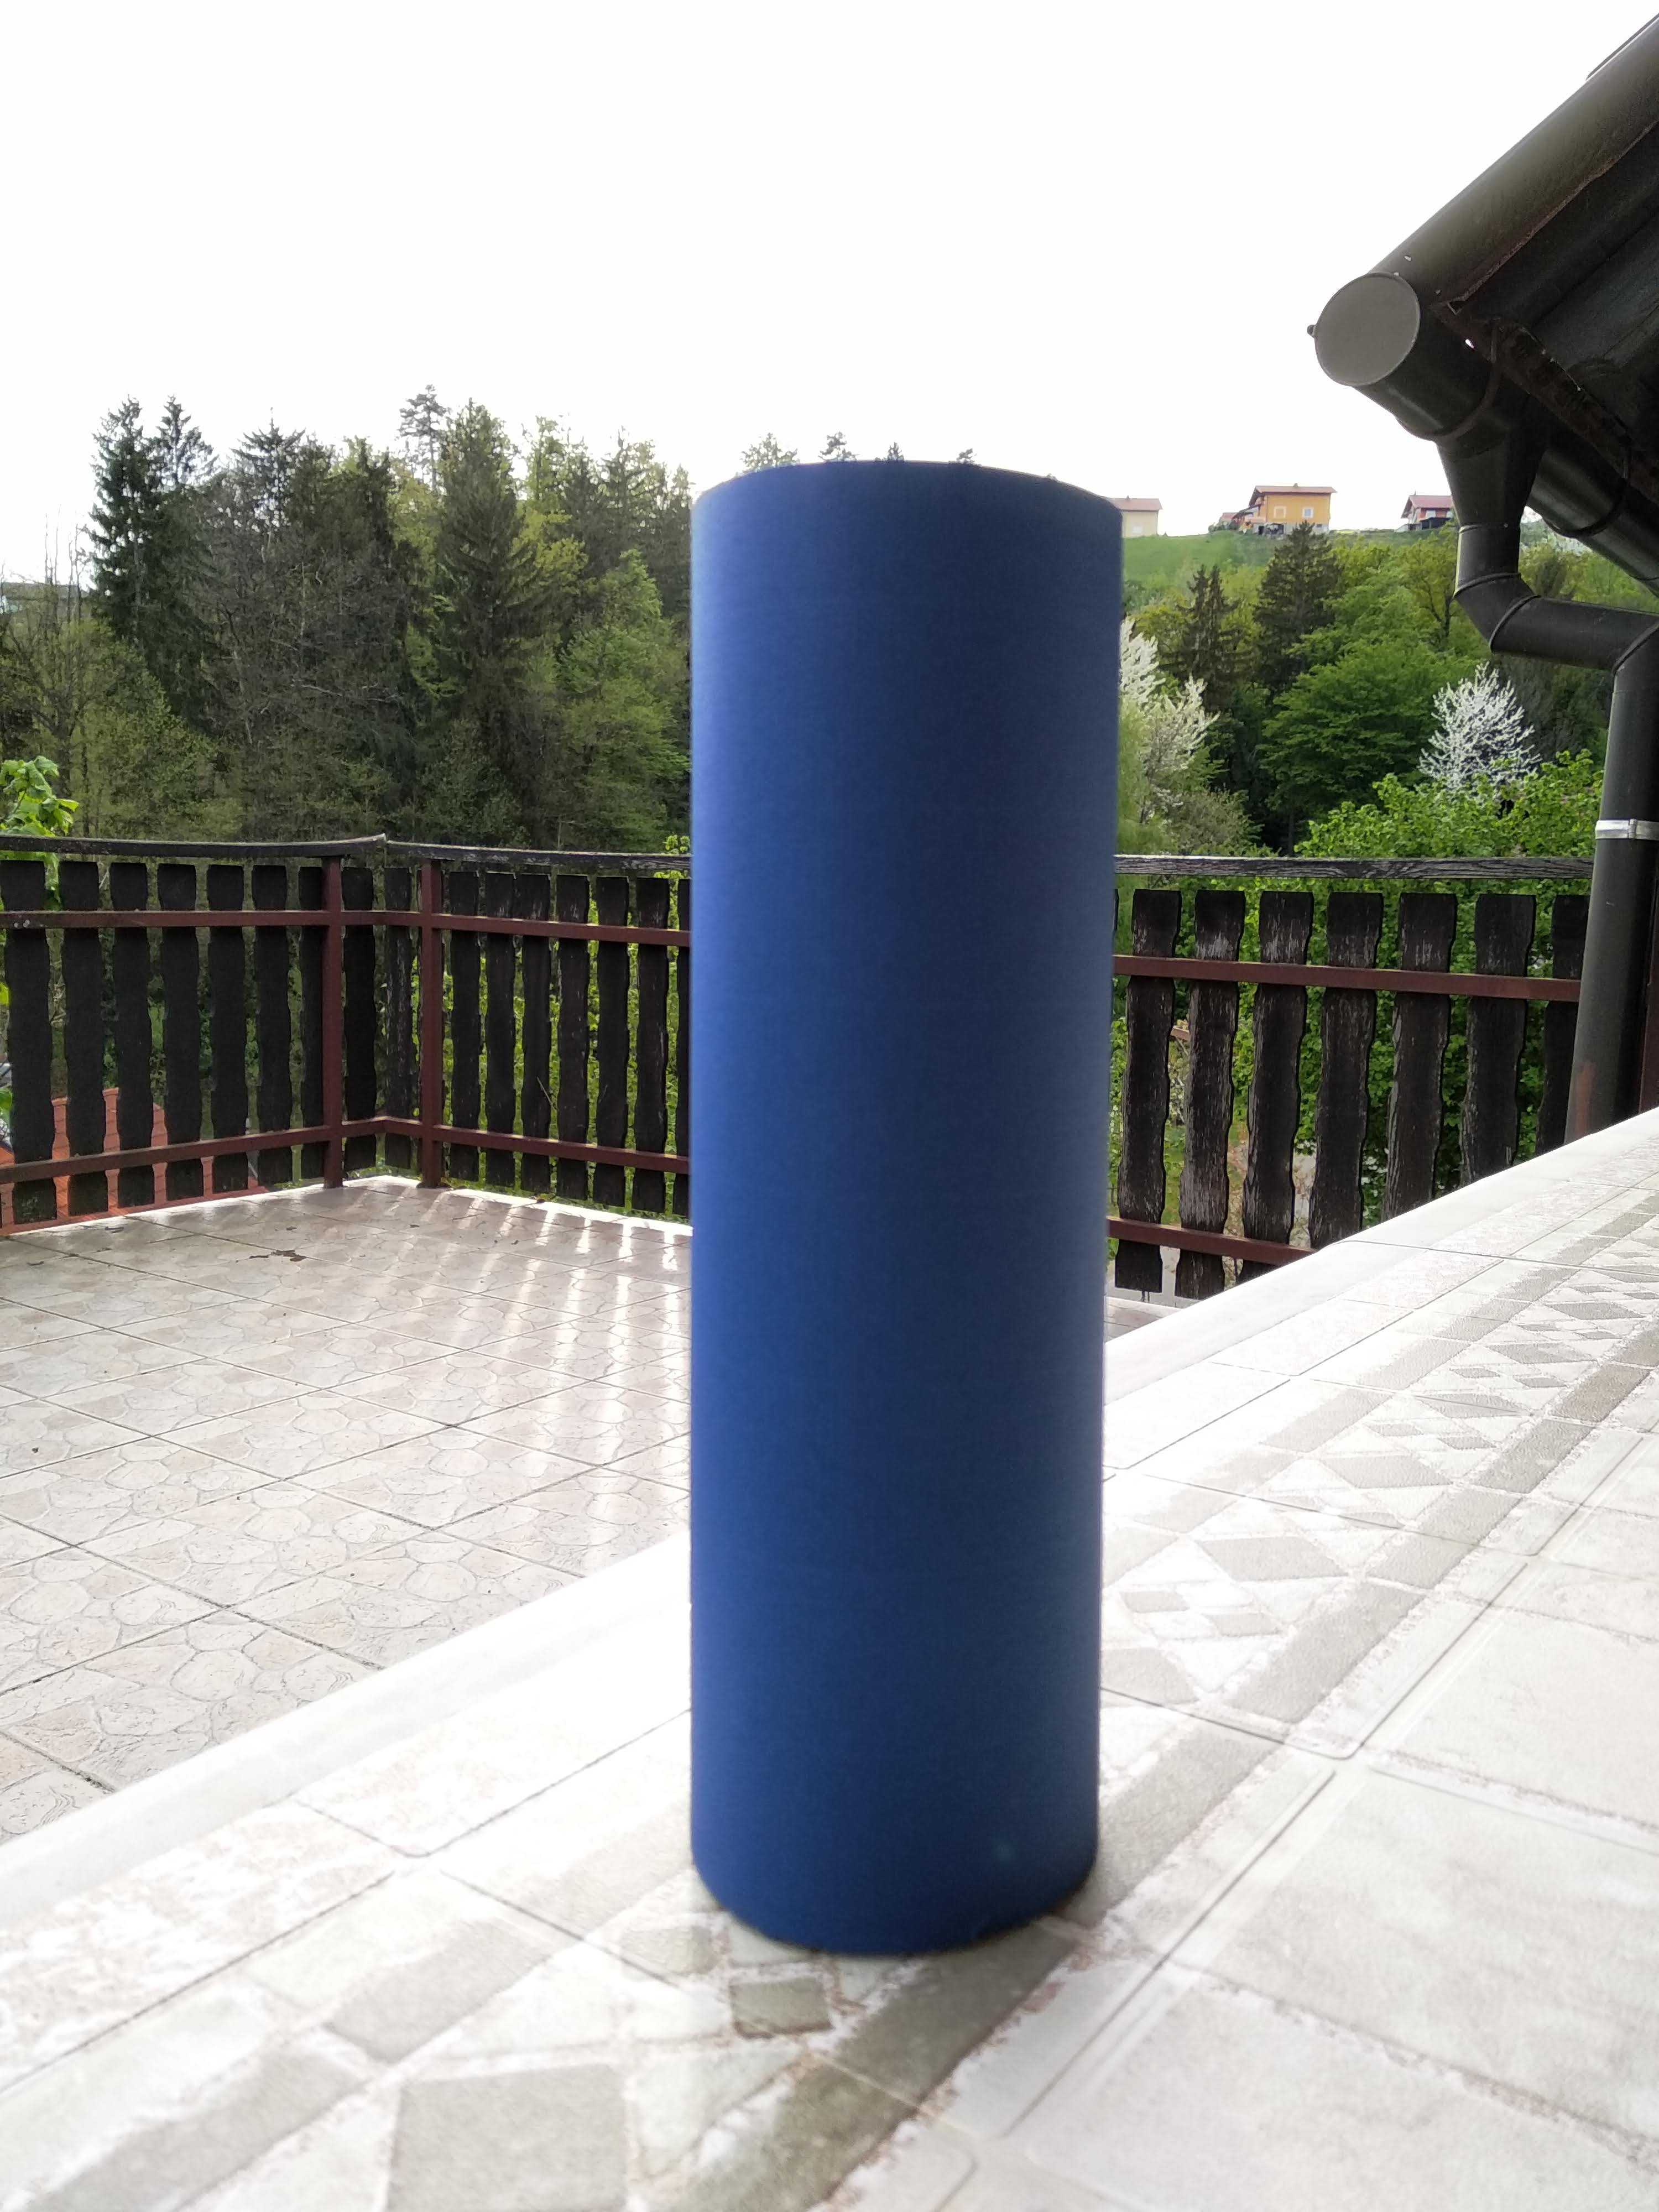
\includegraphics[width=.13\linewidth]{images/test04.jpg}
		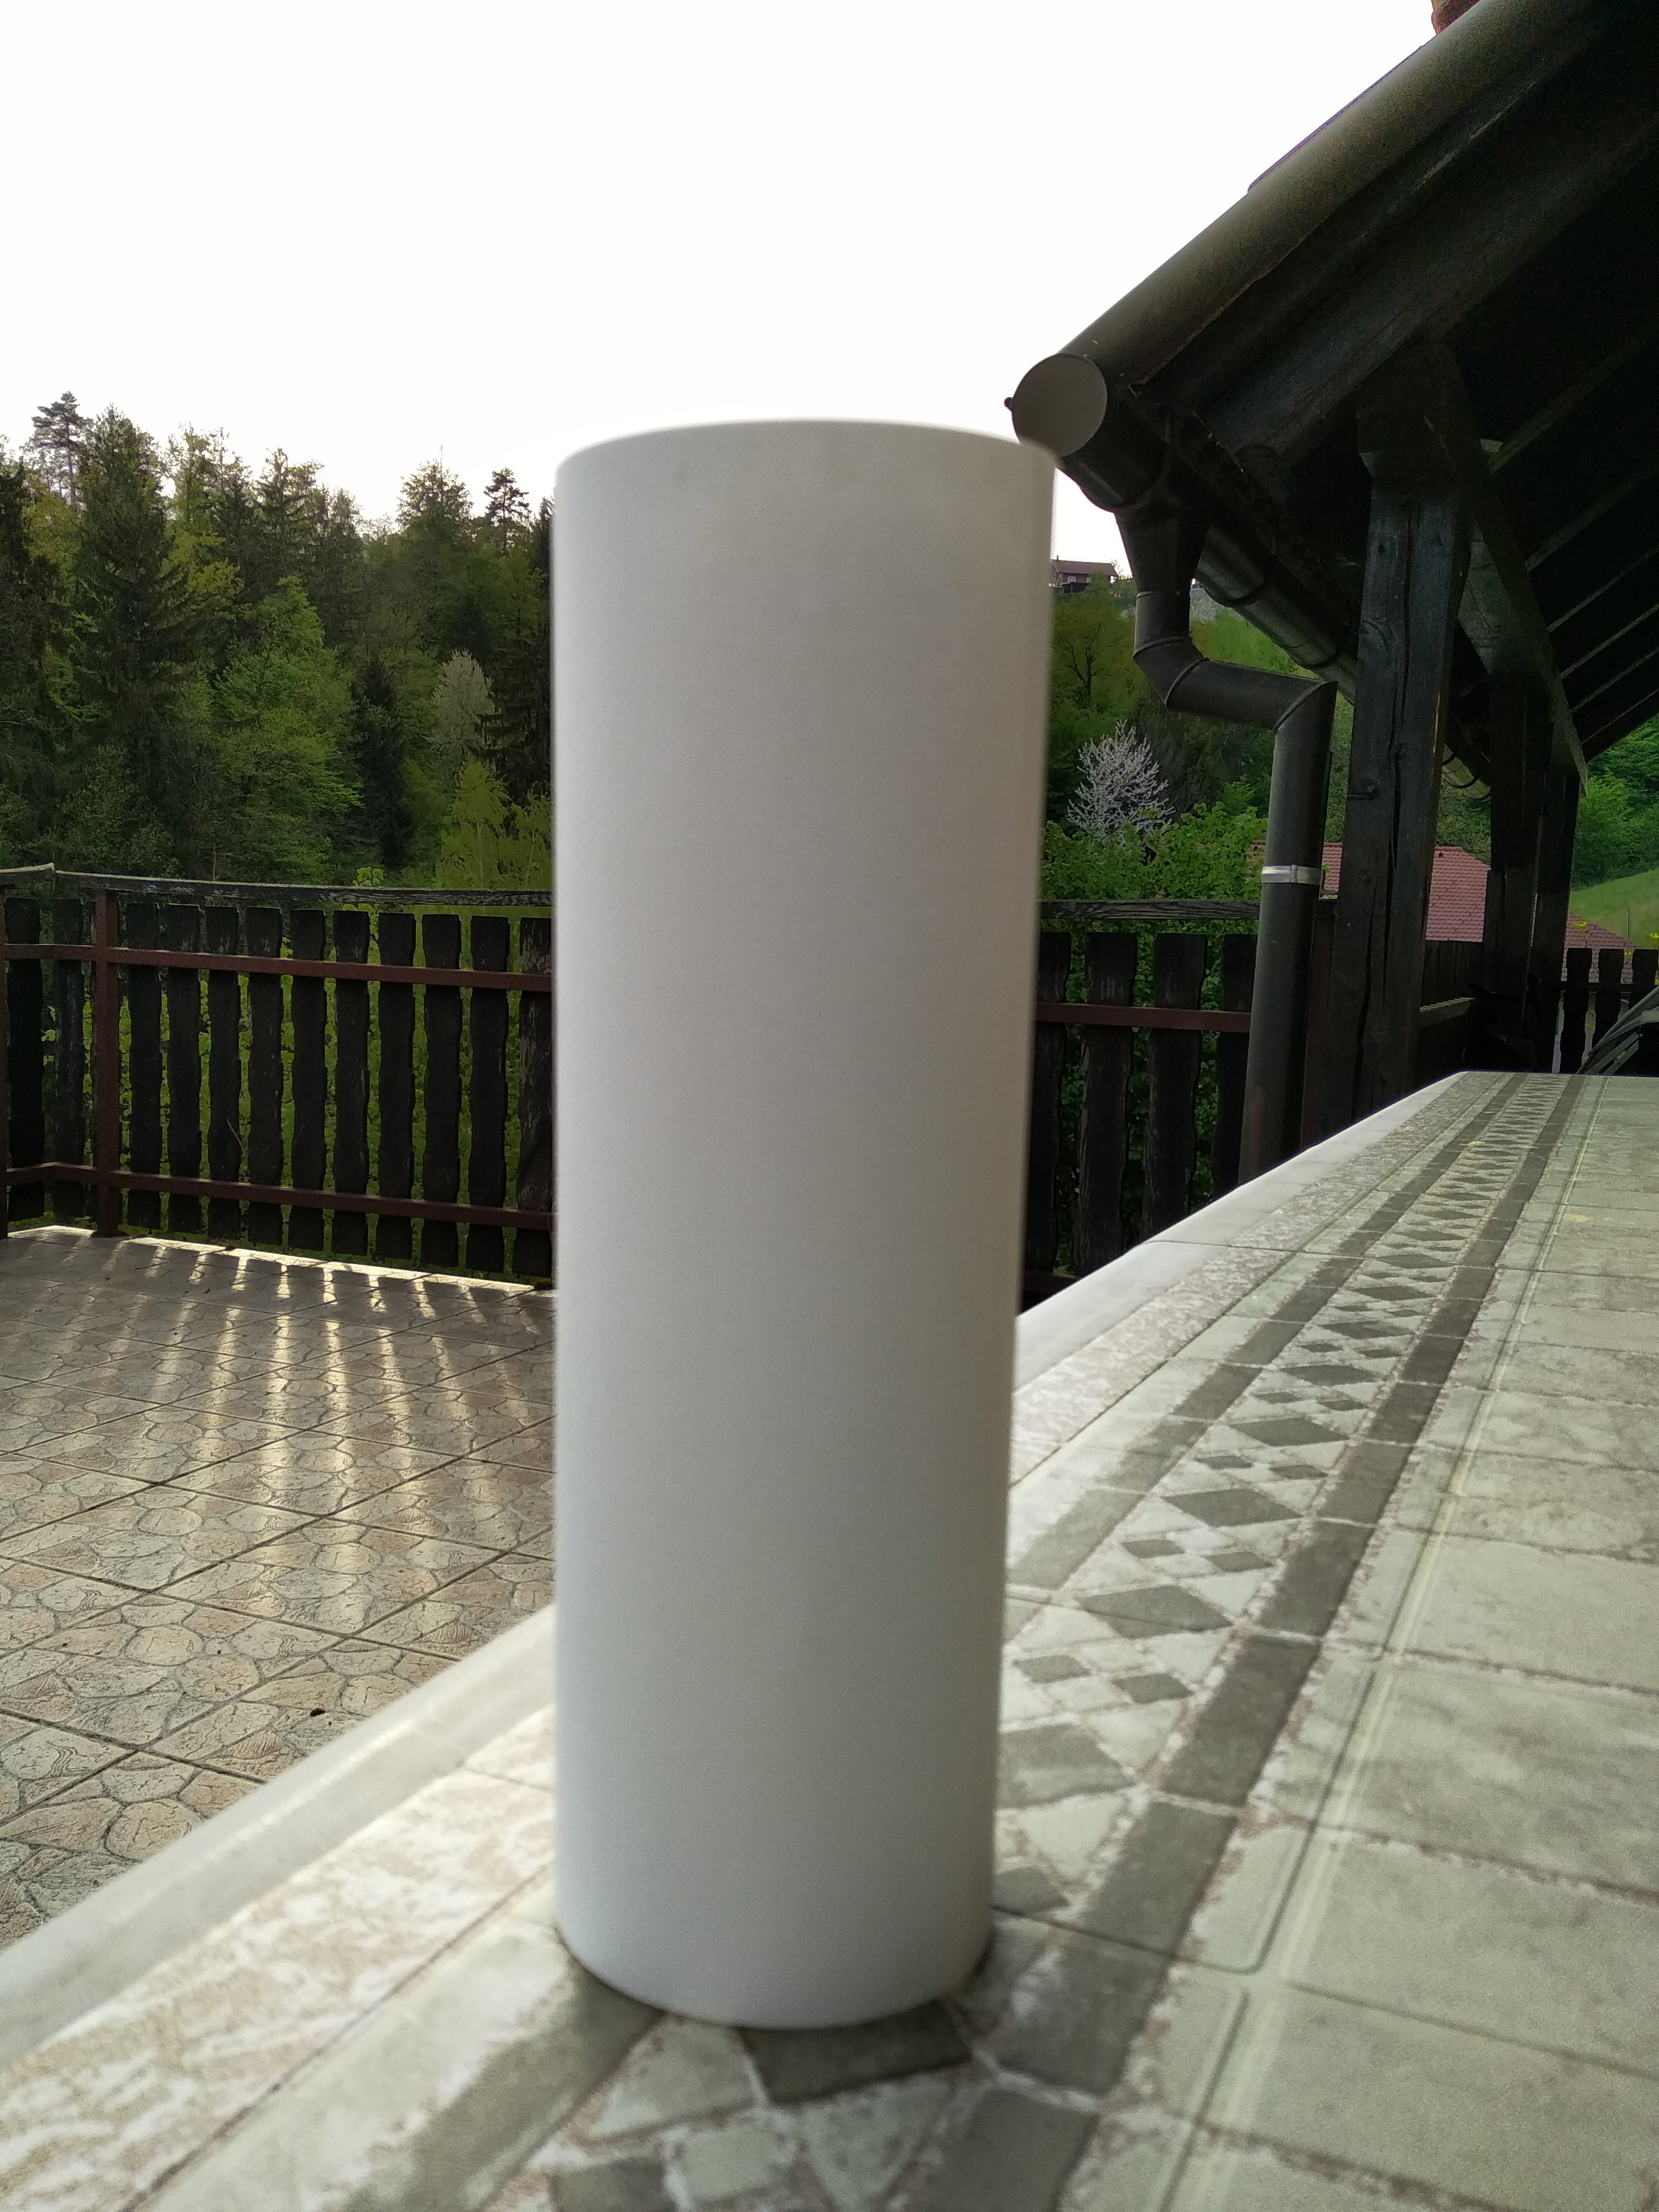
\includegraphics[width=.13\linewidth]{images/test05.jpg}
		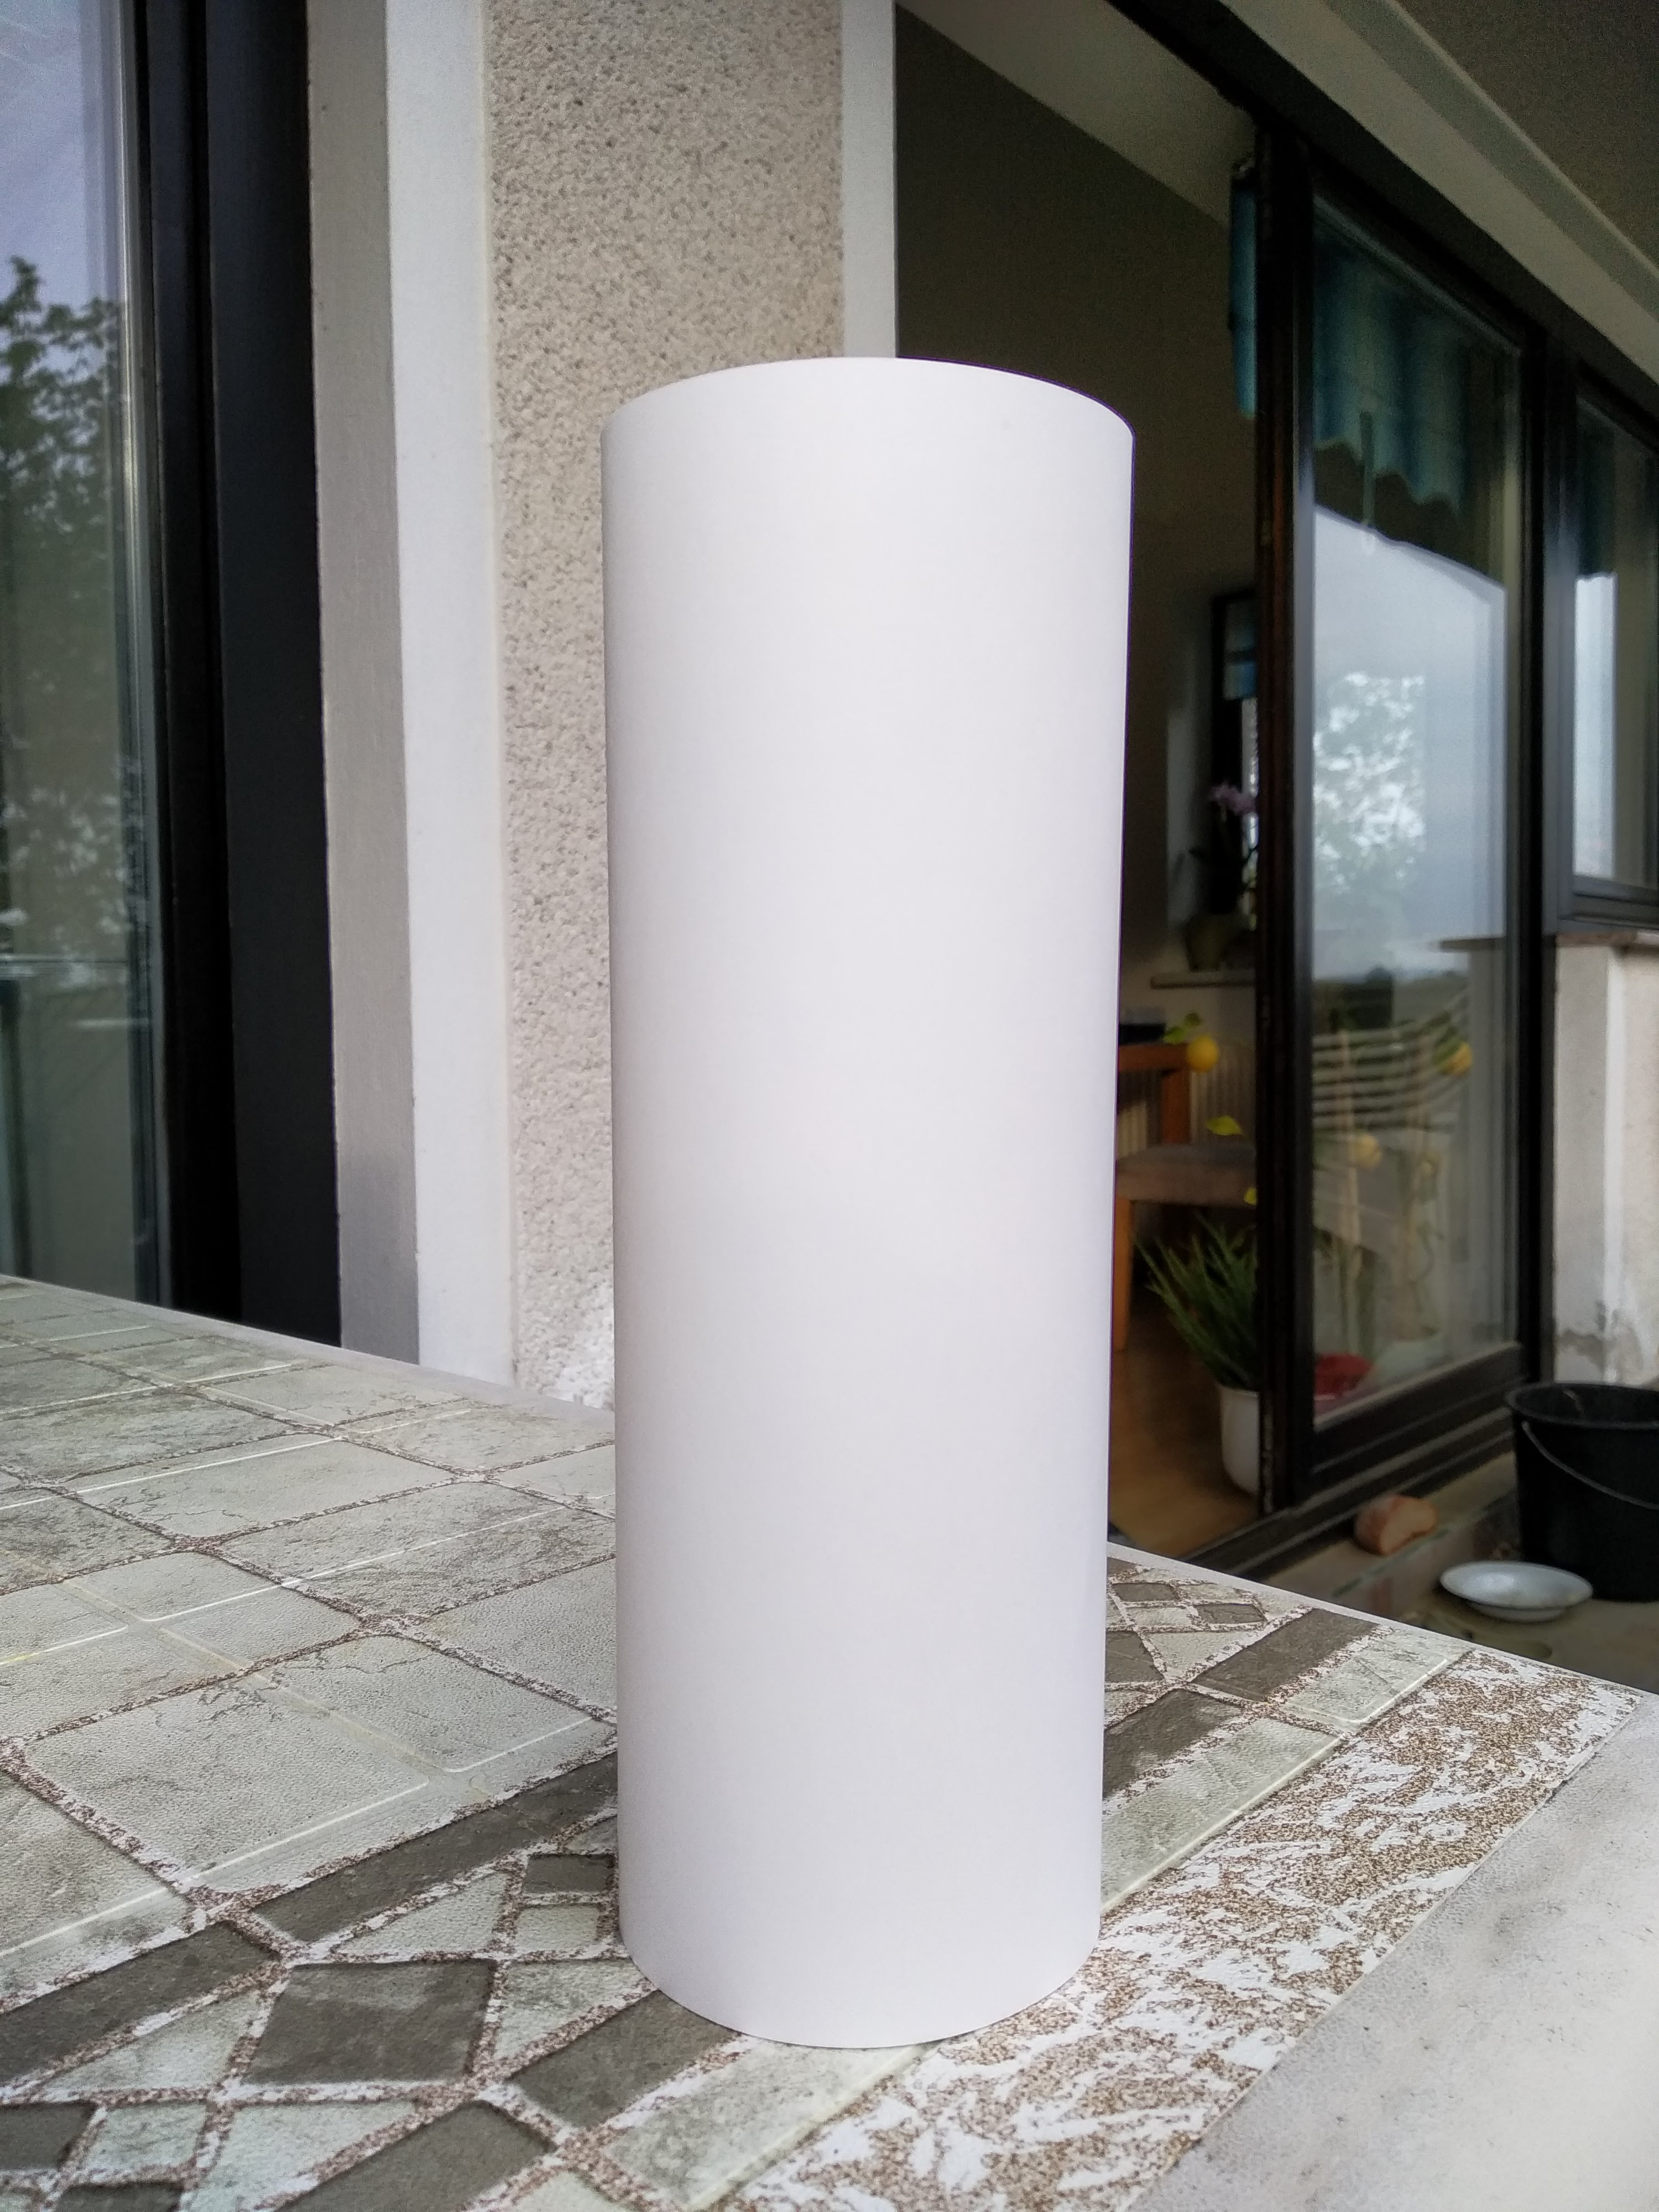
\includegraphics[width=.13\linewidth]{images/test06.jpg} \\
		\vspace{3pt}
		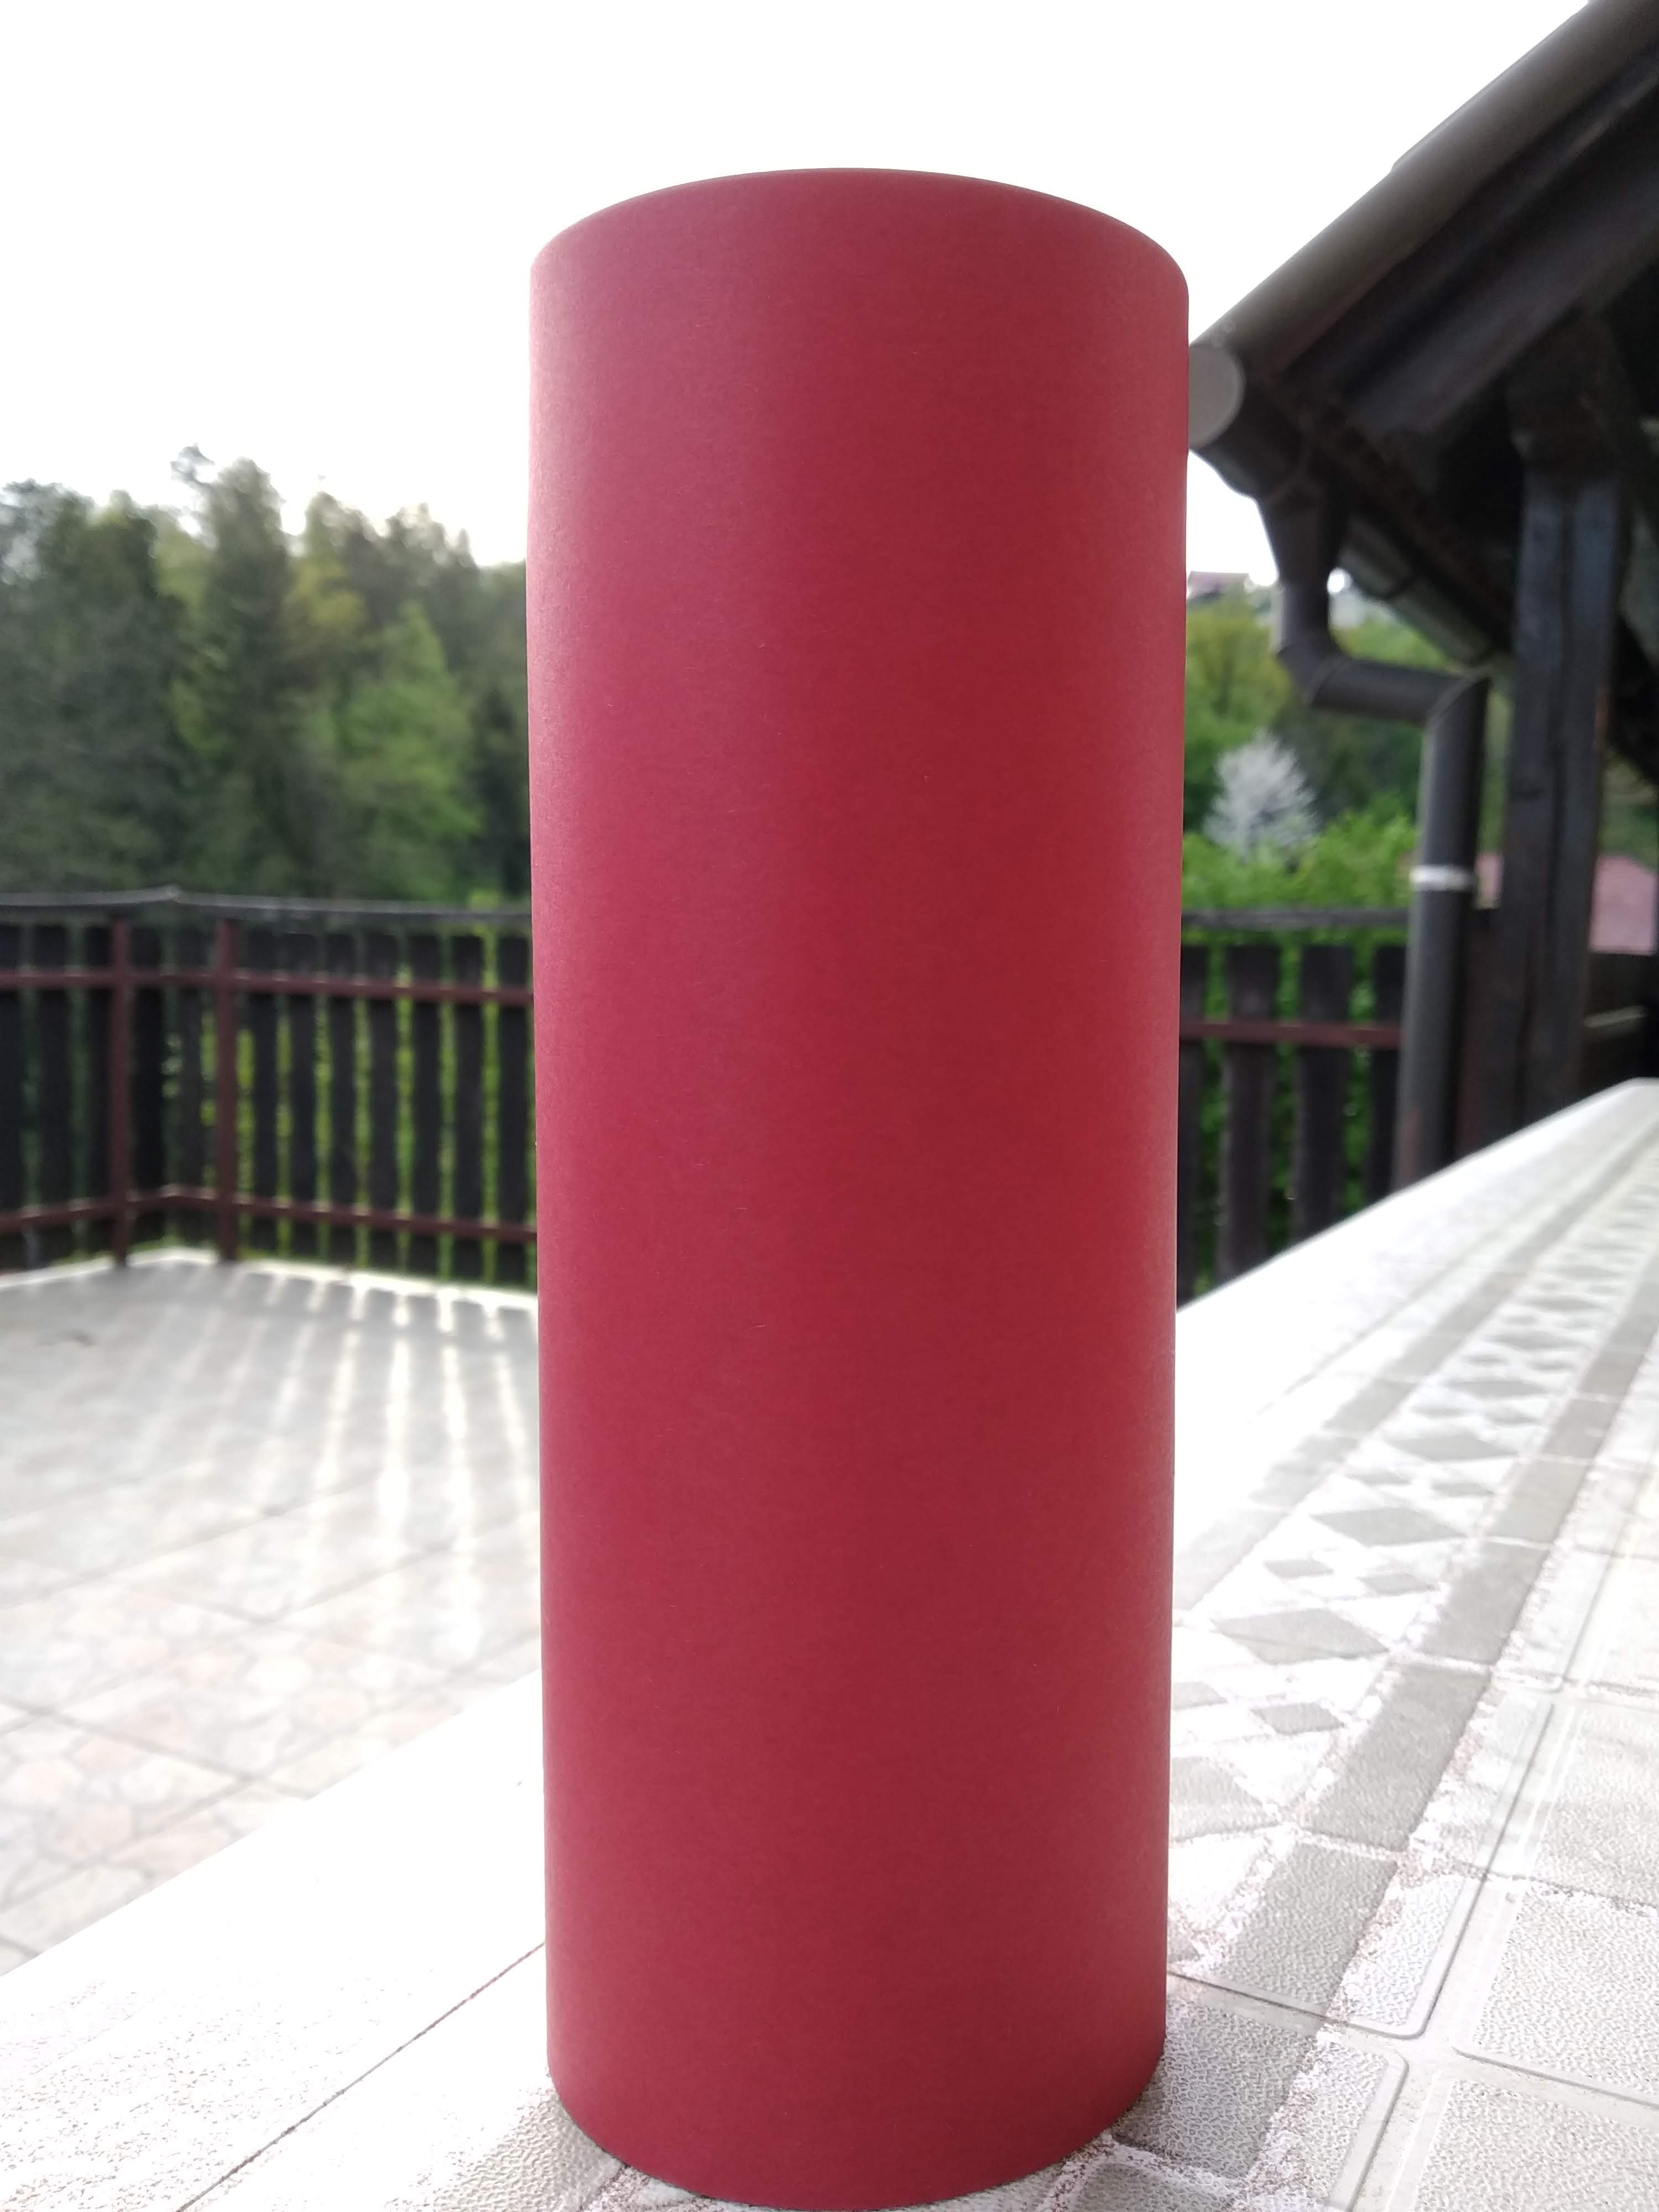
\includegraphics[width=.13\linewidth]{images/test07.jpg}
		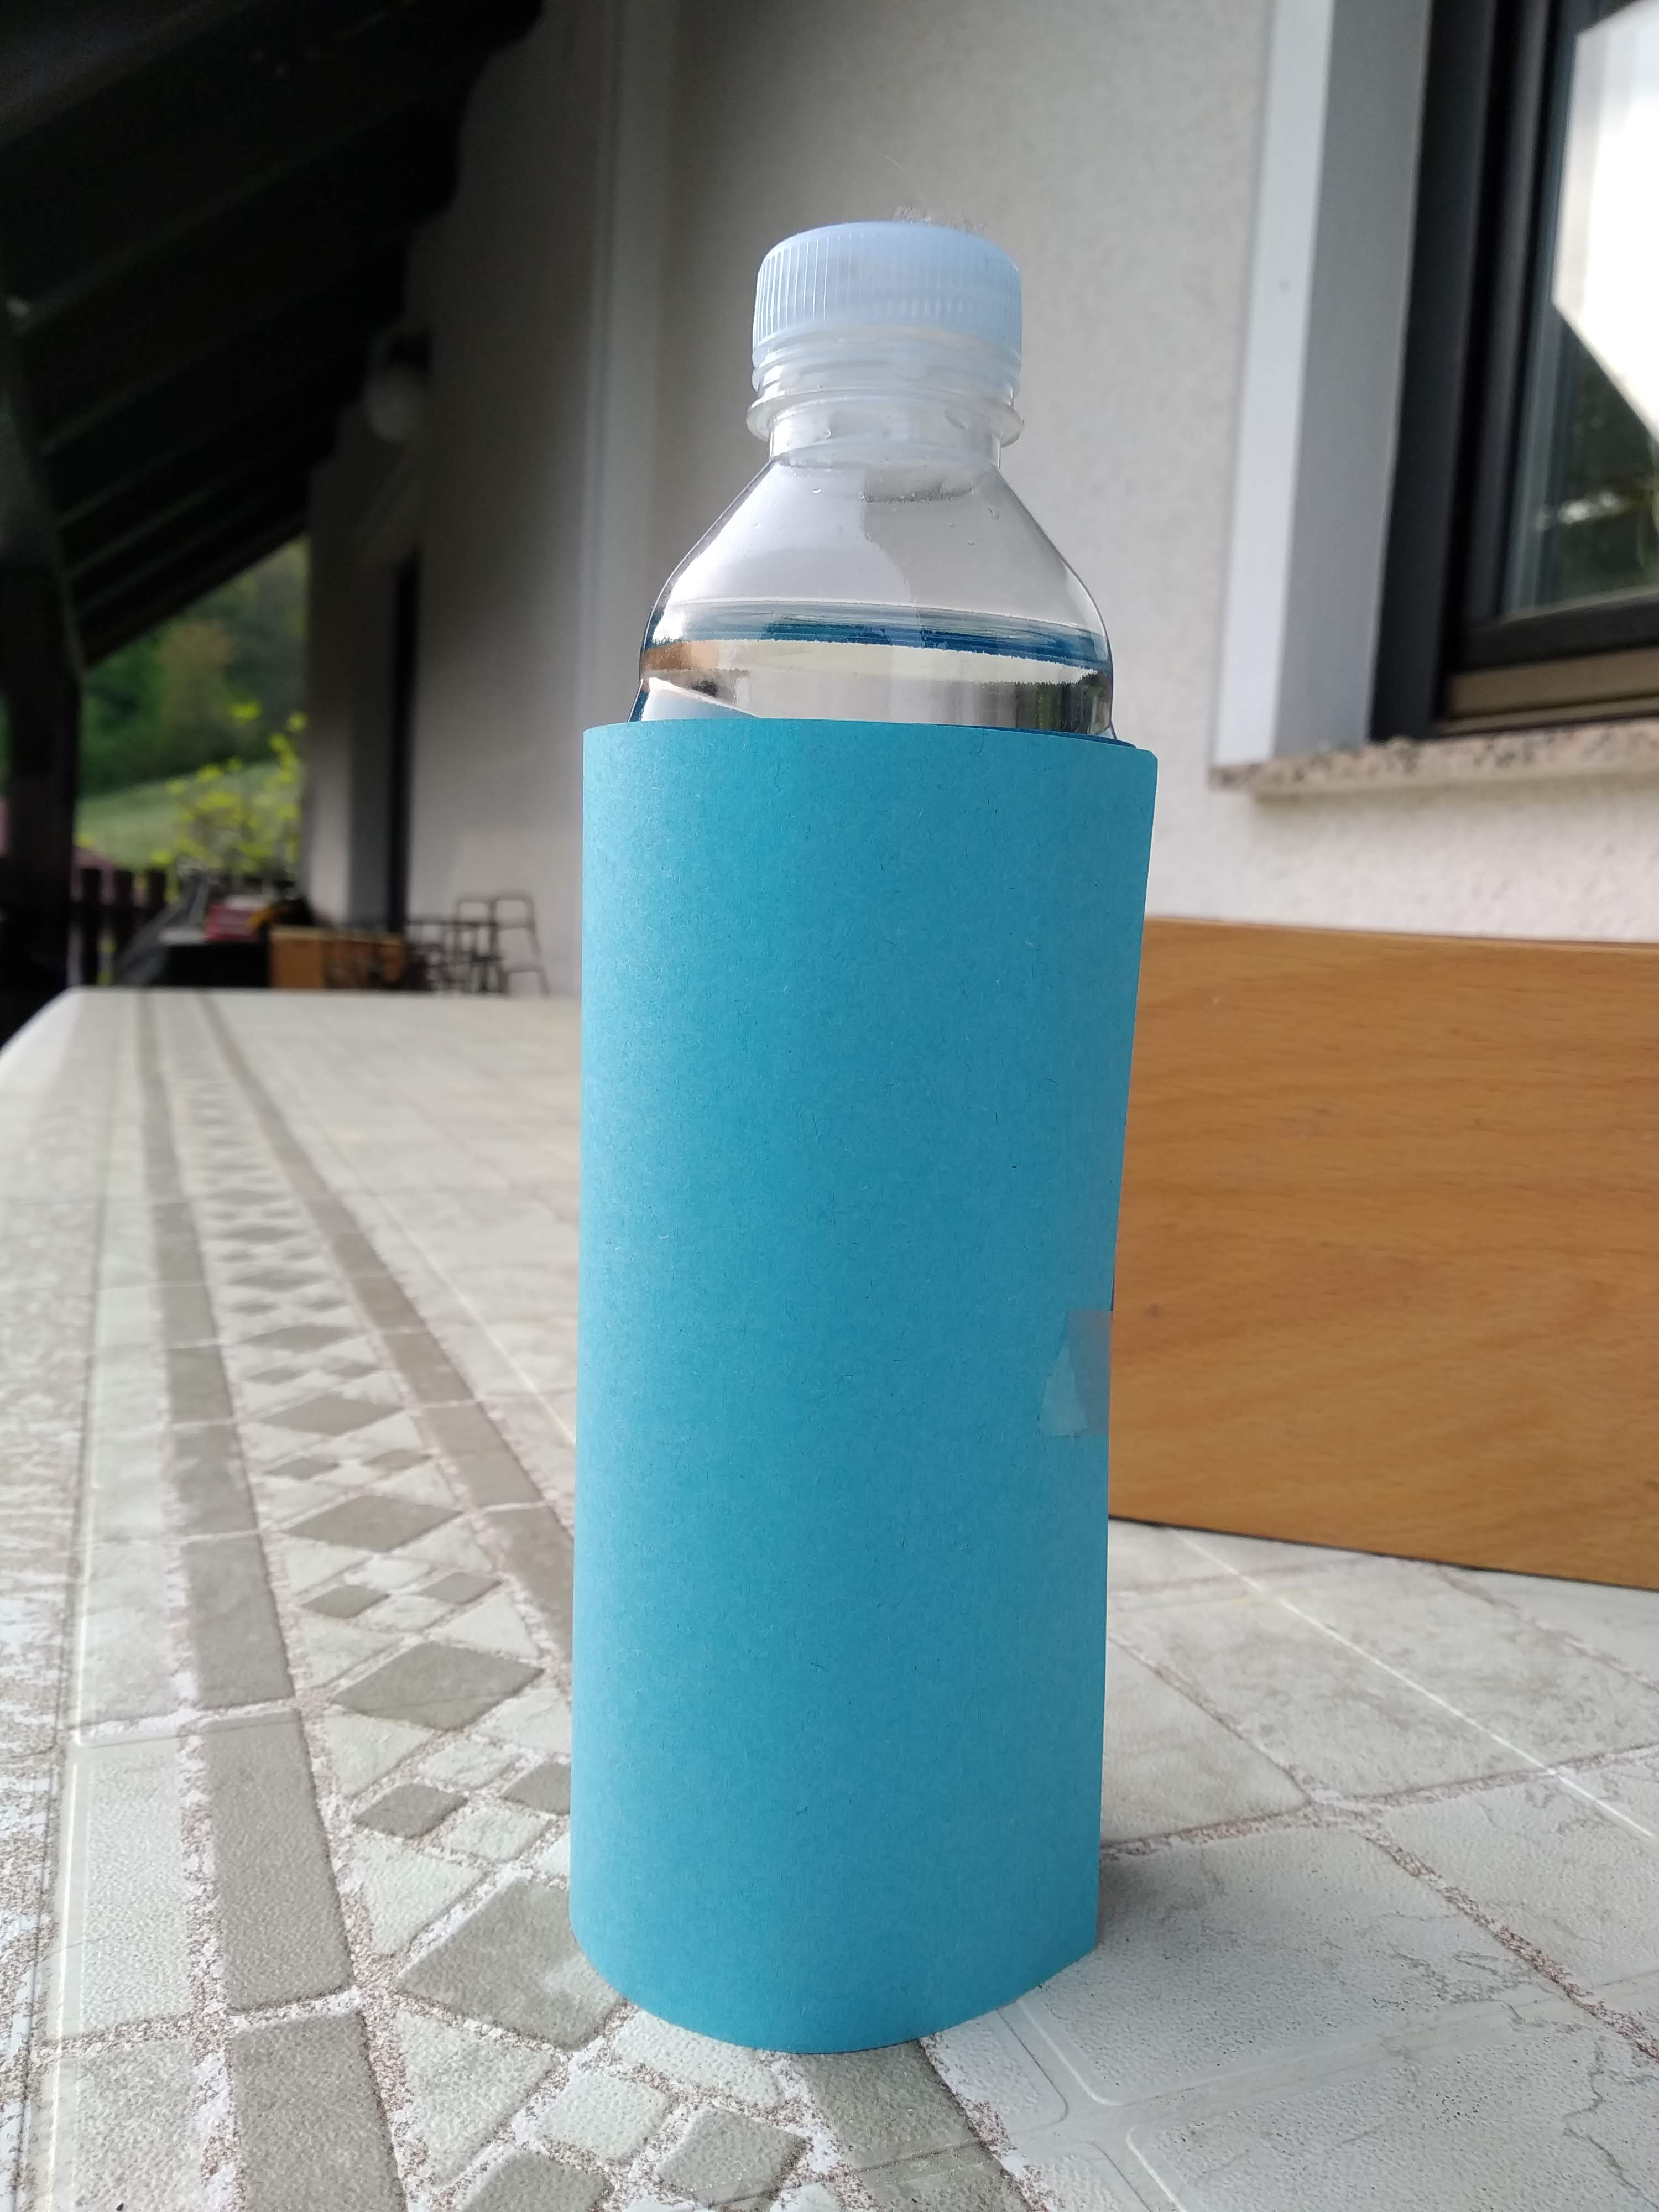
\includegraphics[width=.13\linewidth]{images/test08.jpg}
		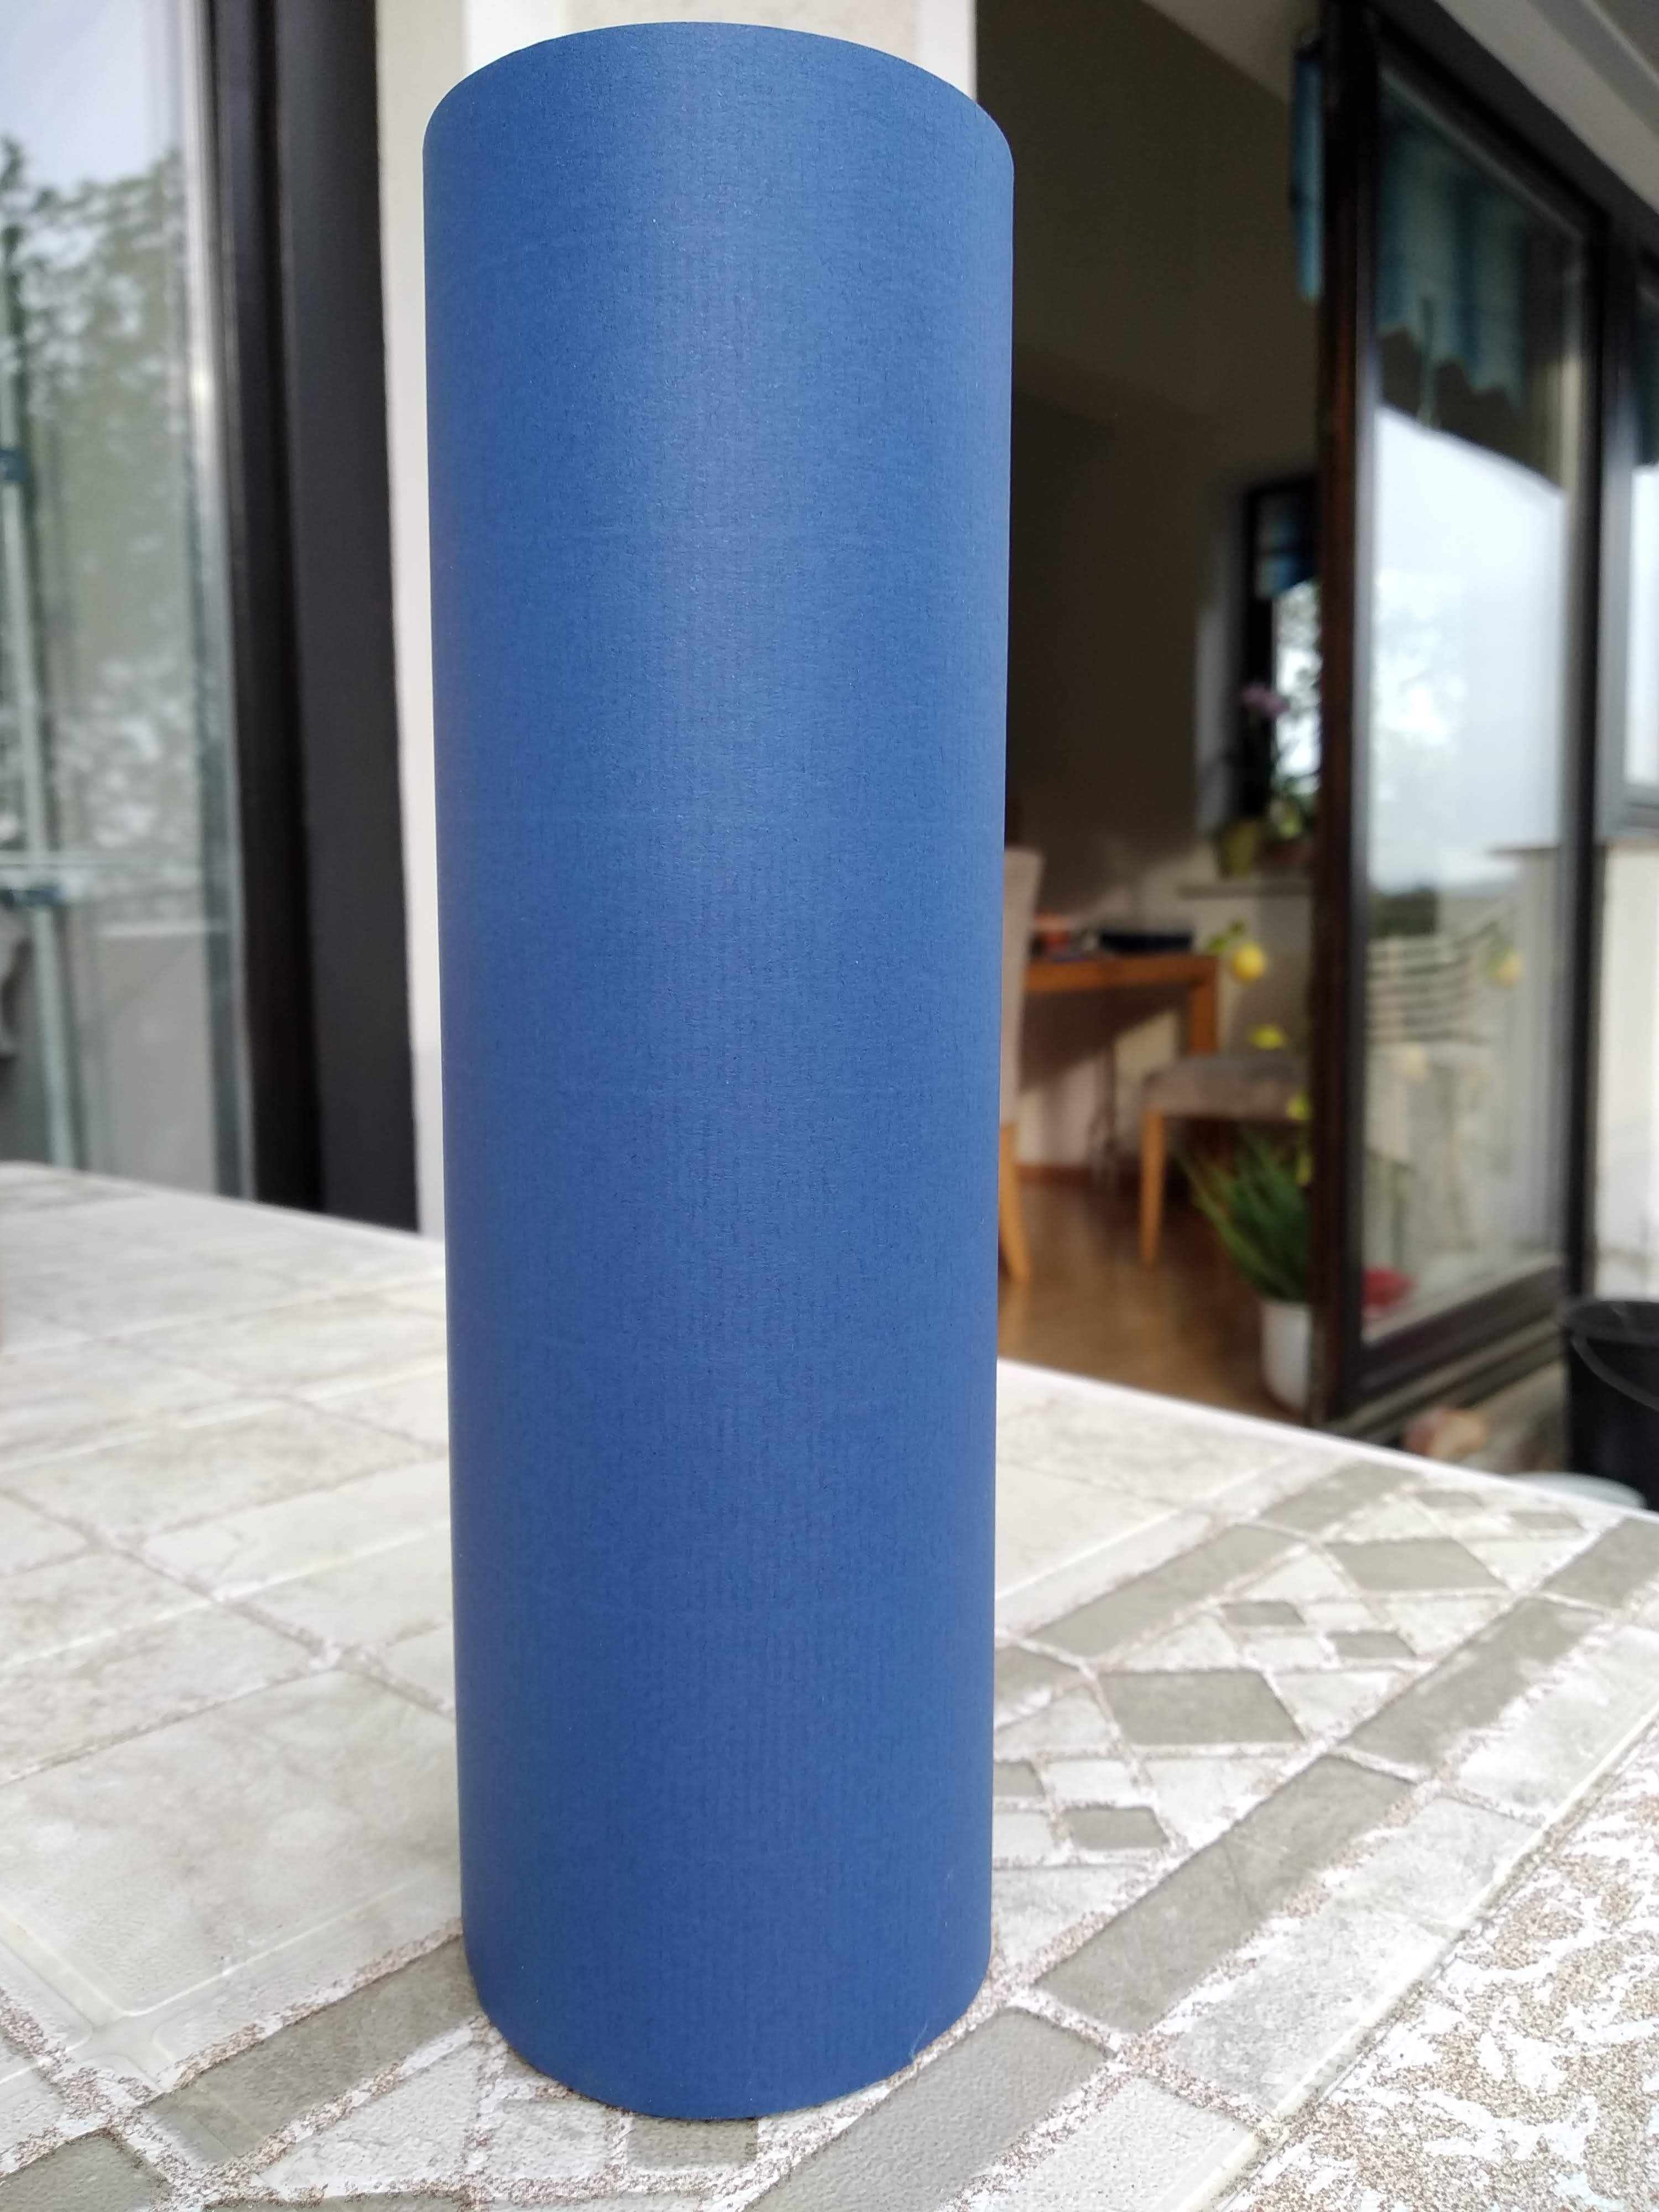
\includegraphics[width=.13\linewidth]{images/test_09_remove_if_too_many_photos.jpg}
		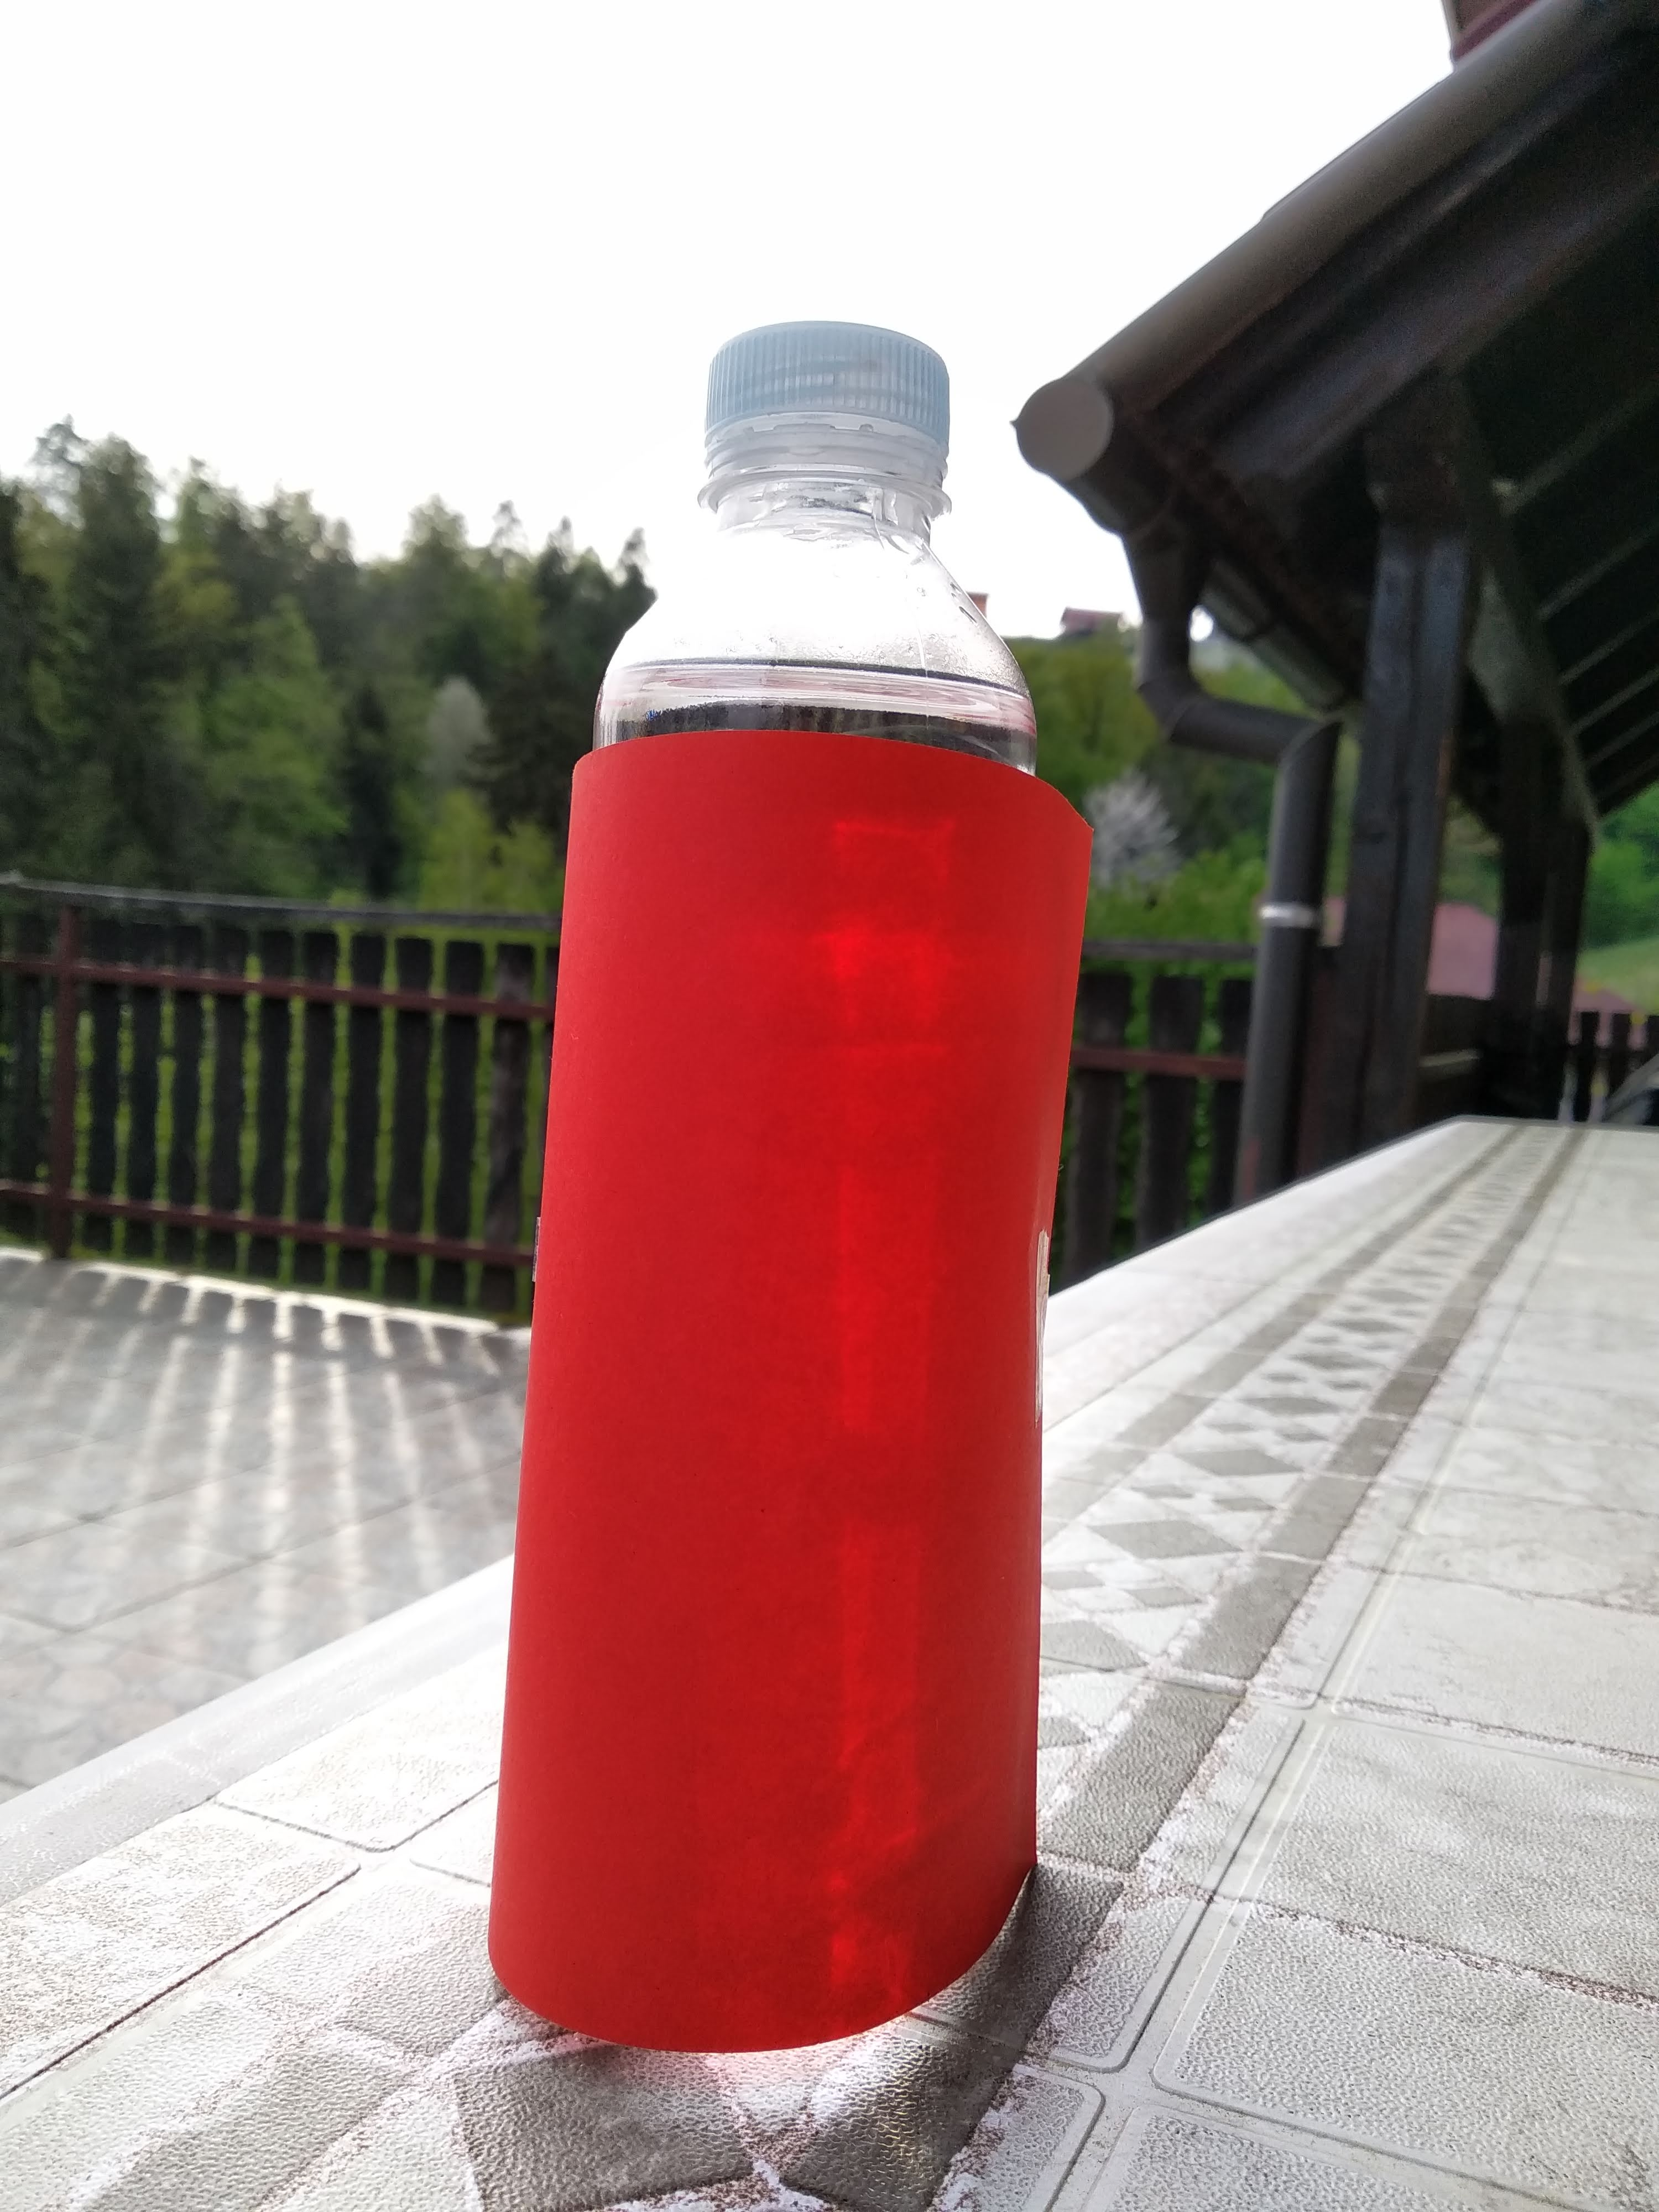
\includegraphics[width=.13\linewidth]{images/test_10_remove_if_too_many_photos.jpg}
		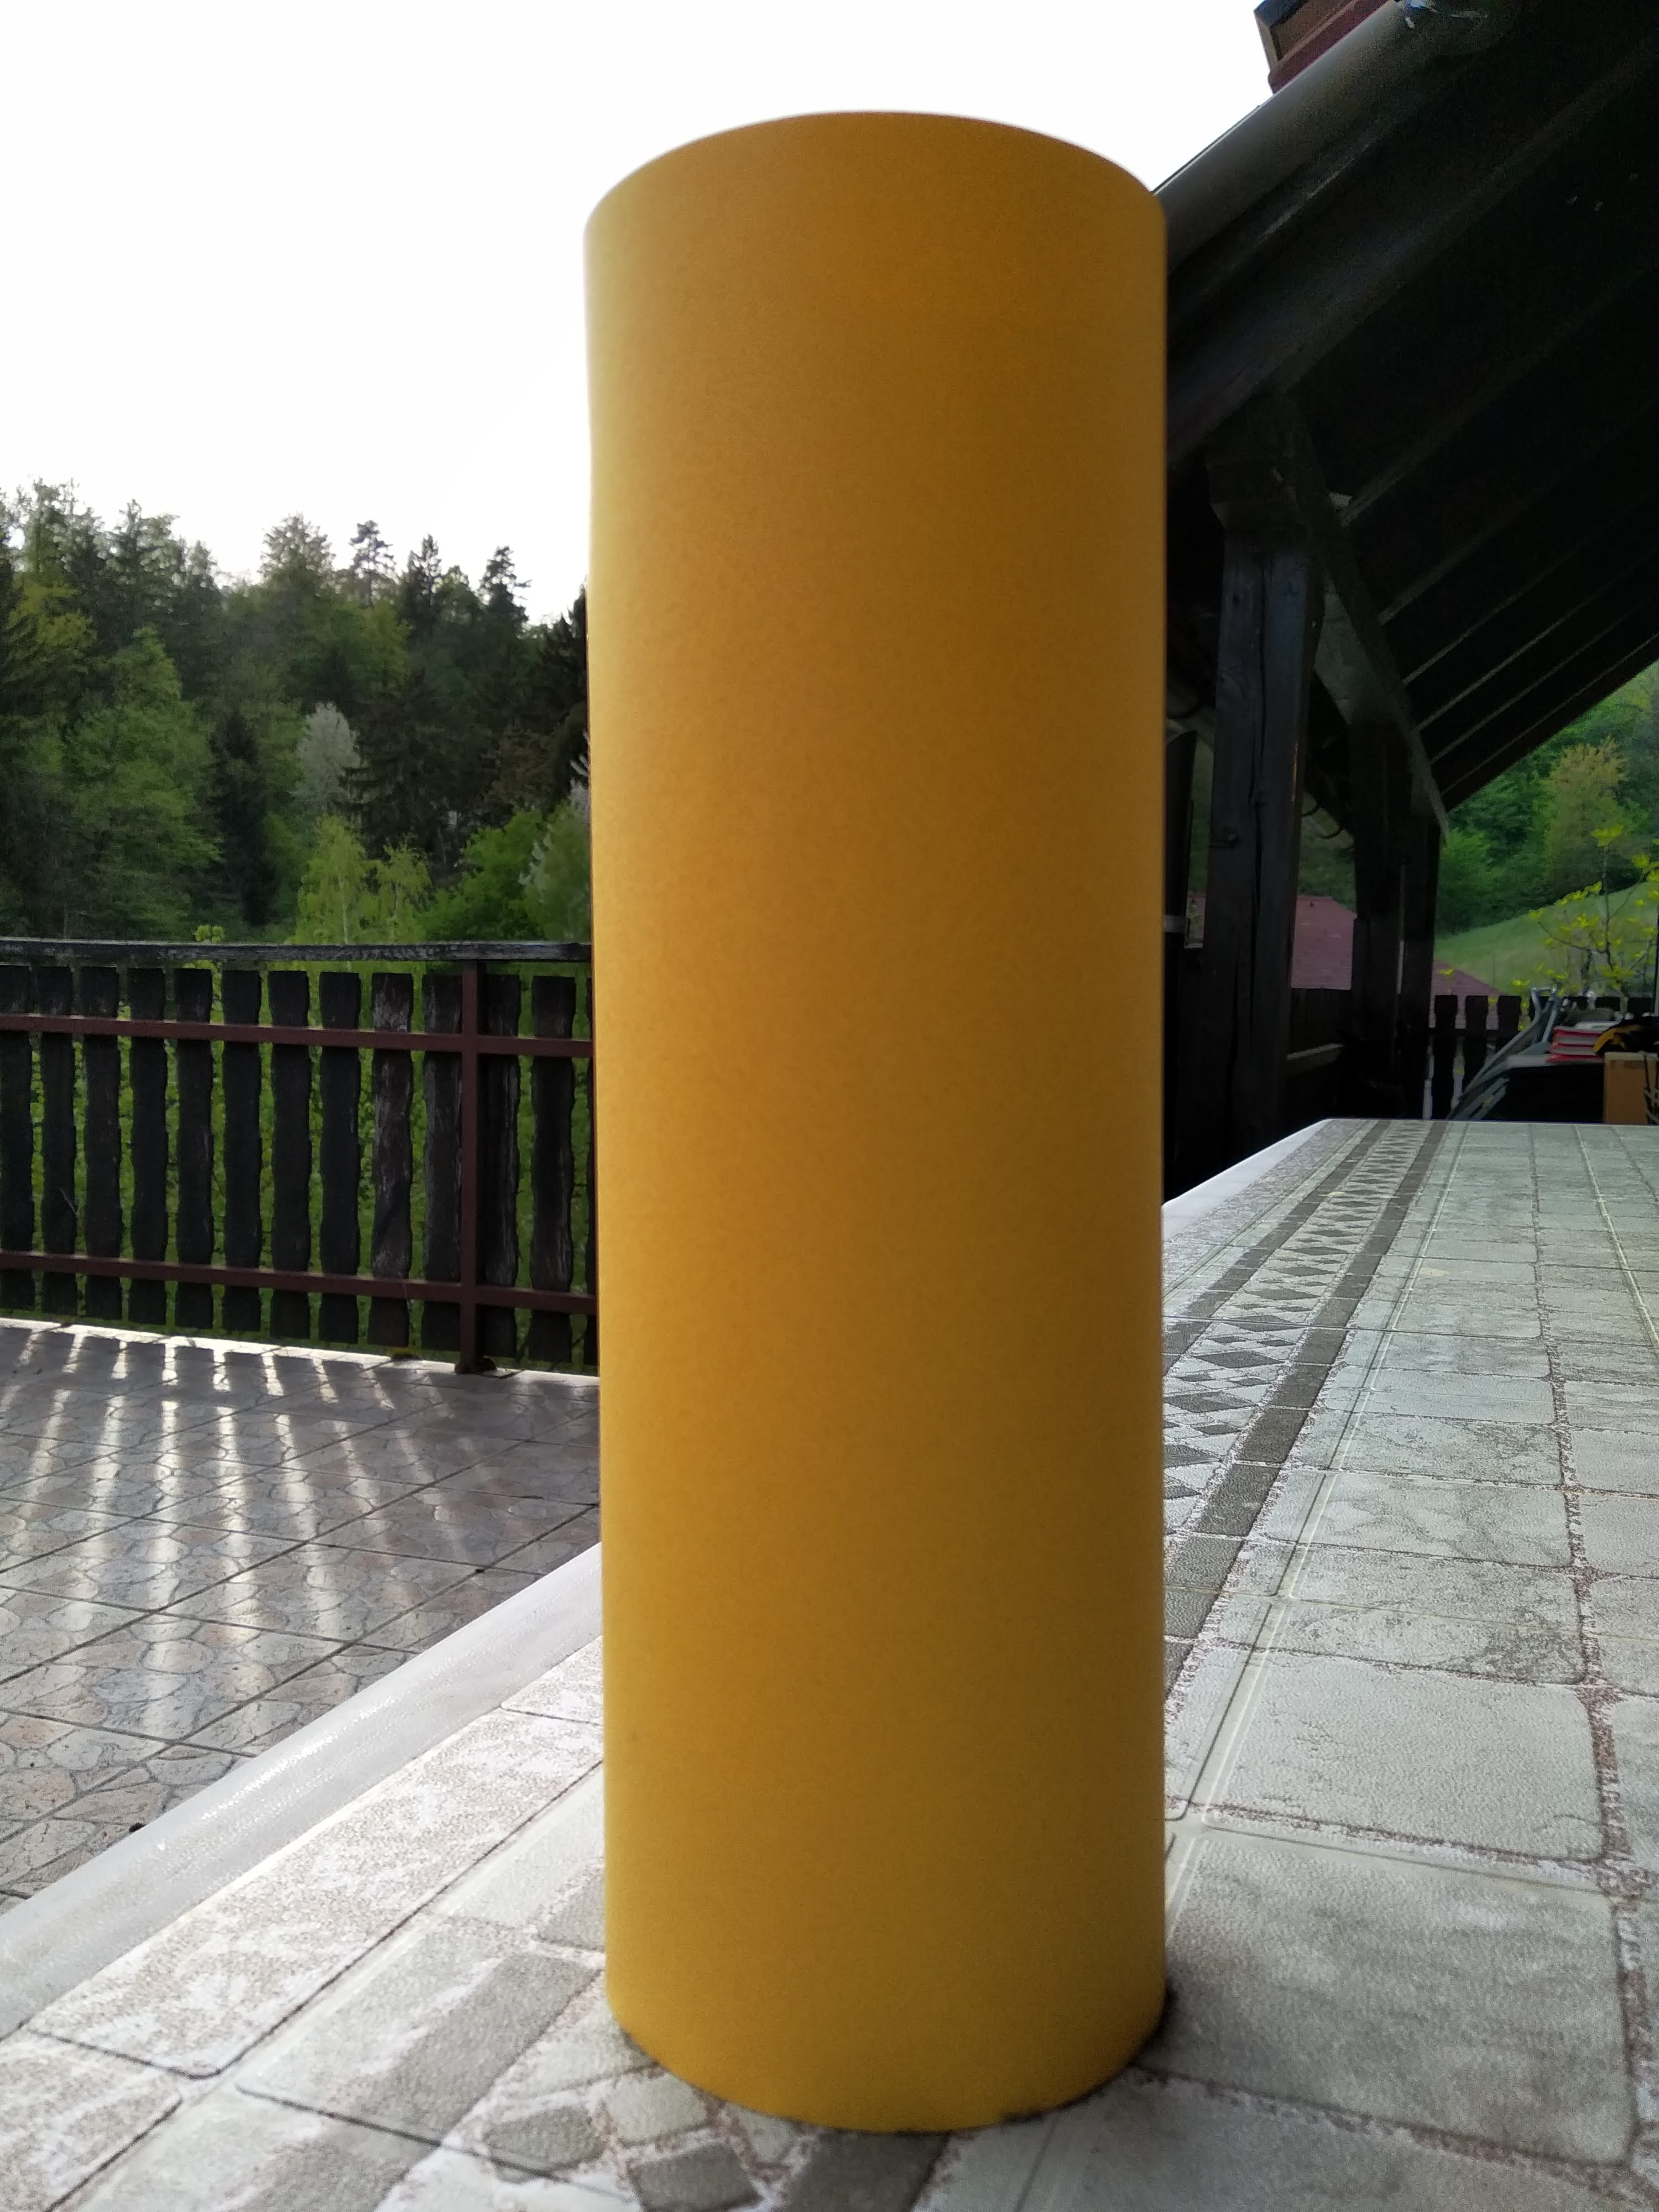
\includegraphics[width=.13\linewidth]{images/test_11_remove_if_too_many_photos.jpg}
		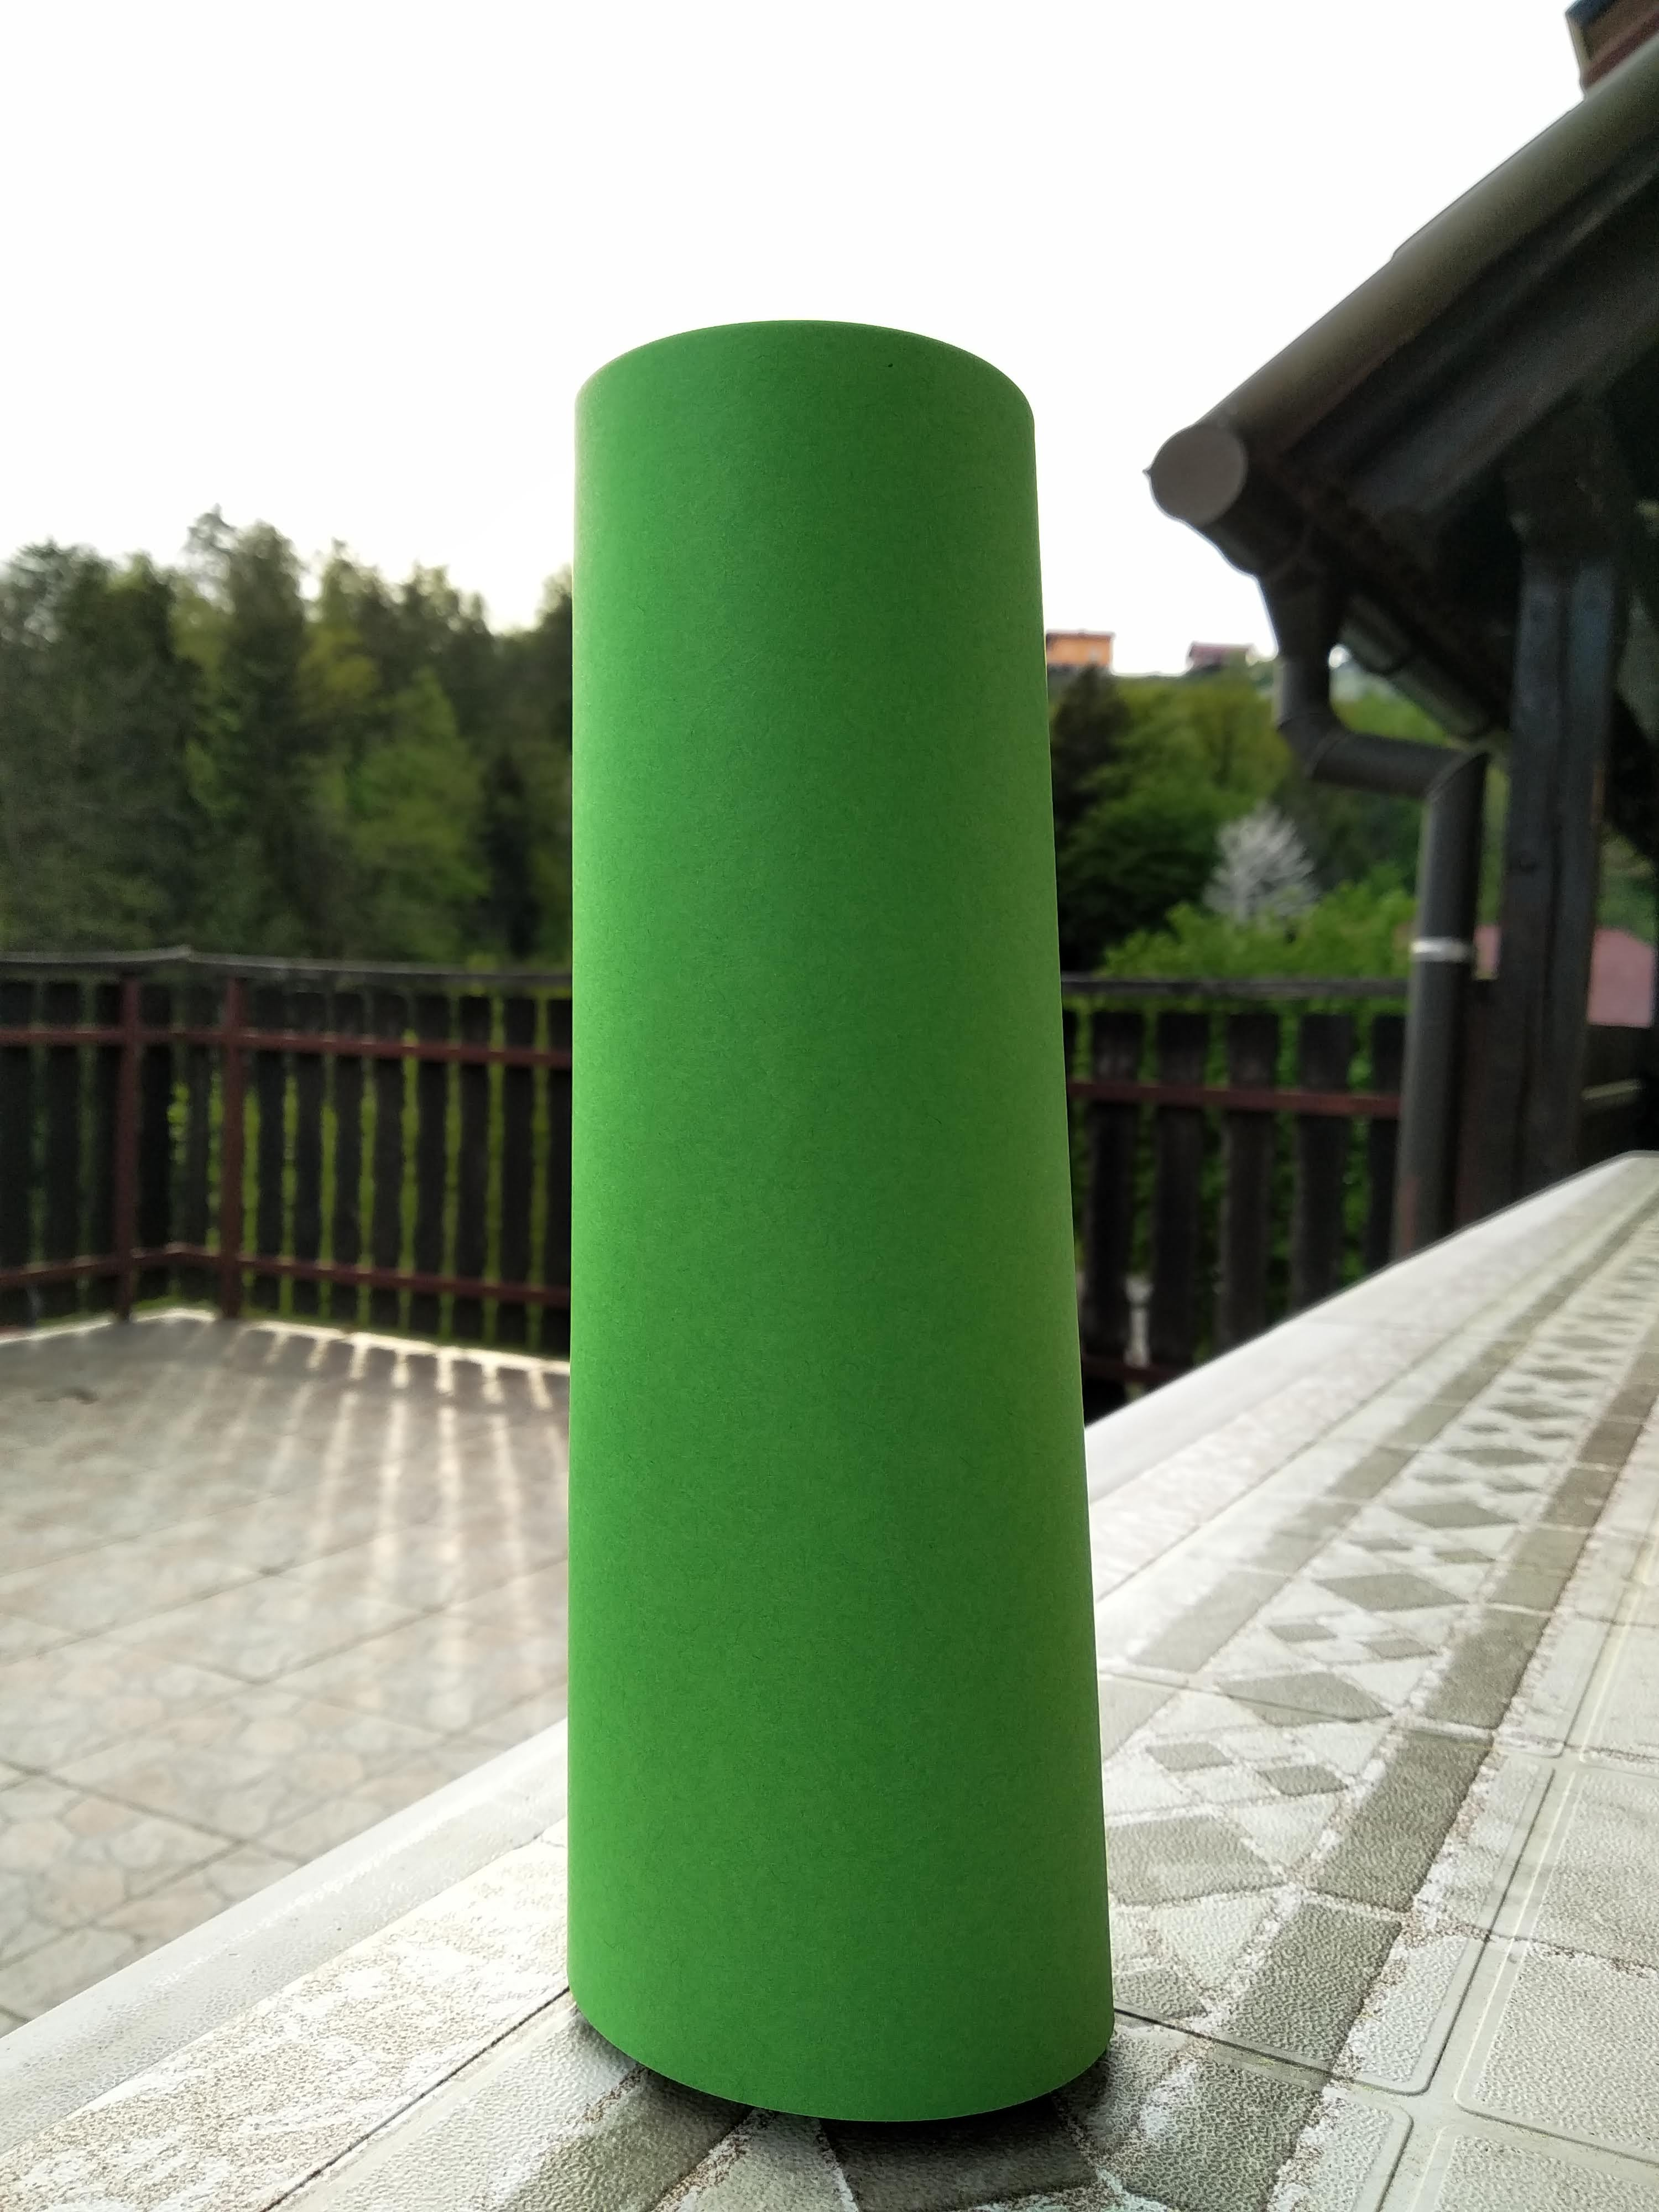
\includegraphics[width=.13\linewidth]{images/test_12_remove_if_too_many_photos.jpg}
		\caption{Second set of photos}
	\end{figure}

	\subsection{Preprocessing photos}

	To prepare the images for classifiers, we cropped the circles to perfect circles and cylinders to rectangles. Some examples of cropped cylinders are shown below.

	\begin{figure}[H]
		\centering
		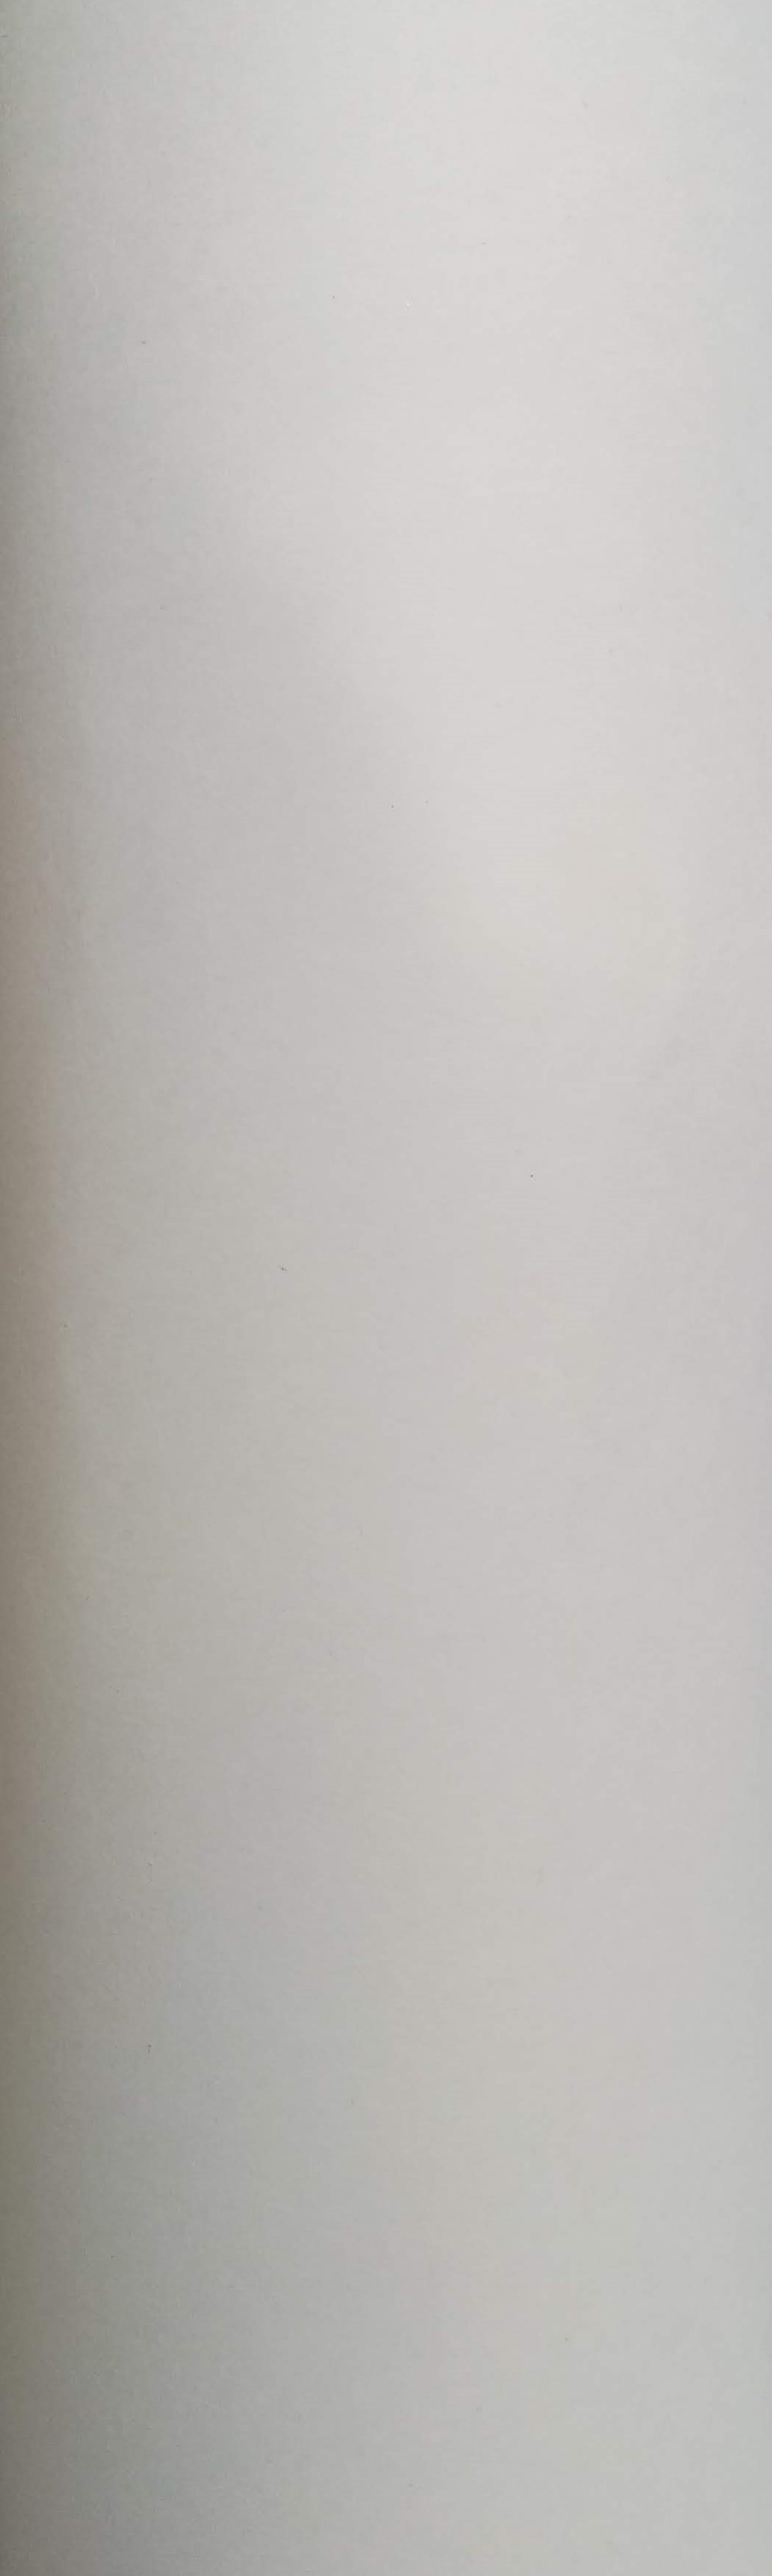
\includegraphics[width=.08\linewidth, height=.08\linewidth]{images/test_cut_01.jpg}
		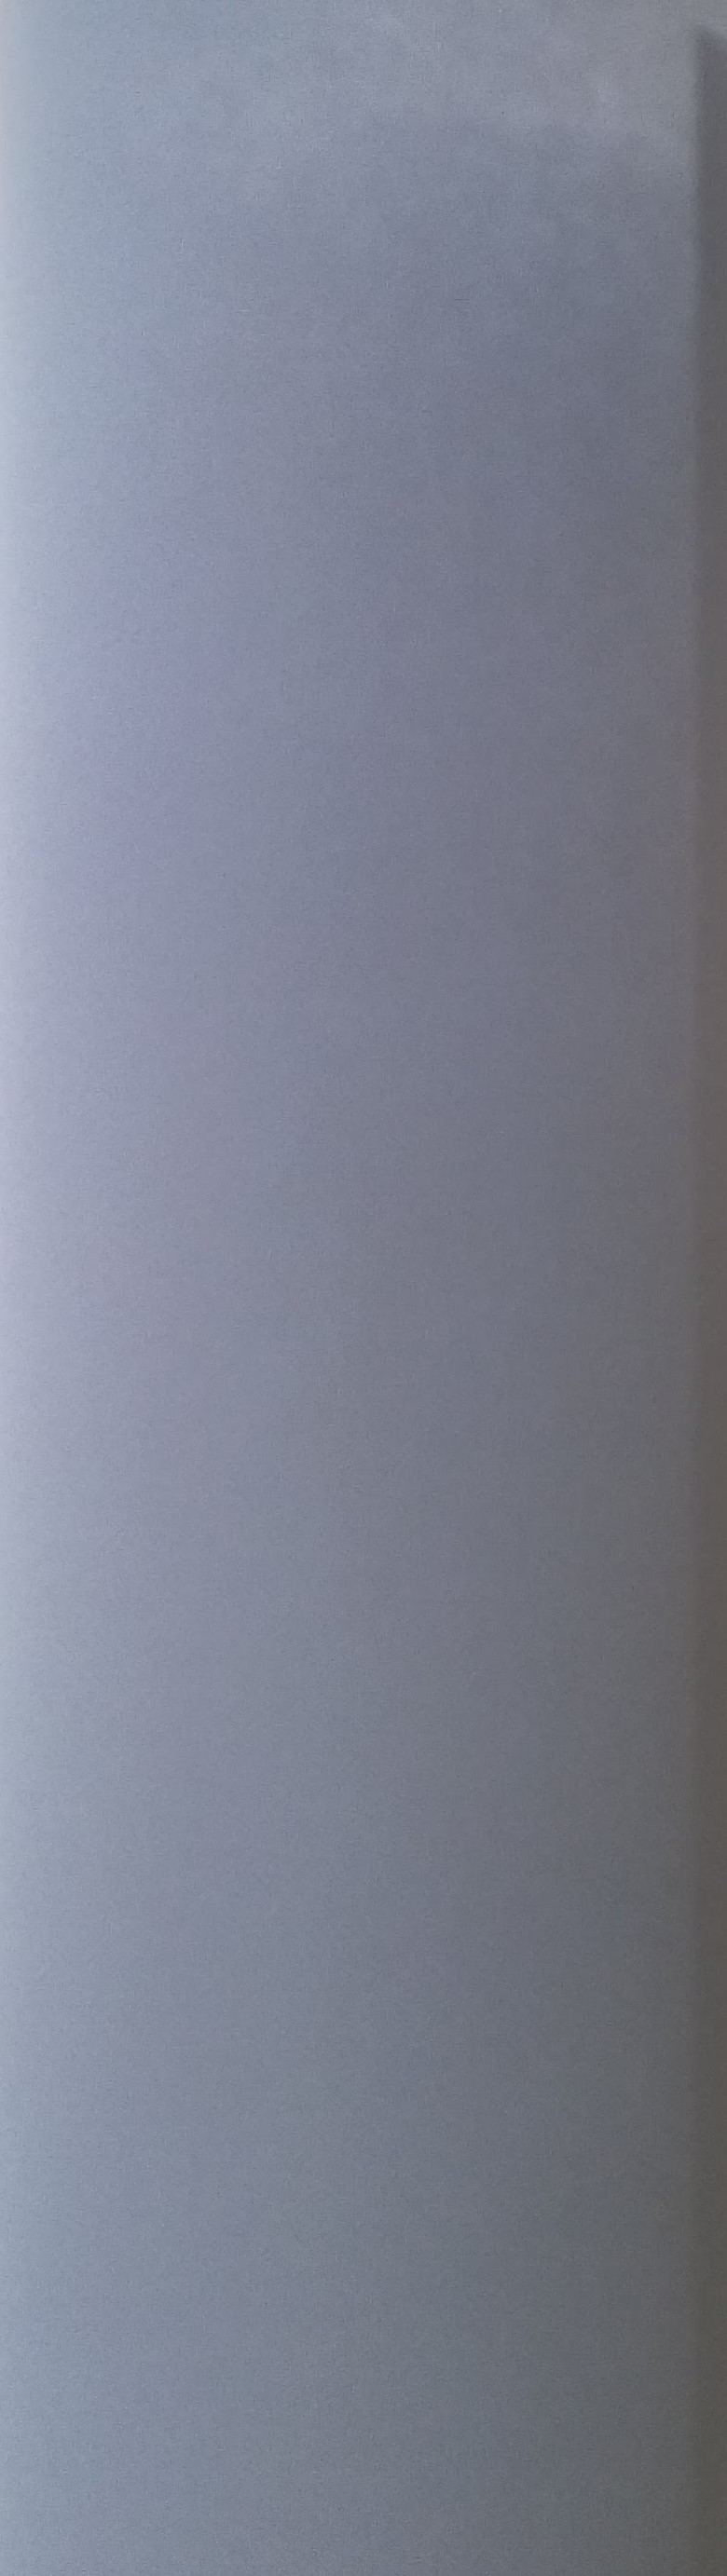
\includegraphics[width=.08\linewidth, height=.08\linewidth]{images/test_cut_02.jpg}
		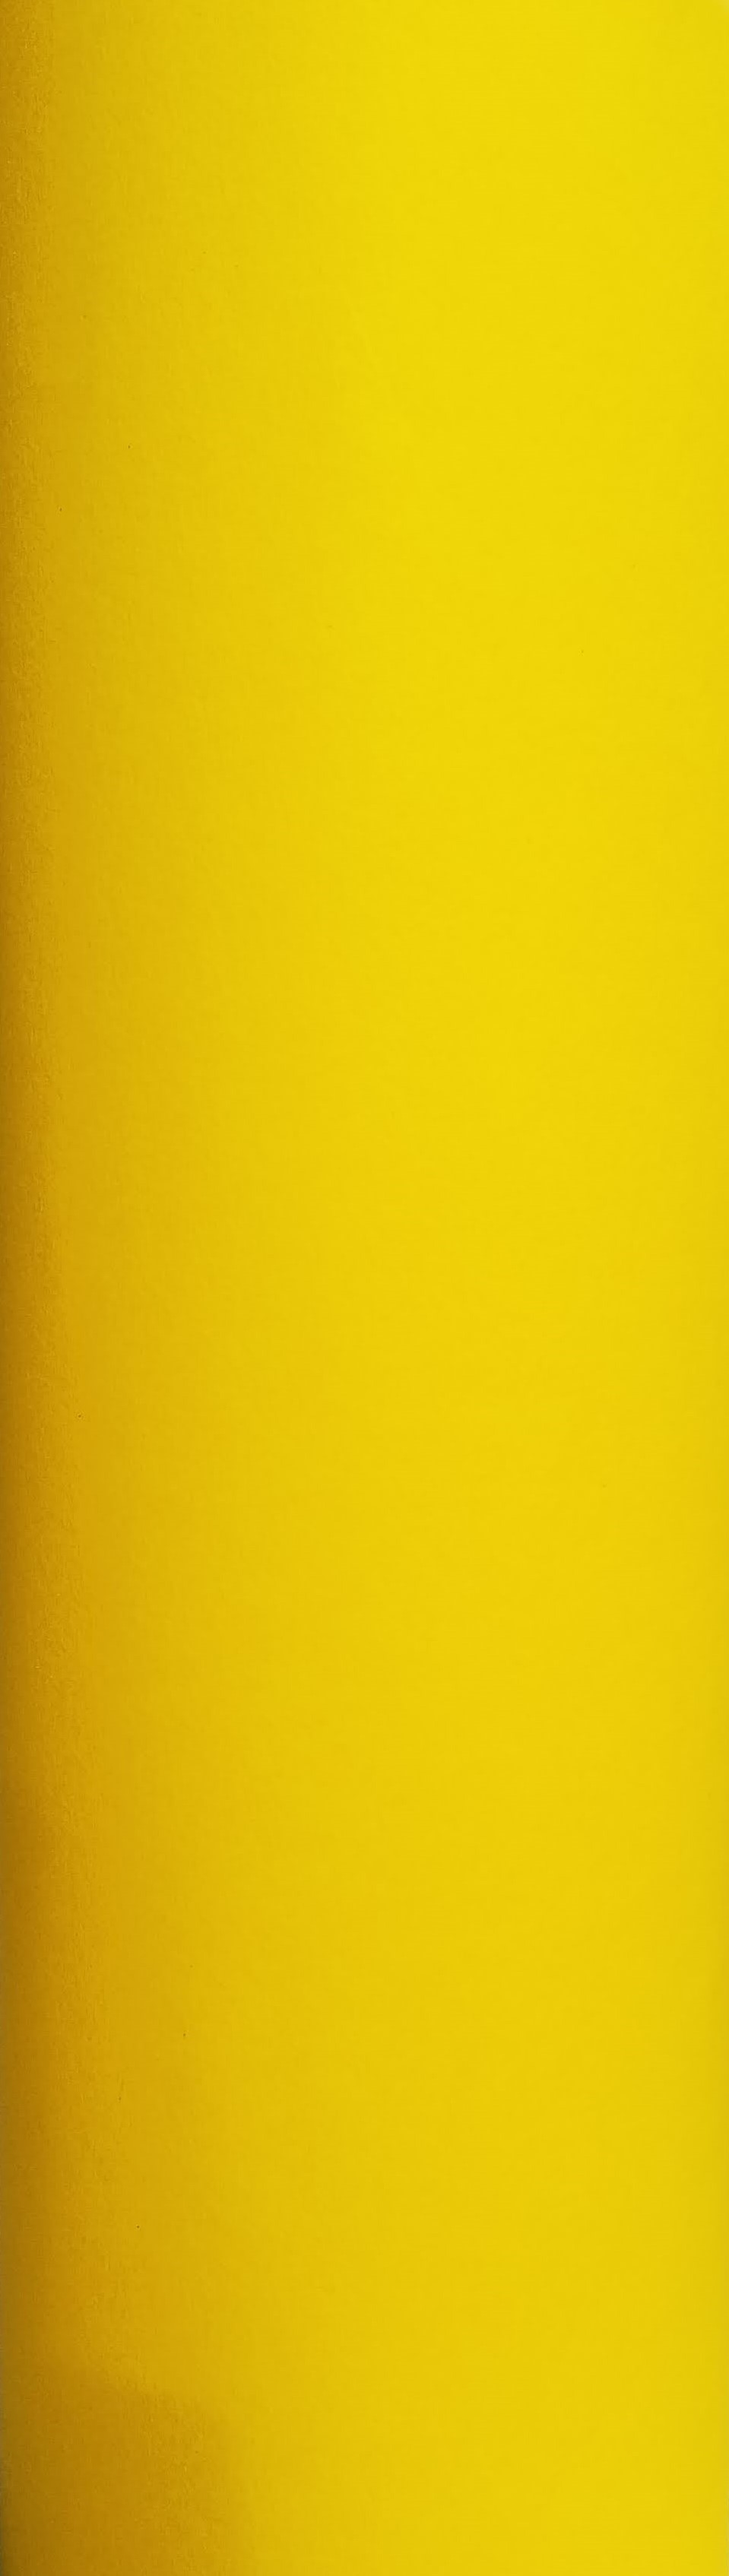
\includegraphics[width=.08\linewidth, height=.08\linewidth]{images/test_cut_03.jpg}
		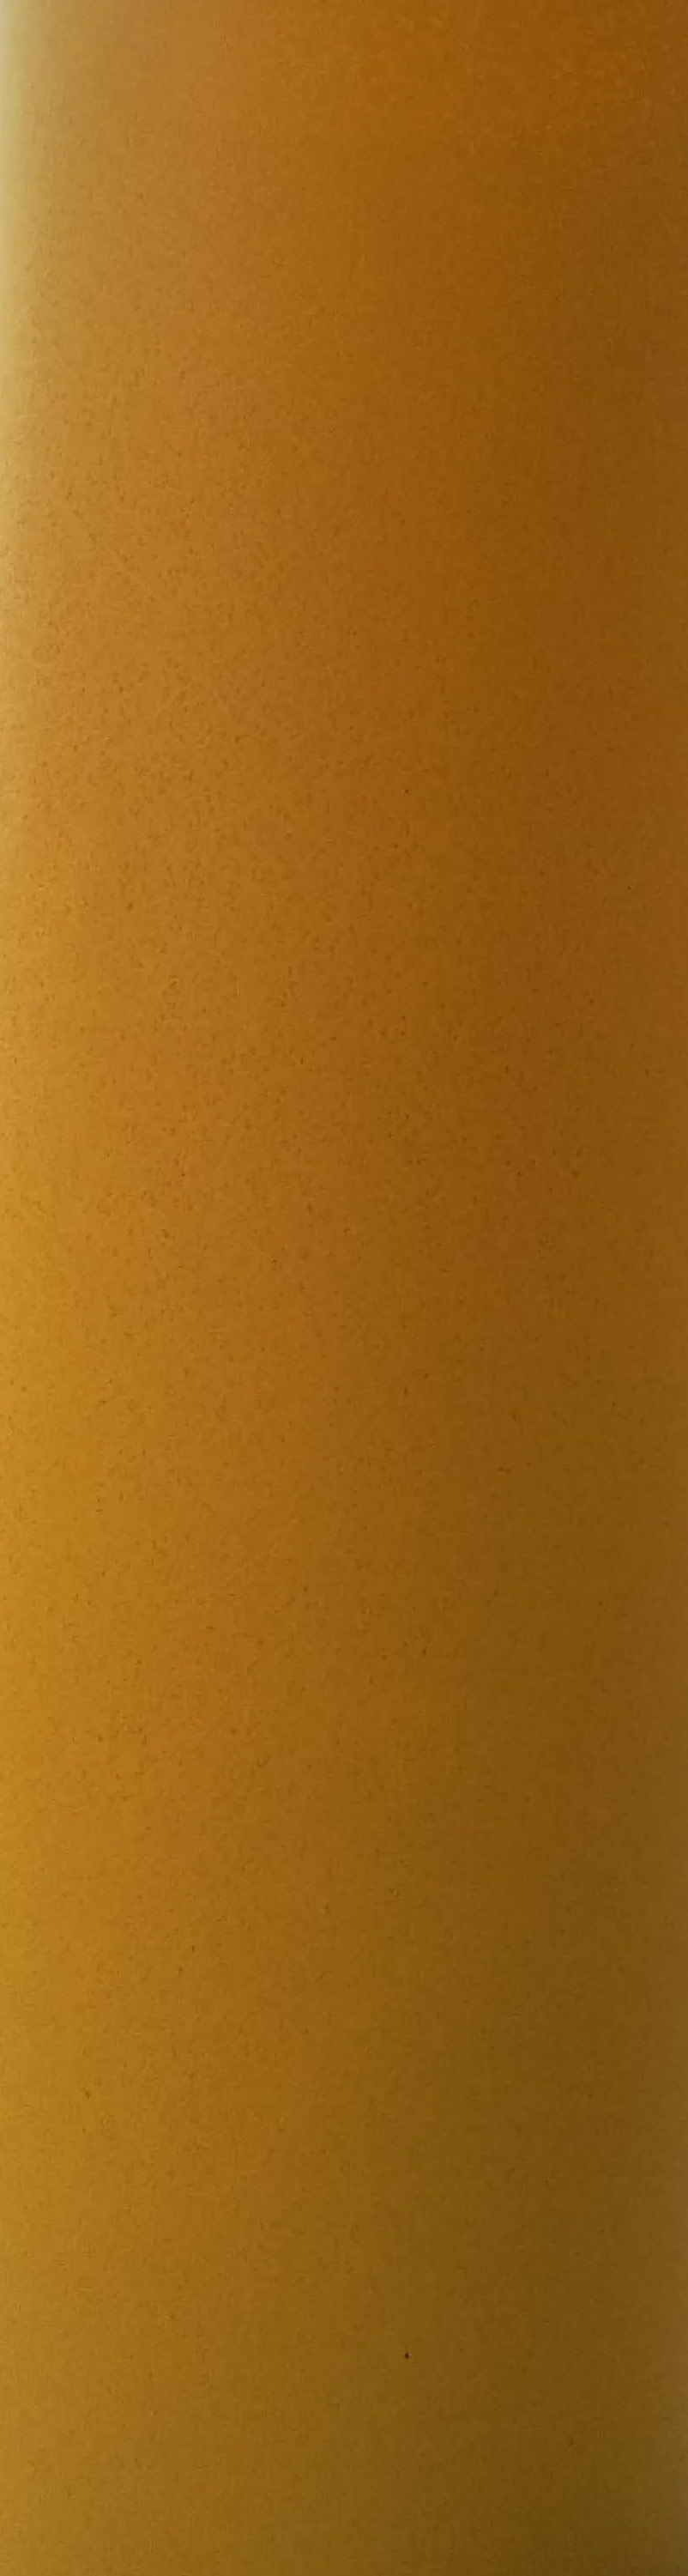
\includegraphics[width=.08\linewidth, height=.08\linewidth]{images/test_cut_04.jpg}
		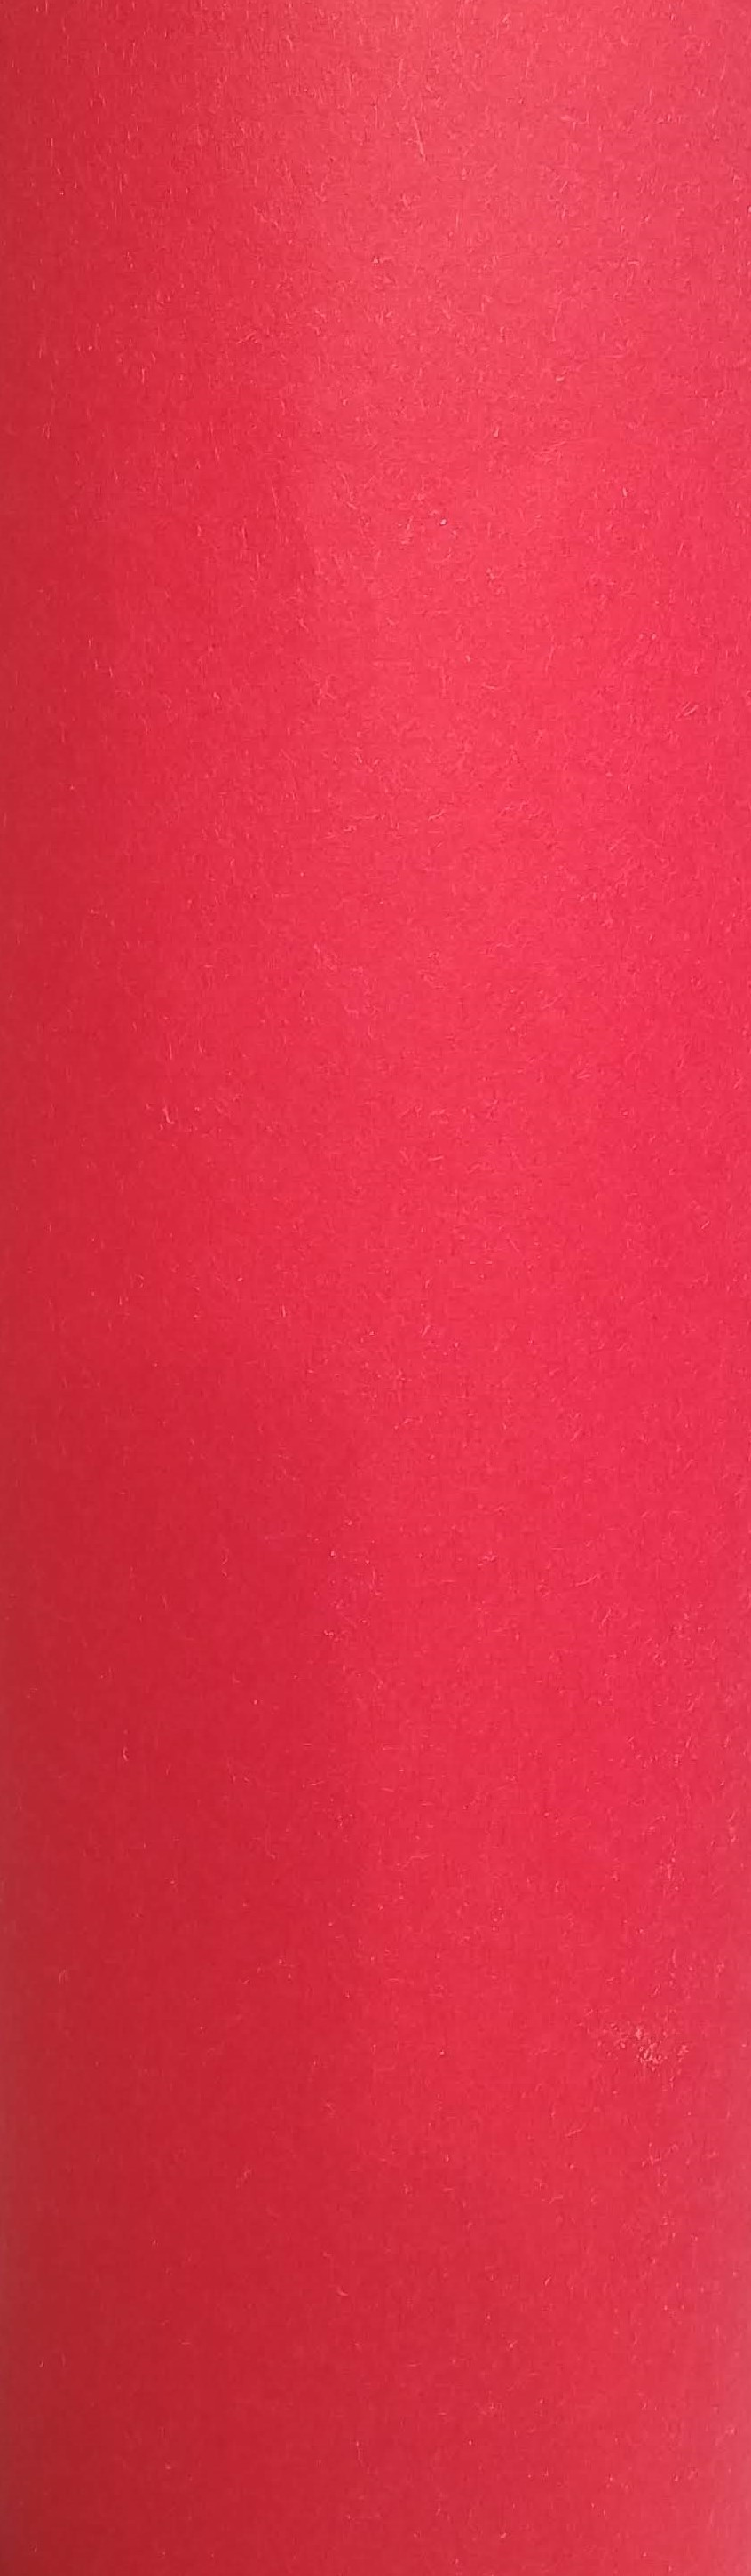
\includegraphics[width=.08\linewidth, height=.08\linewidth]{images/test_cut_05.jpg}
		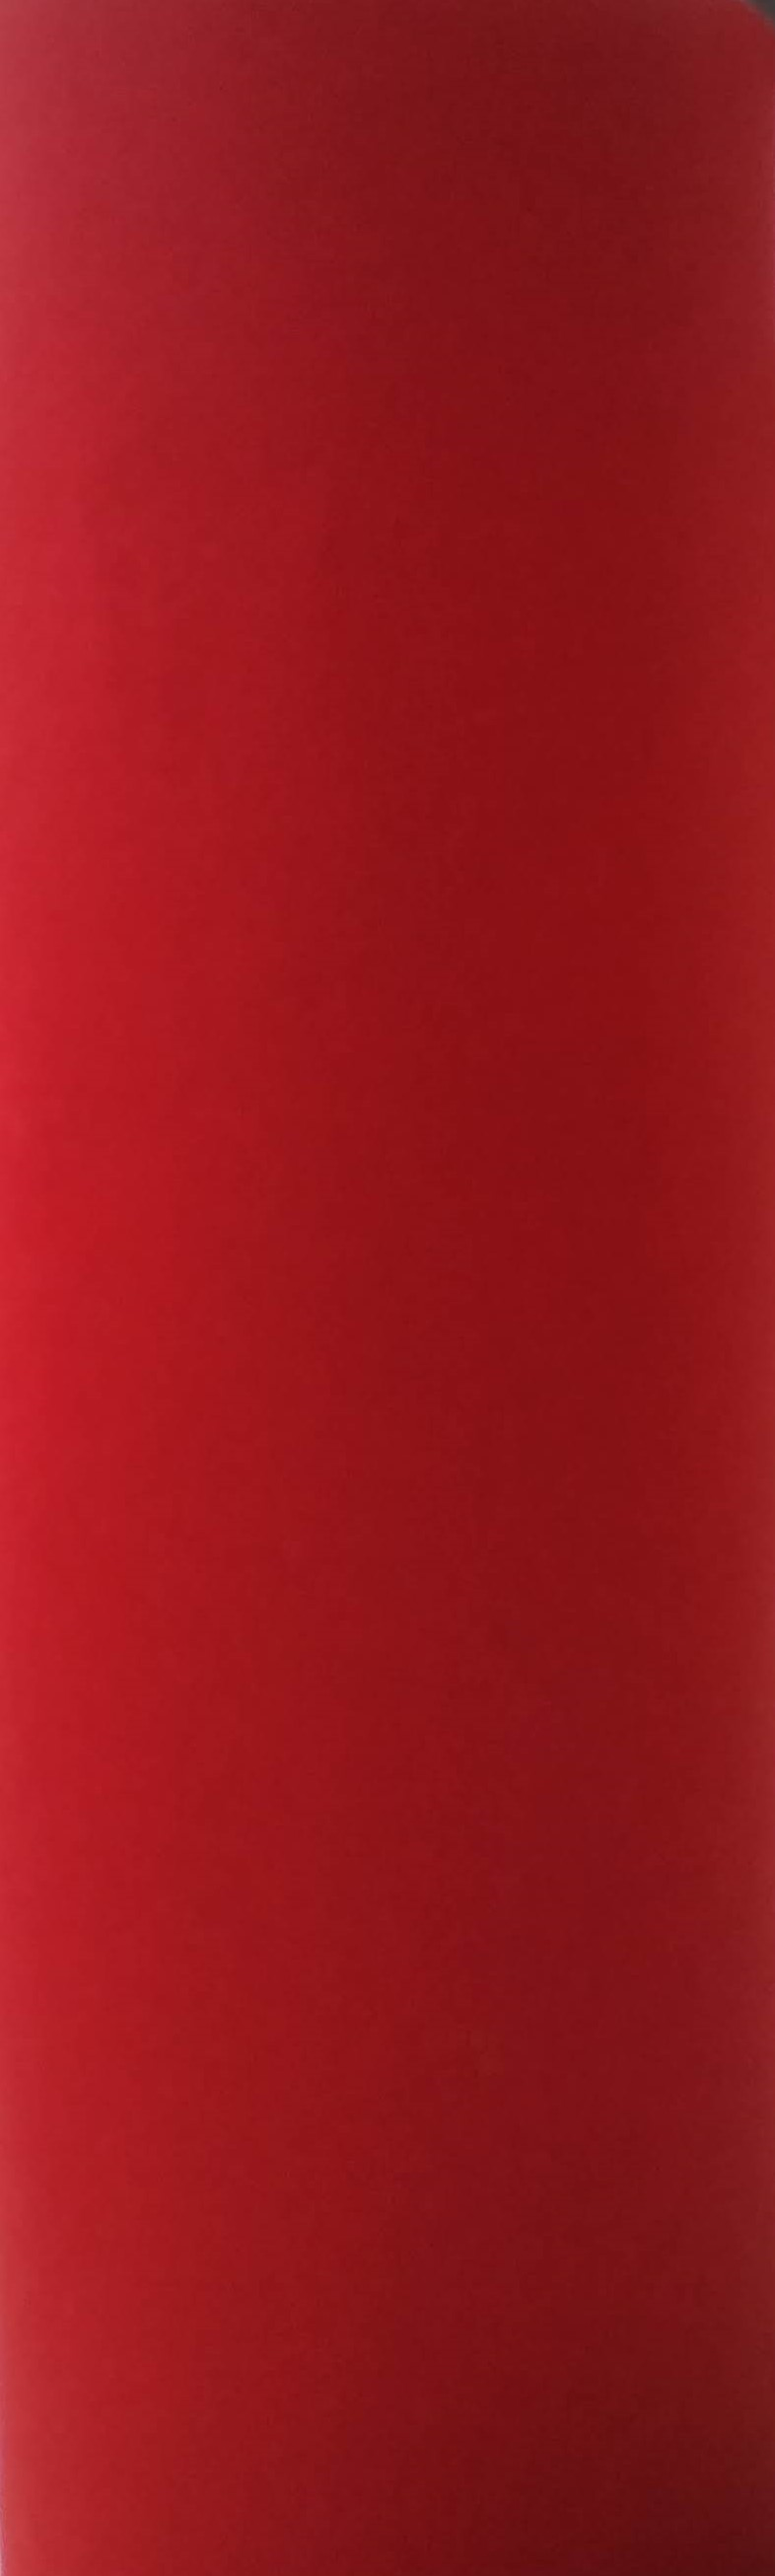
\includegraphics[width=.08\linewidth, height=.08\linewidth]{images/test_cut_06.jpg}
		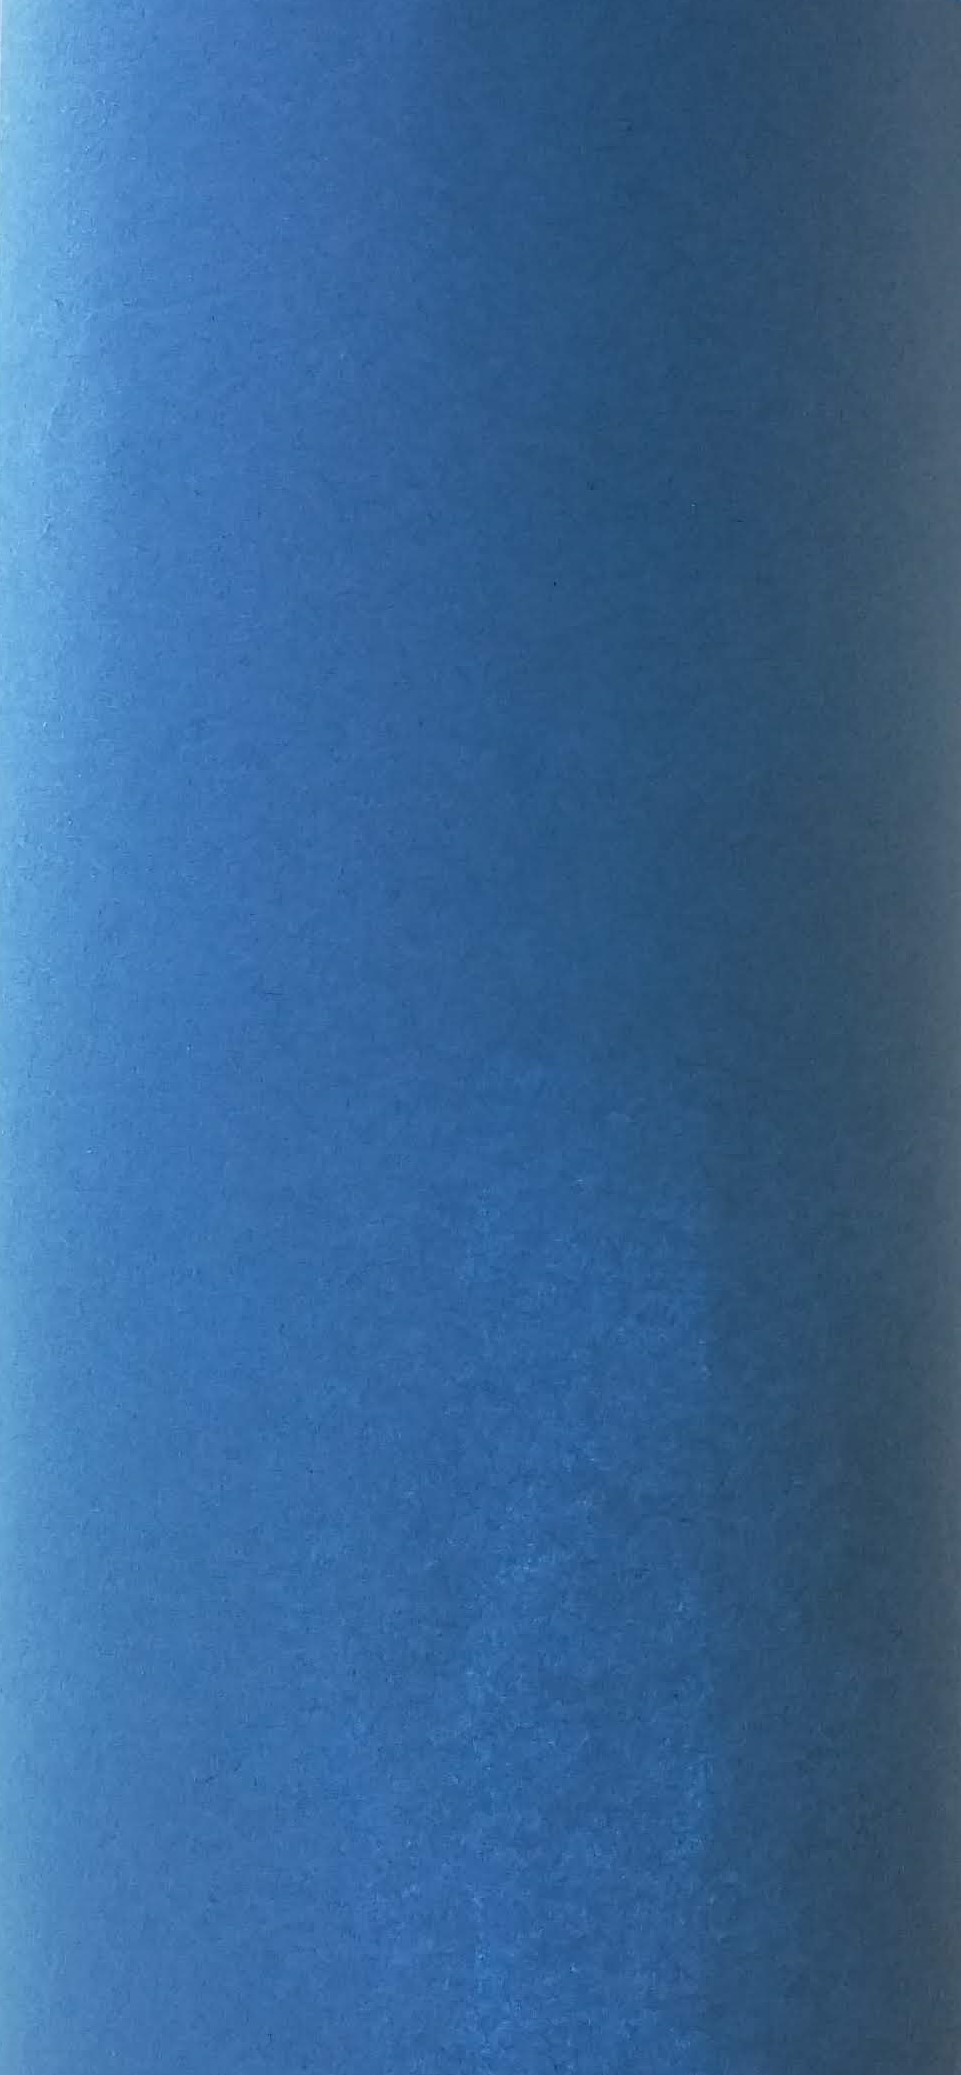
\includegraphics[width=.08\linewidth, height=.08\linewidth]{images/test_cut_07.jpg}
		
\includegraphics[width=.08\linewidth, height=.08\linewidth]{images/test_cut_08.jpg}
		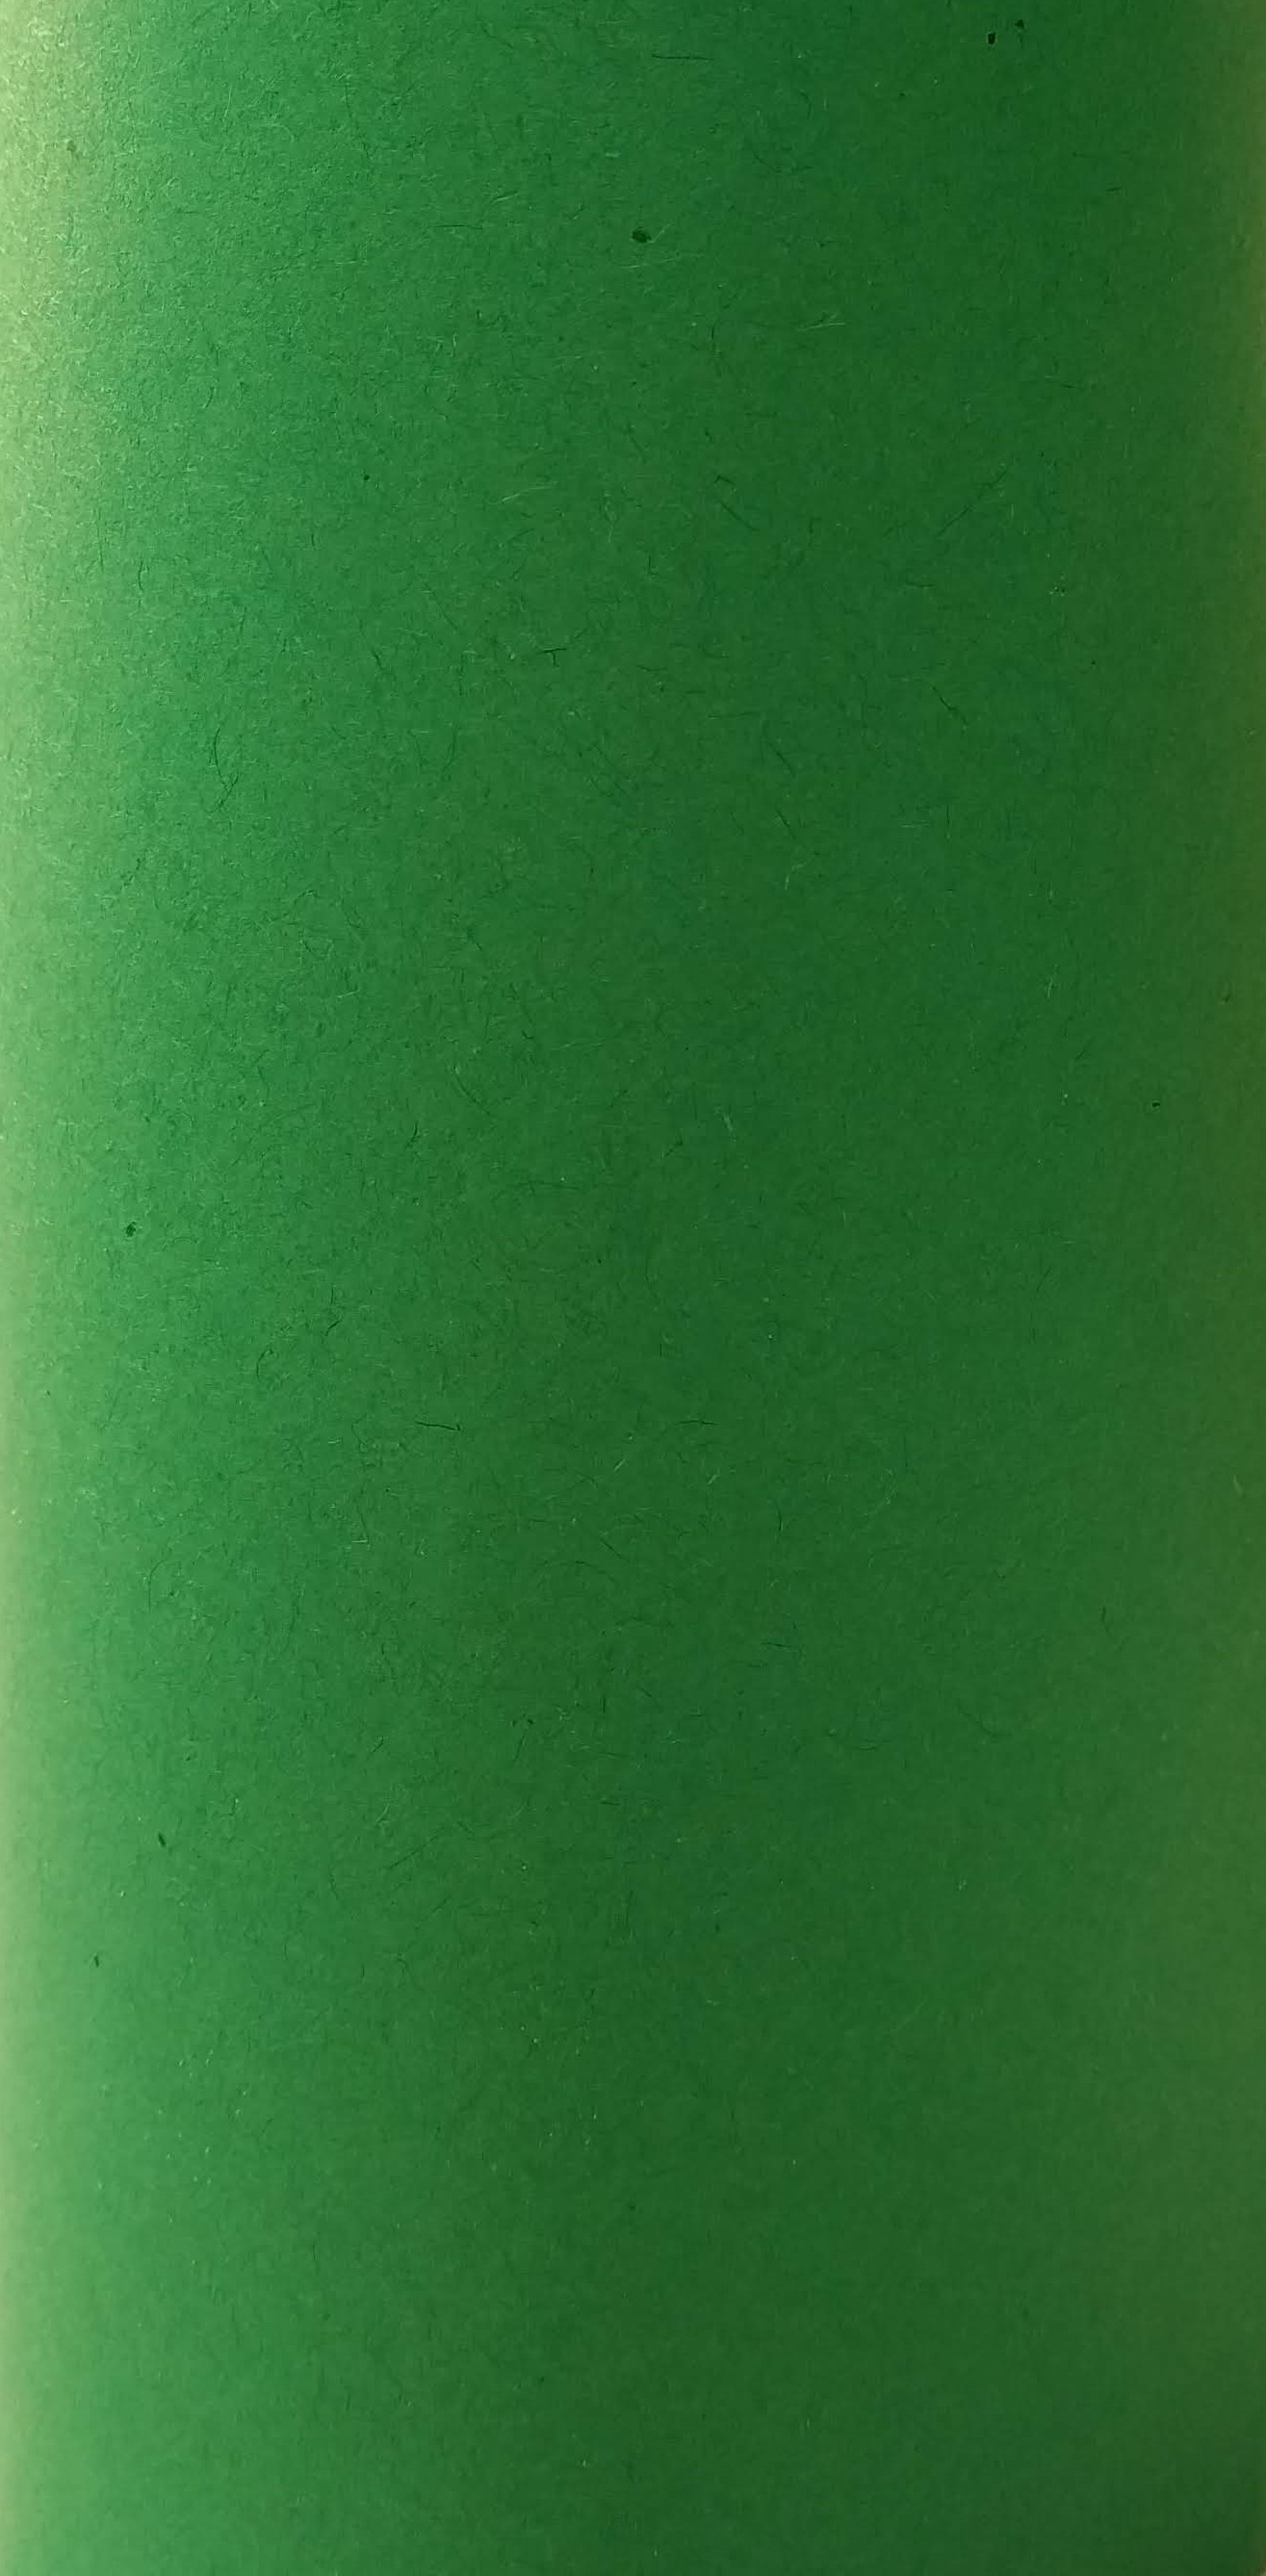
\includegraphics[width=.08\linewidth, height=.08\linewidth]{images/test_cut_09.jpg}
		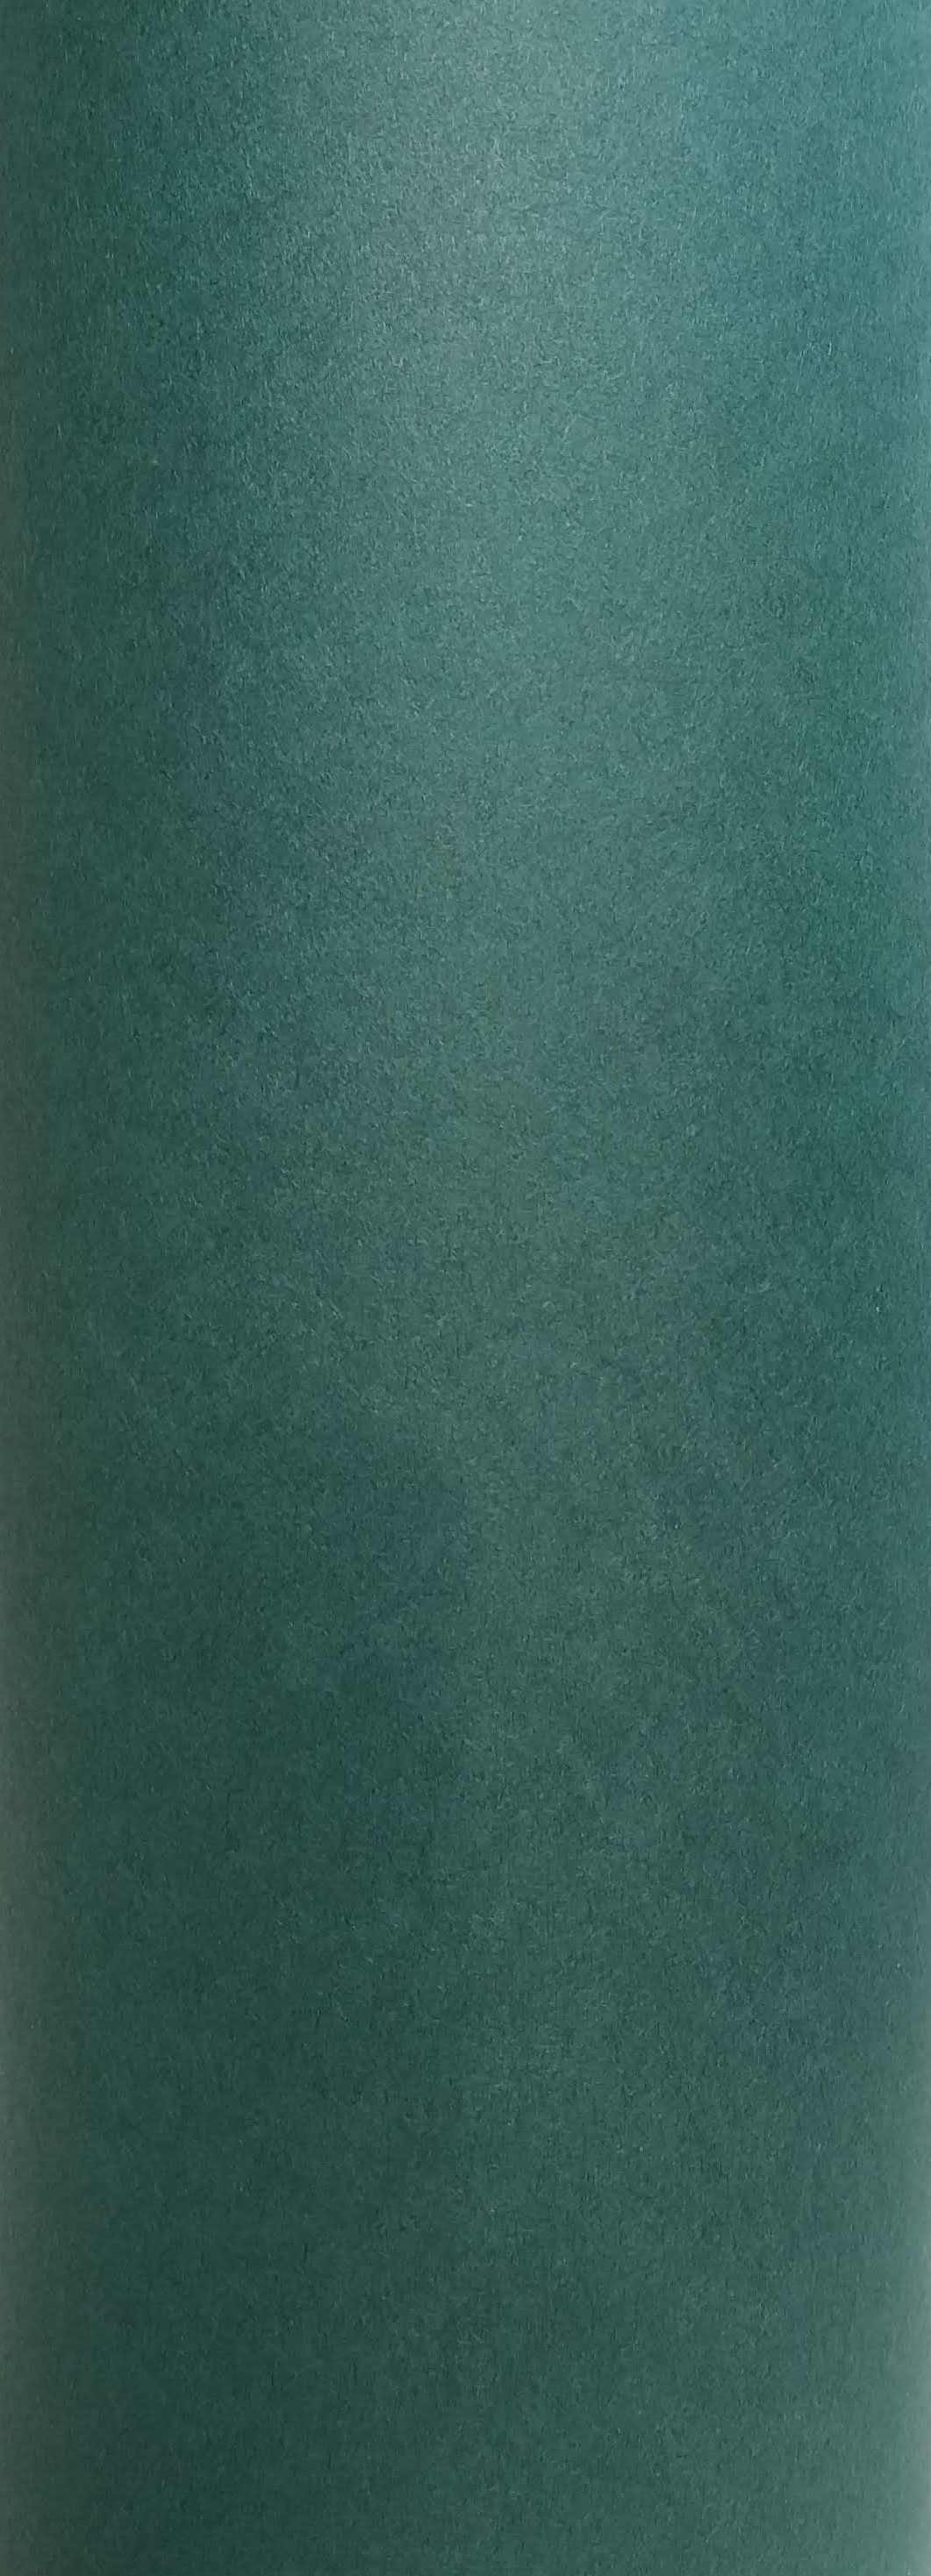
\includegraphics[width=.08\linewidth, height=.08\linewidth]{images/test_cut_10.jpg}
		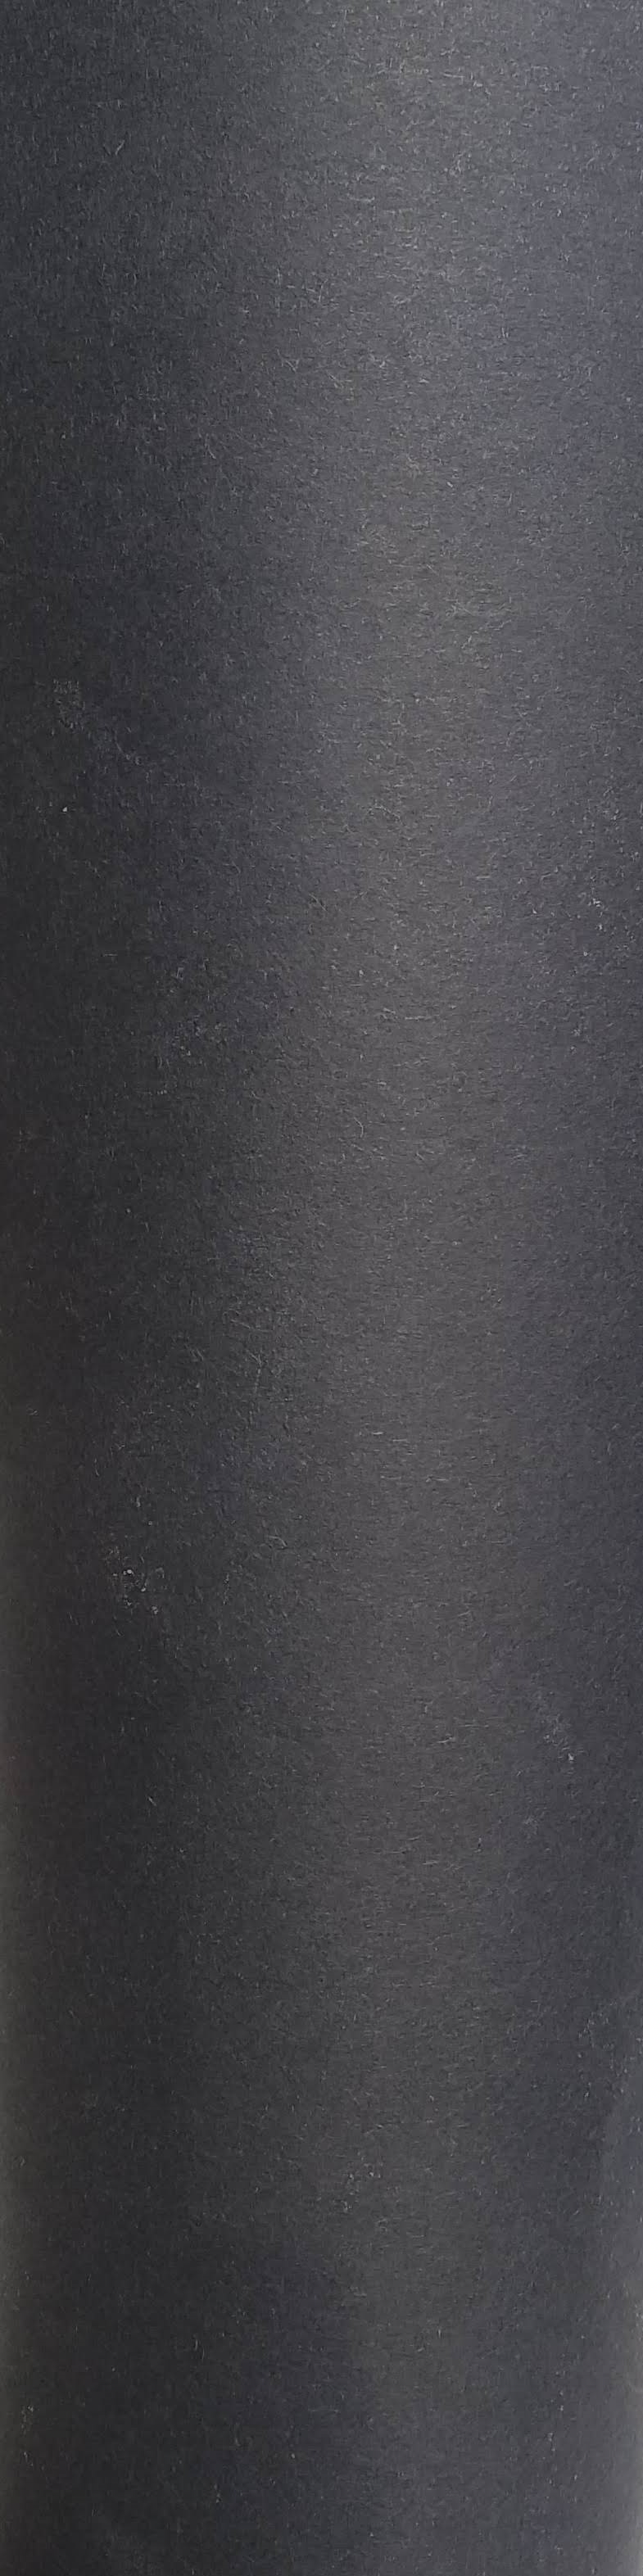
\includegraphics[width=.08\linewidth, height=.08\linewidth]{images/test_cut_11.jpg}
		\caption{Cropped images from second set}
	\end{figure}

	These cropped images illustrate very well, why we chose to use cylindrical objects as our test set. Each image contains various shades of the colour which is consequence of light hitting different spots on cylinders at different angle. Another reason for choosing this shape is that we expect encountering similar objects in the task2. 

	\subsection{Training and testing set}

	We split our data on training and testing set in a few different ways. First, we used the first set of images (circles) as our training set and the second set of images (cylinders) as our testing set. We expected this to be the best distribution, since the classifier can learn different shades of colours from the circles and then use that knowledge on images of clinders which have a few different shades of the same colour. \\

	For the second option we chose to swap the training and testing set to see if above hypotesis holds true.\\

	We noticed that the colour within each set of images is not evenly distibuted. For example, the set of images of cylinders only contains 3 photos of black cylinders as opposed to 30 photos of blue ones. We know that this might temper with the results, so we had to fix this before starting any trainig of the classifiers. \\
	
	In each image we randomly sampled the same number of points and assigned a label to each. After this was done for all images in a set, we checked which colour has the least instances and how many does it have. For each colour we then randomly selected the same number of instances as the one with the least instances have, and with this we provided equal oportunities for all colours. The process of sampling is described in more detail in the next section. \\

	Since the images of circles contain more dark tones as opposed to the images of cylinders, we expected some missclassifications.
	
	\begin{figure}[H]
		\centering
		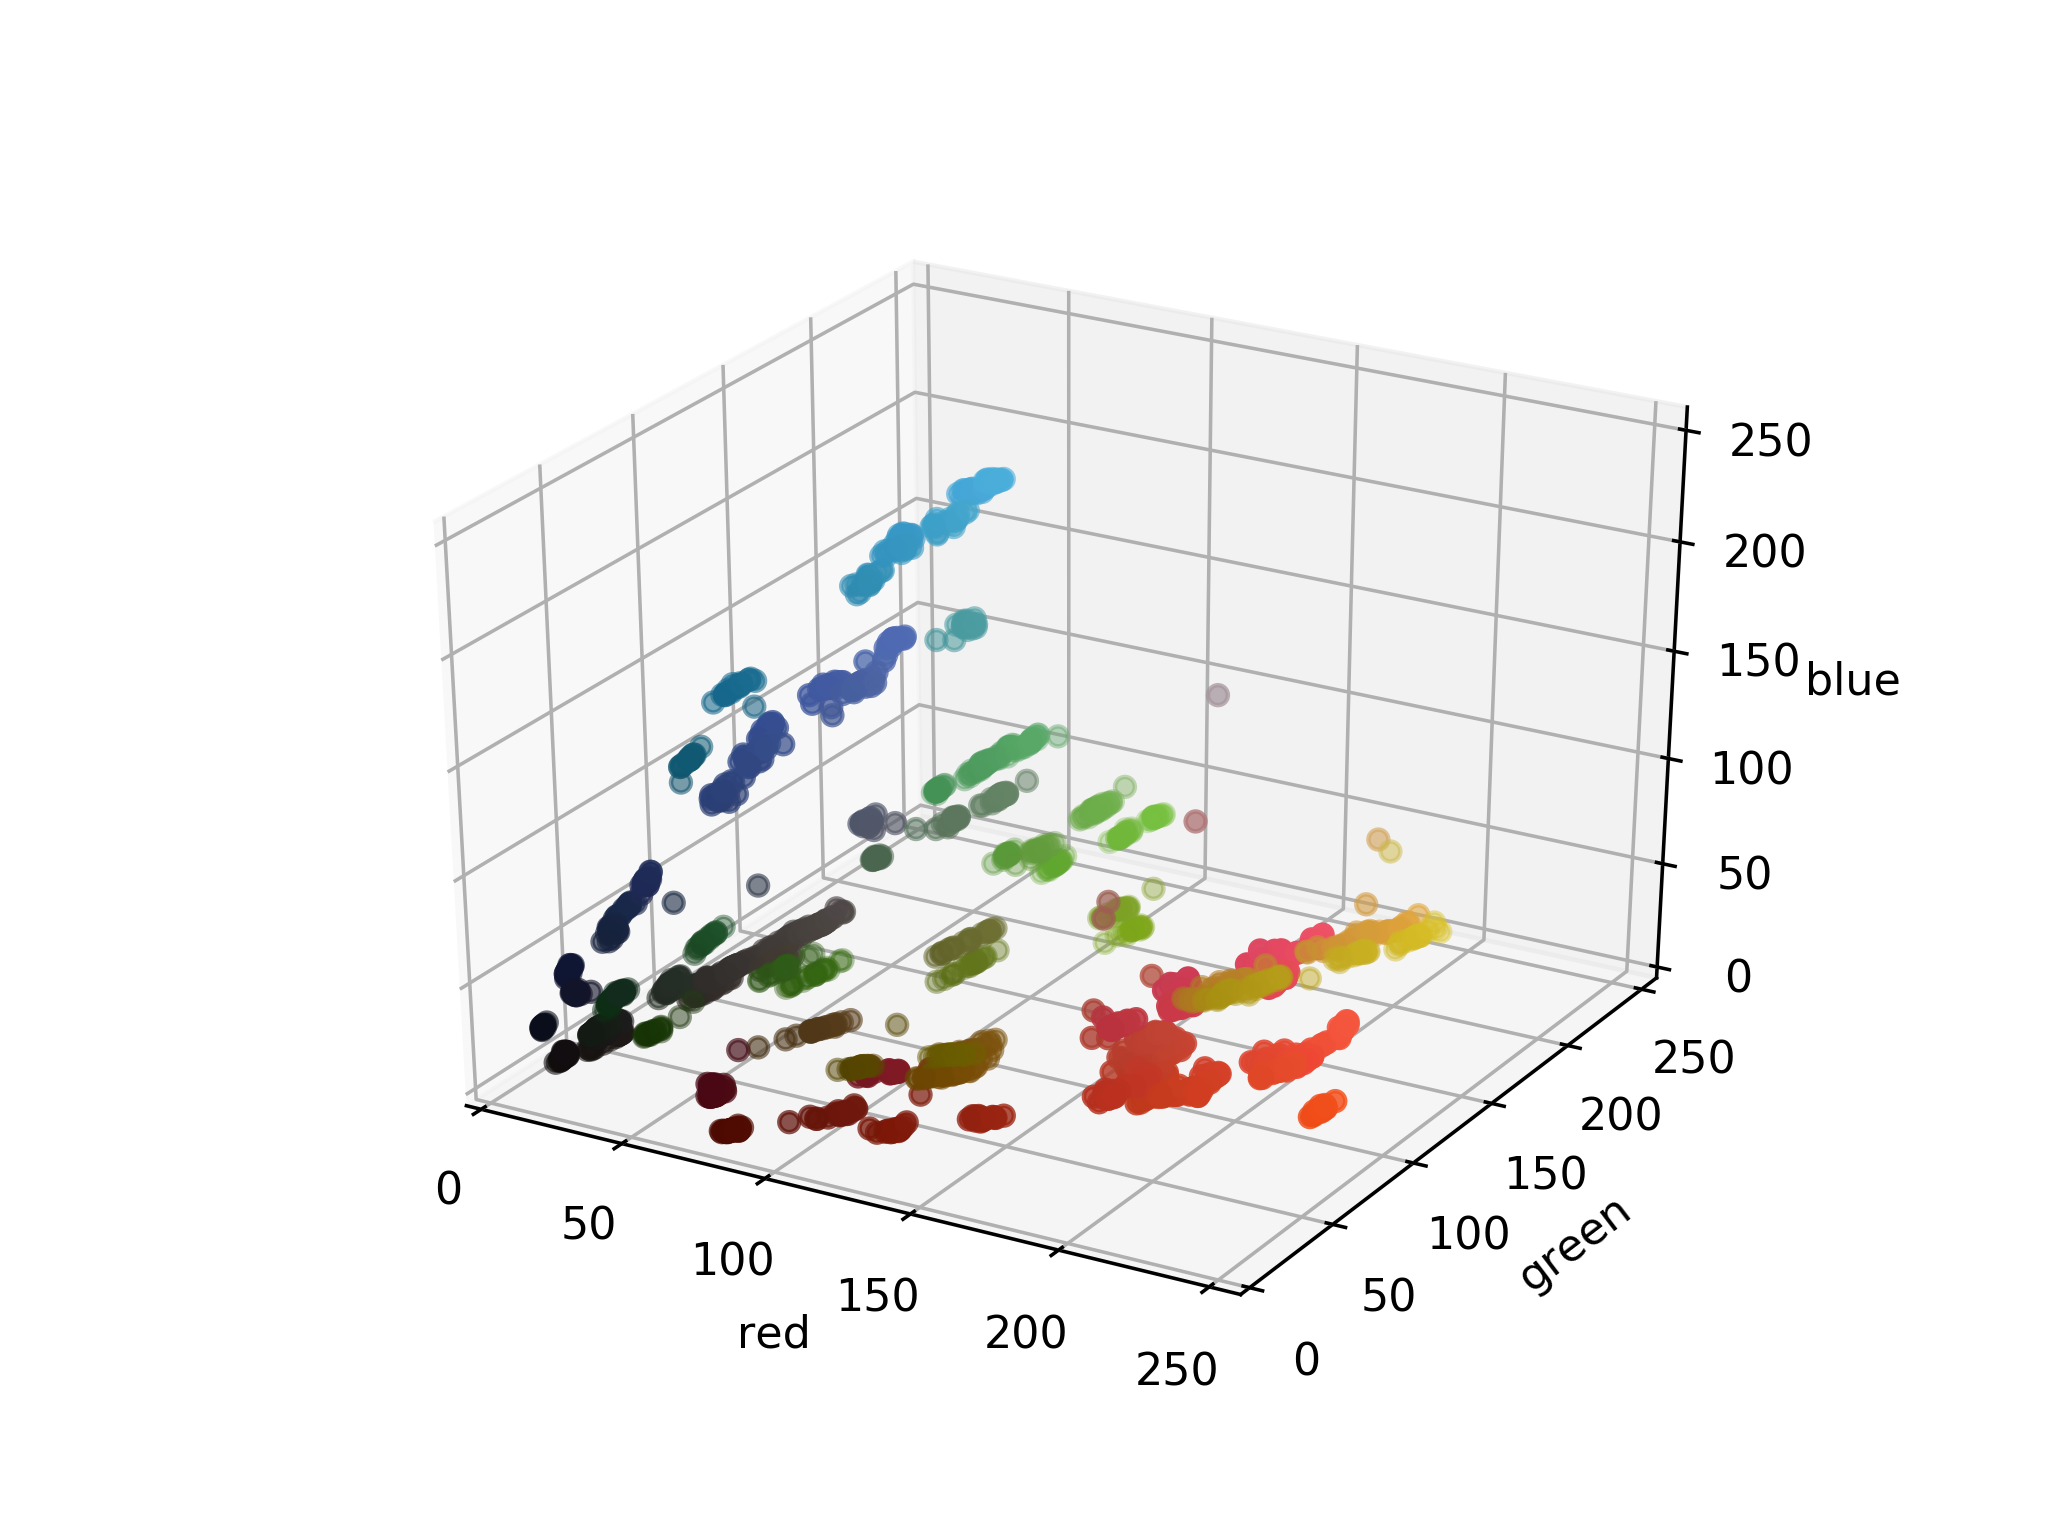
\includegraphics[width=.45\linewidth]{images/rgb.png}
		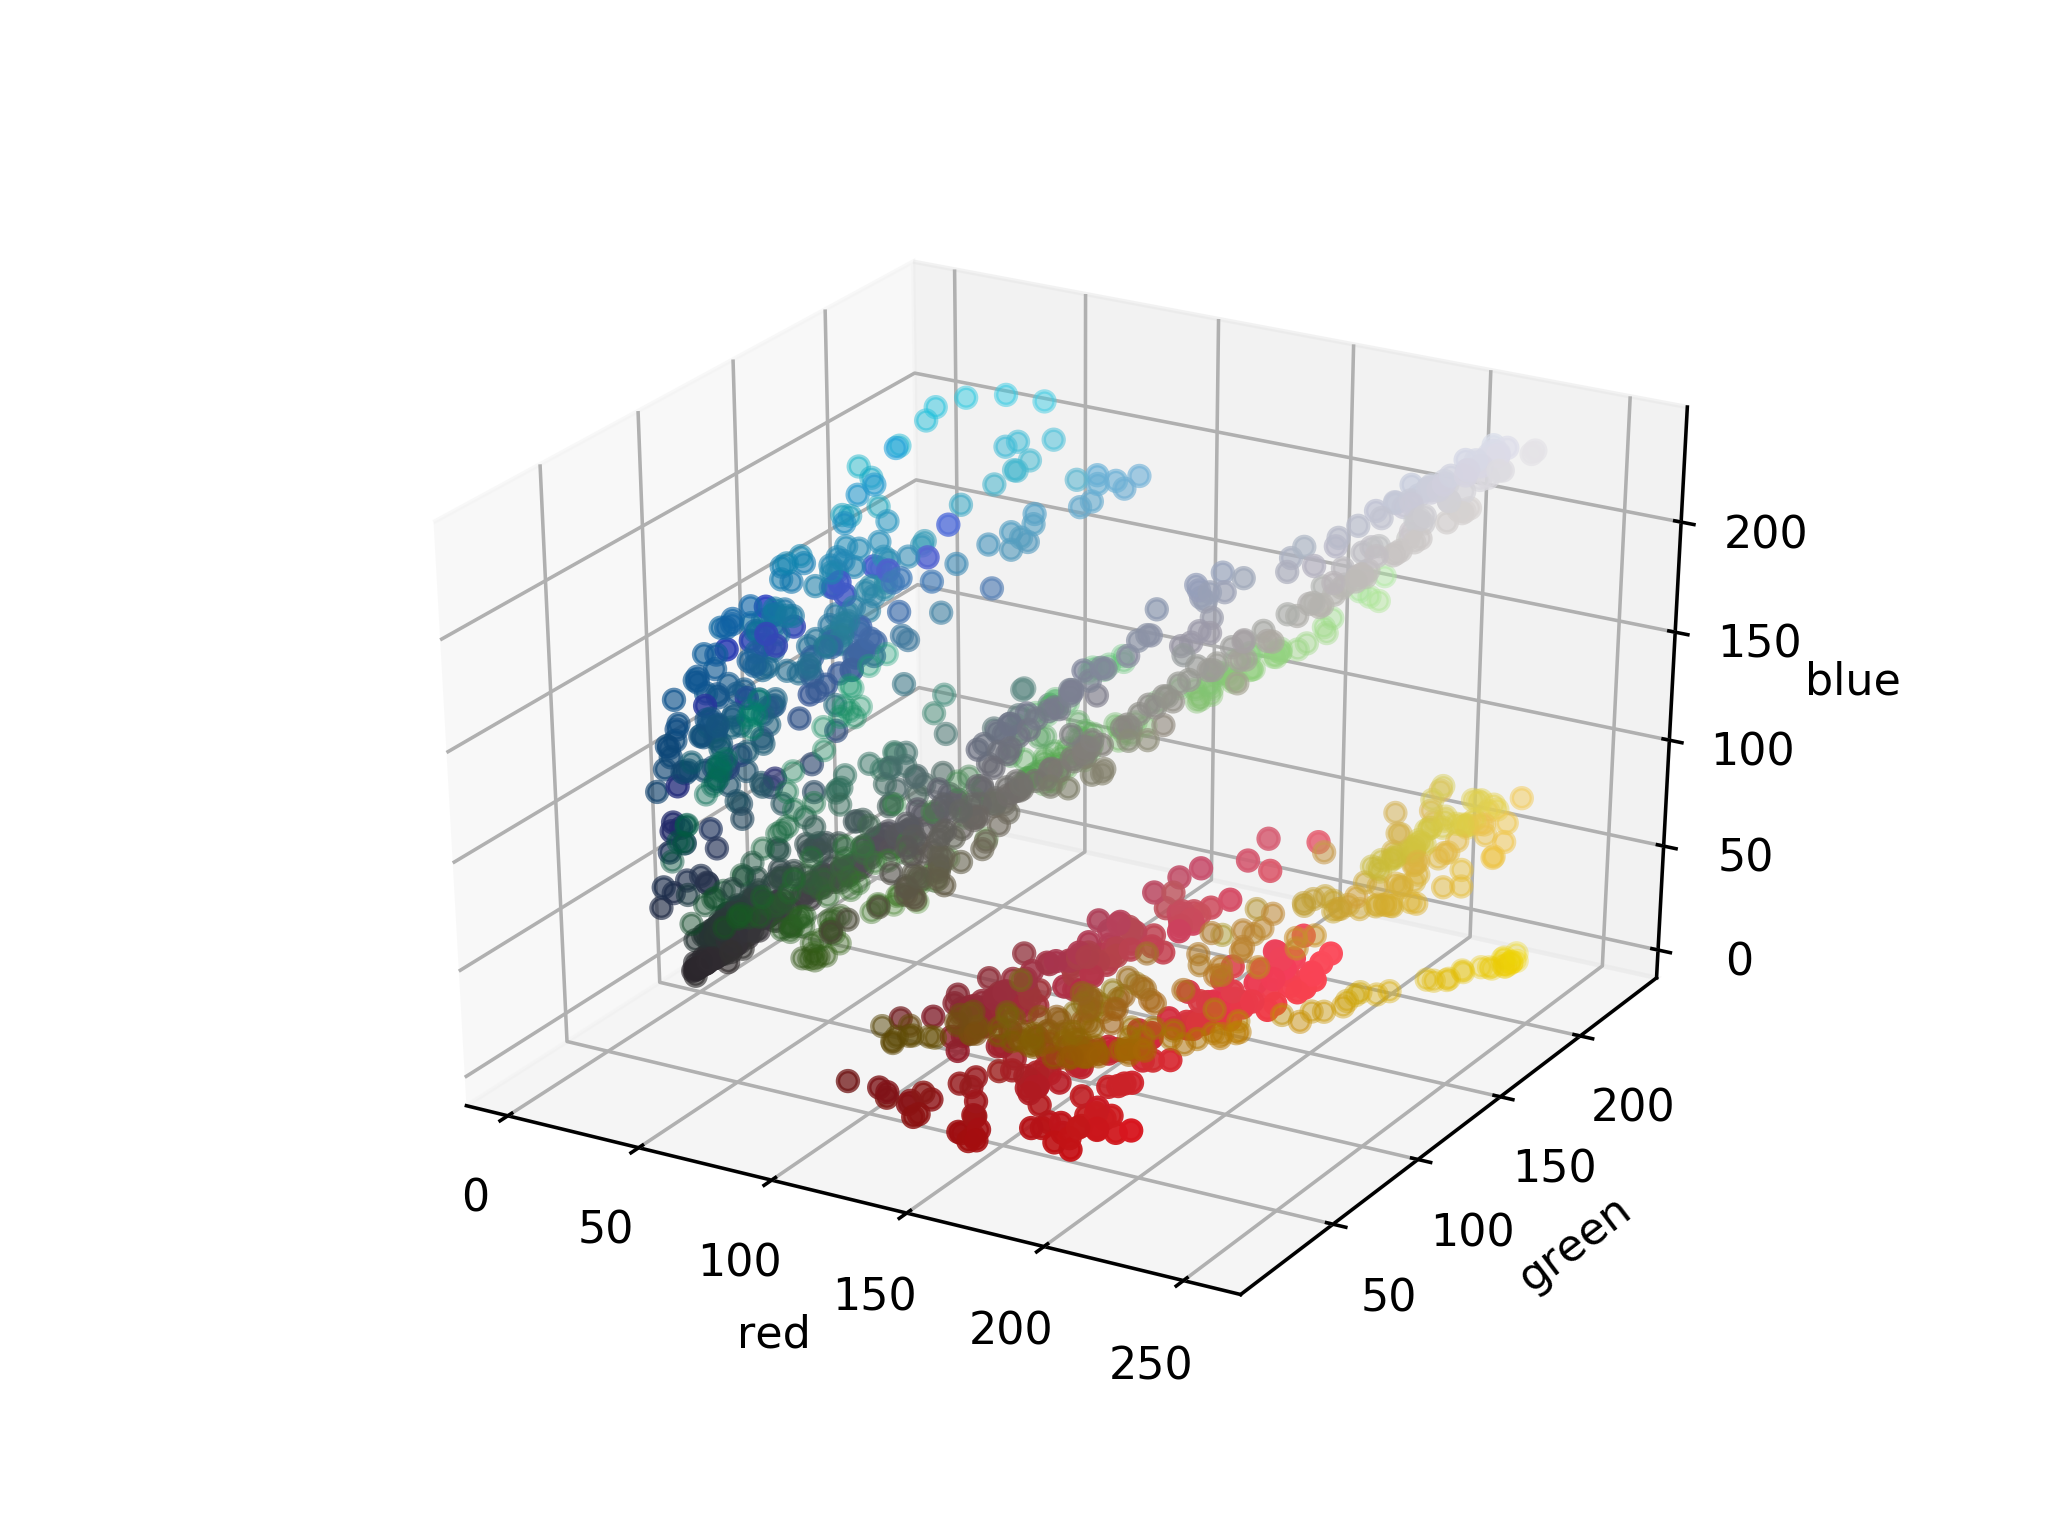
\includegraphics[width=.45\linewidth]{images/test_rgb.png}
		\caption{\texttt{RGB} colour distribution of the points in circles (on the left) and cylinders (on the right)}
	\end{figure}

	%\begin{figure}[H]
	%	\centering
	%	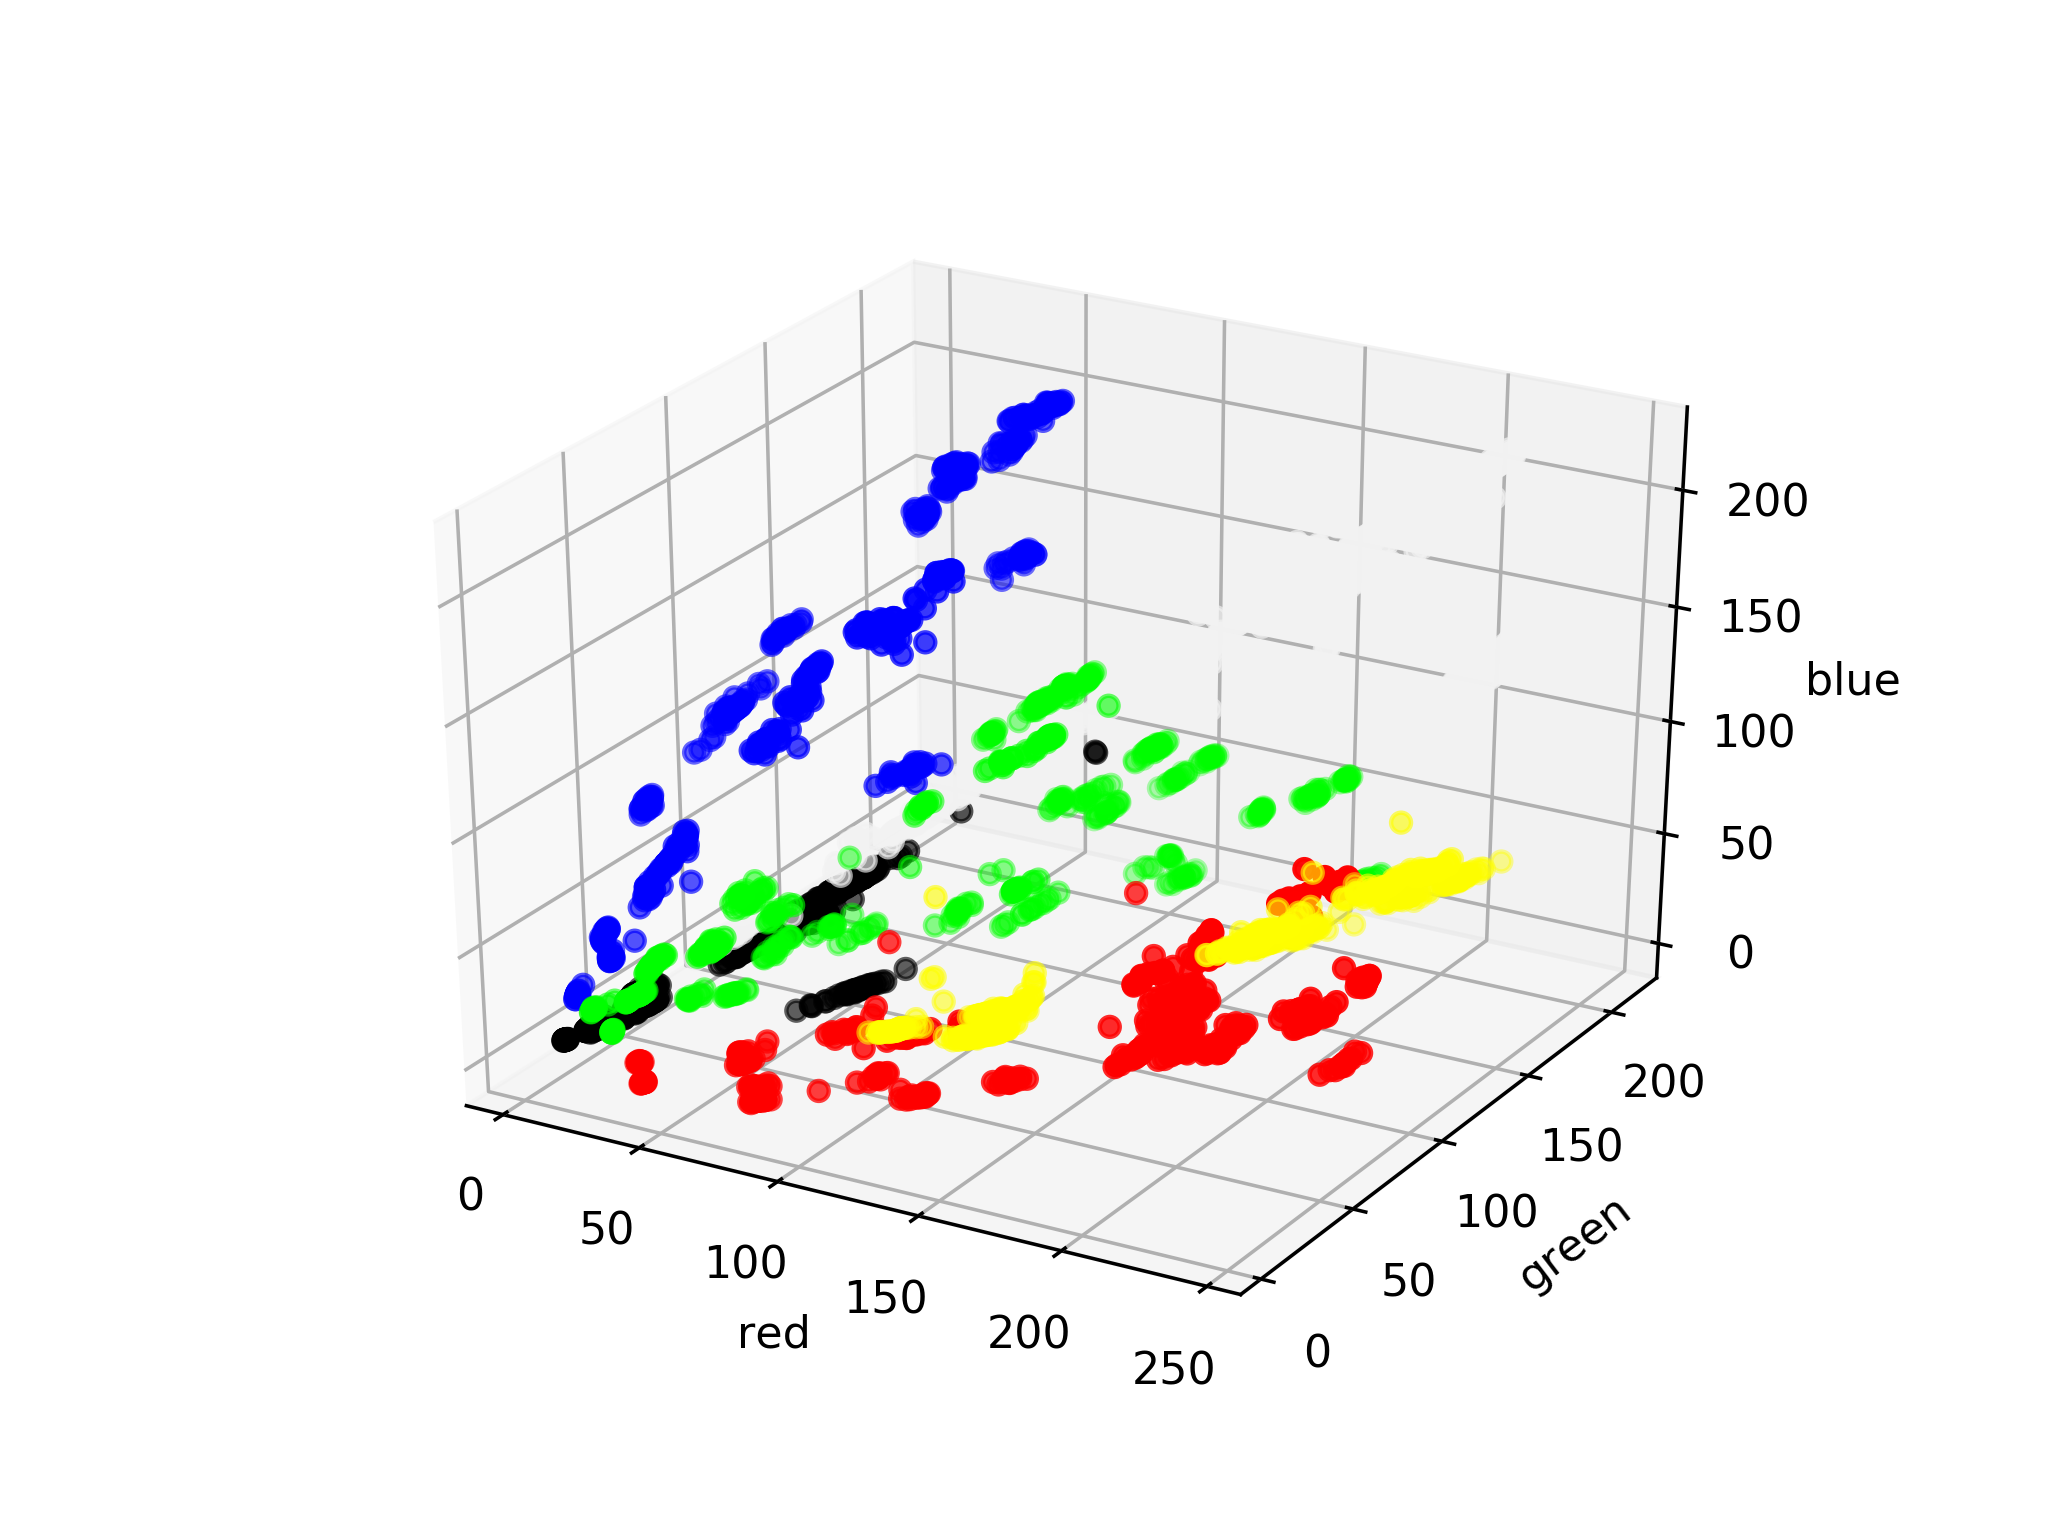
\includegraphics[width=.45\linewidth]{images/rgb_labels.png}
	%	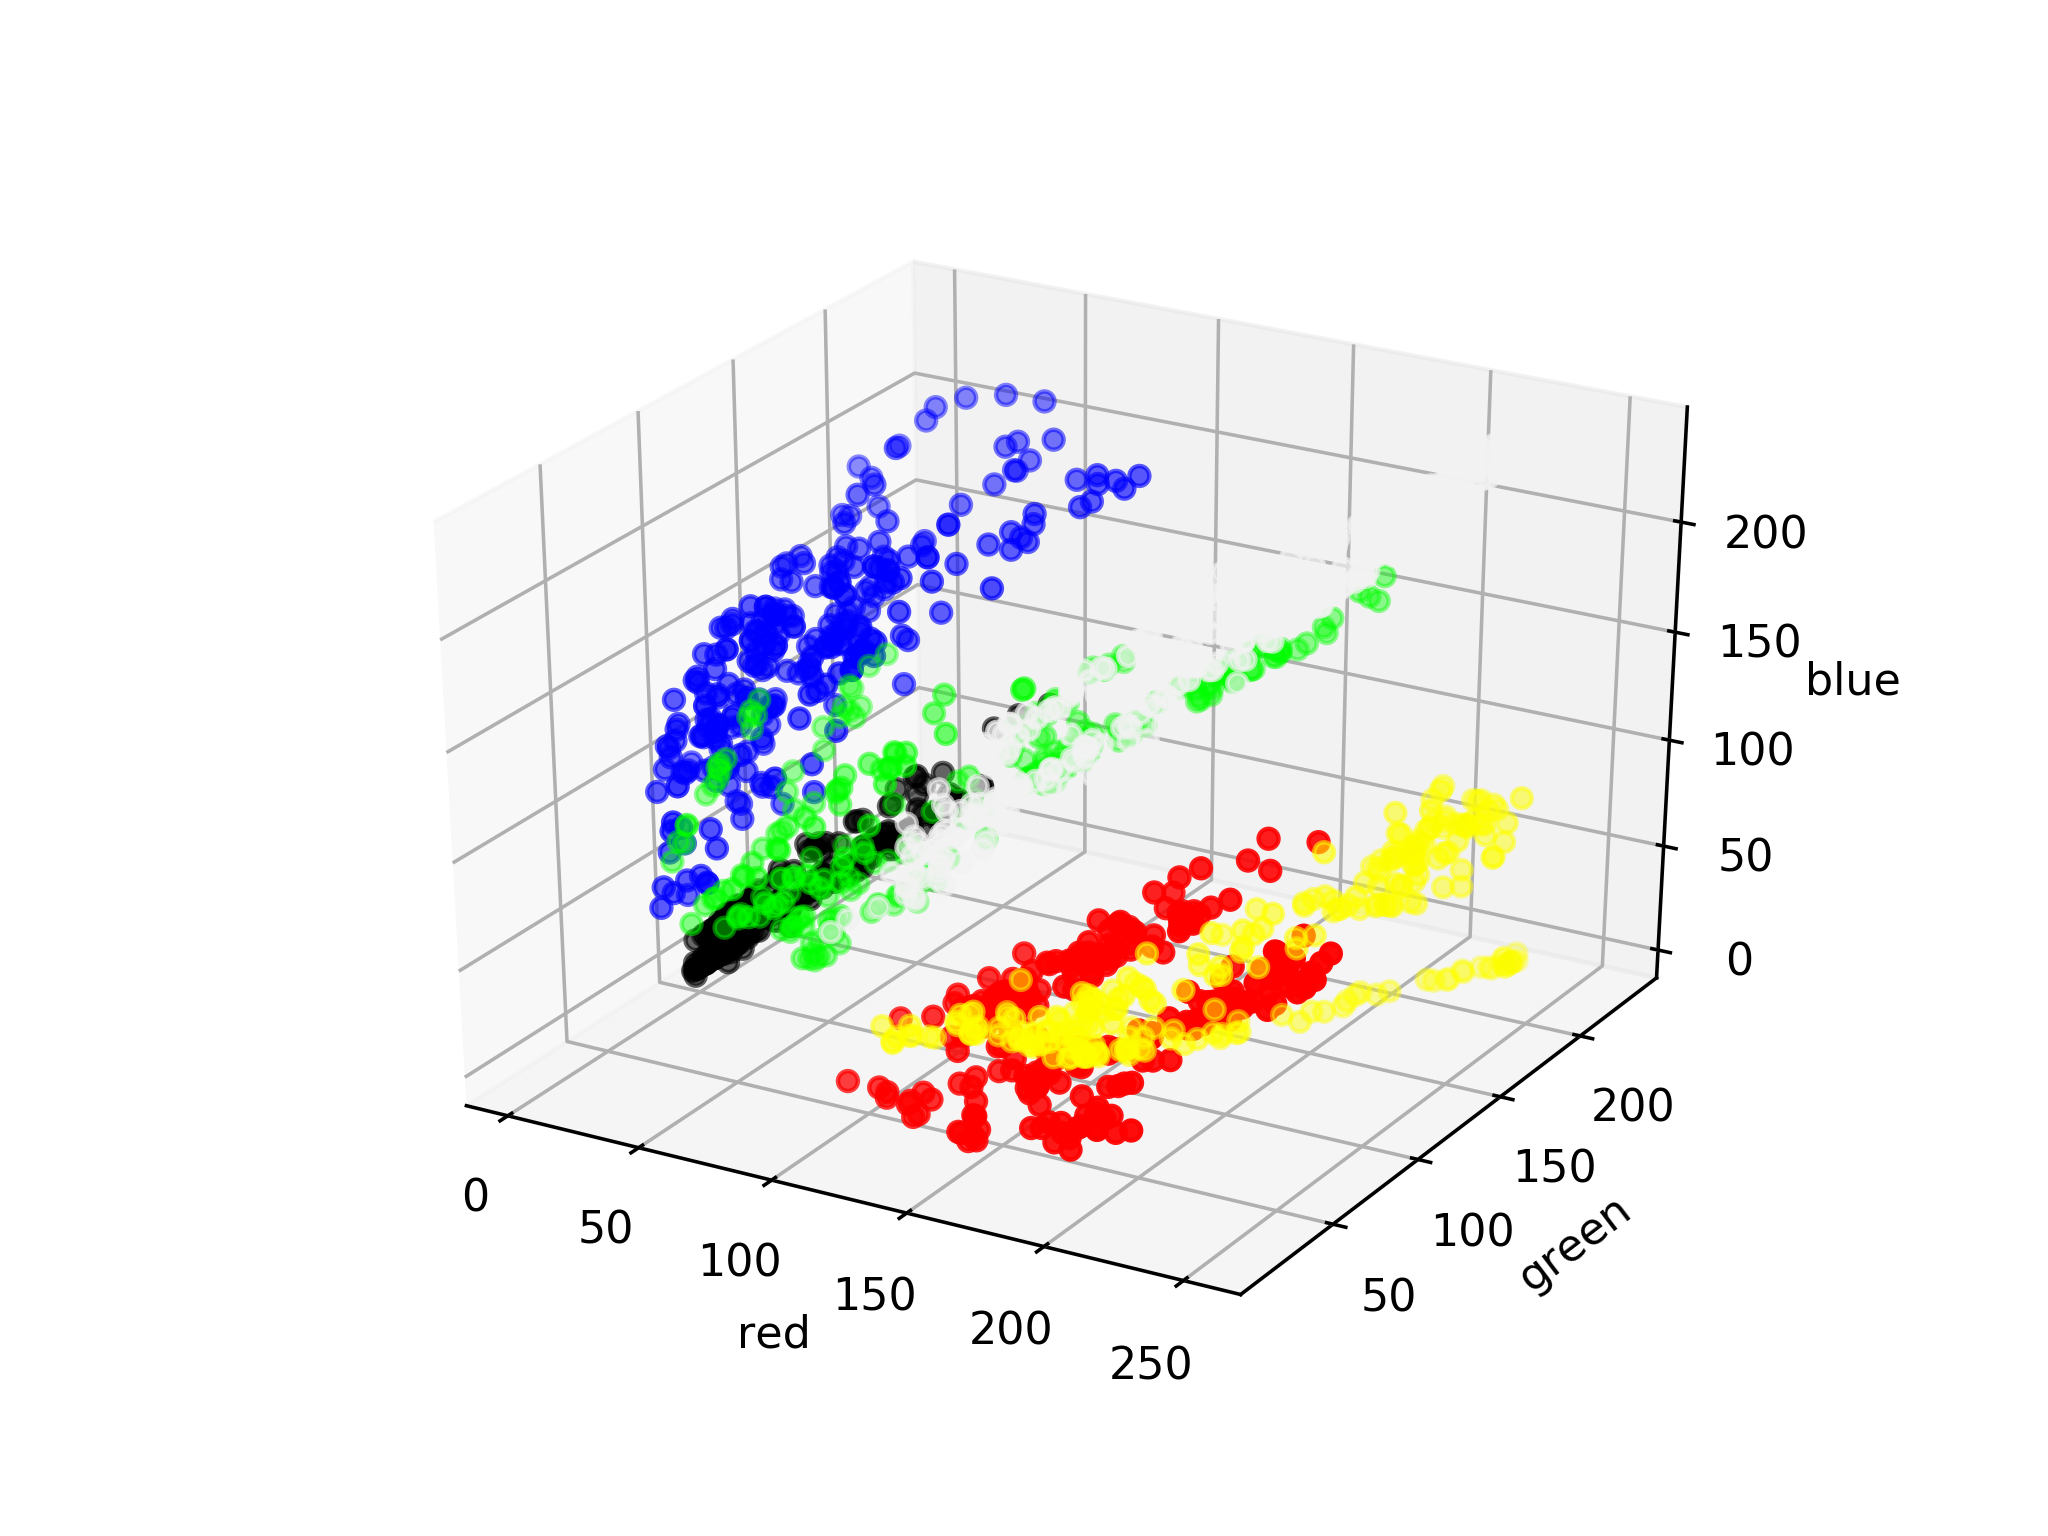
\includegraphics[width=.45\linewidth]{images/test_rgb_labels.png}
	%	\caption{Distribution of colour labels of the points in circles (on the left) and cylinders (on the right)}
	%\end{figure}
	
	\section{Colour classification}

	With our datasets ready, we then trained different classifiers to recognize colours and computed their accuracy on our testing set. To get the best classification accuracy, we also tried different colour spaces. 

	We tried \texttt{RGB}, \texttt{HSV} and \texttt{LAB} colour space.\\

	Our first approach was training a classifier with colours as input vectors. Each colour in colour space can be represented by a vector $v$ and the classification task is to map this vector $v$ to correct class. \\
	
	In the \texttt{RGB} colour space, each vector $v$ can be represented using $v = (red, green, blue)$, where $red, green, blue \in [0, 255]$. \\

	Because the input to our classifier is a simple three dimensional vector, we predict that the knn classifier will perform quite well. \\	
	
	To prepare training data set, we used Hough transformation to detect circles in our images and randomly sampled points inside found circles to obtain \texttt{RGB} vectors corresponding to colours. Instead of sampling colour just from one point in the circle, we averaged colours in a region around sampled point. We chose multiple points from the same circle because object's illumination is almost never uniform. \\
	
	In the figure below we have plotted colours from our first training set (circles) in \texttt{RGB}, \texttt{HSV} and \texttt{LAB} colour space. As we can see, in the \texttt{RGB} colour space, the shades of the same colour lie on the same line. Similar thing happens in \texttt{HSV} colour space, but the lines are vertical. Because the \texttt{HSV} colour space is conical, the red colour lies both on the far left and far right of our graph. This is not ideal for knn or linear support vector machines, so we predict that those will perform better on the \texttt{RGB} colour space. \\

	\begin{center}
		\begin{figure}[H]
			\begin{subfigure}{.5\linewidth}
				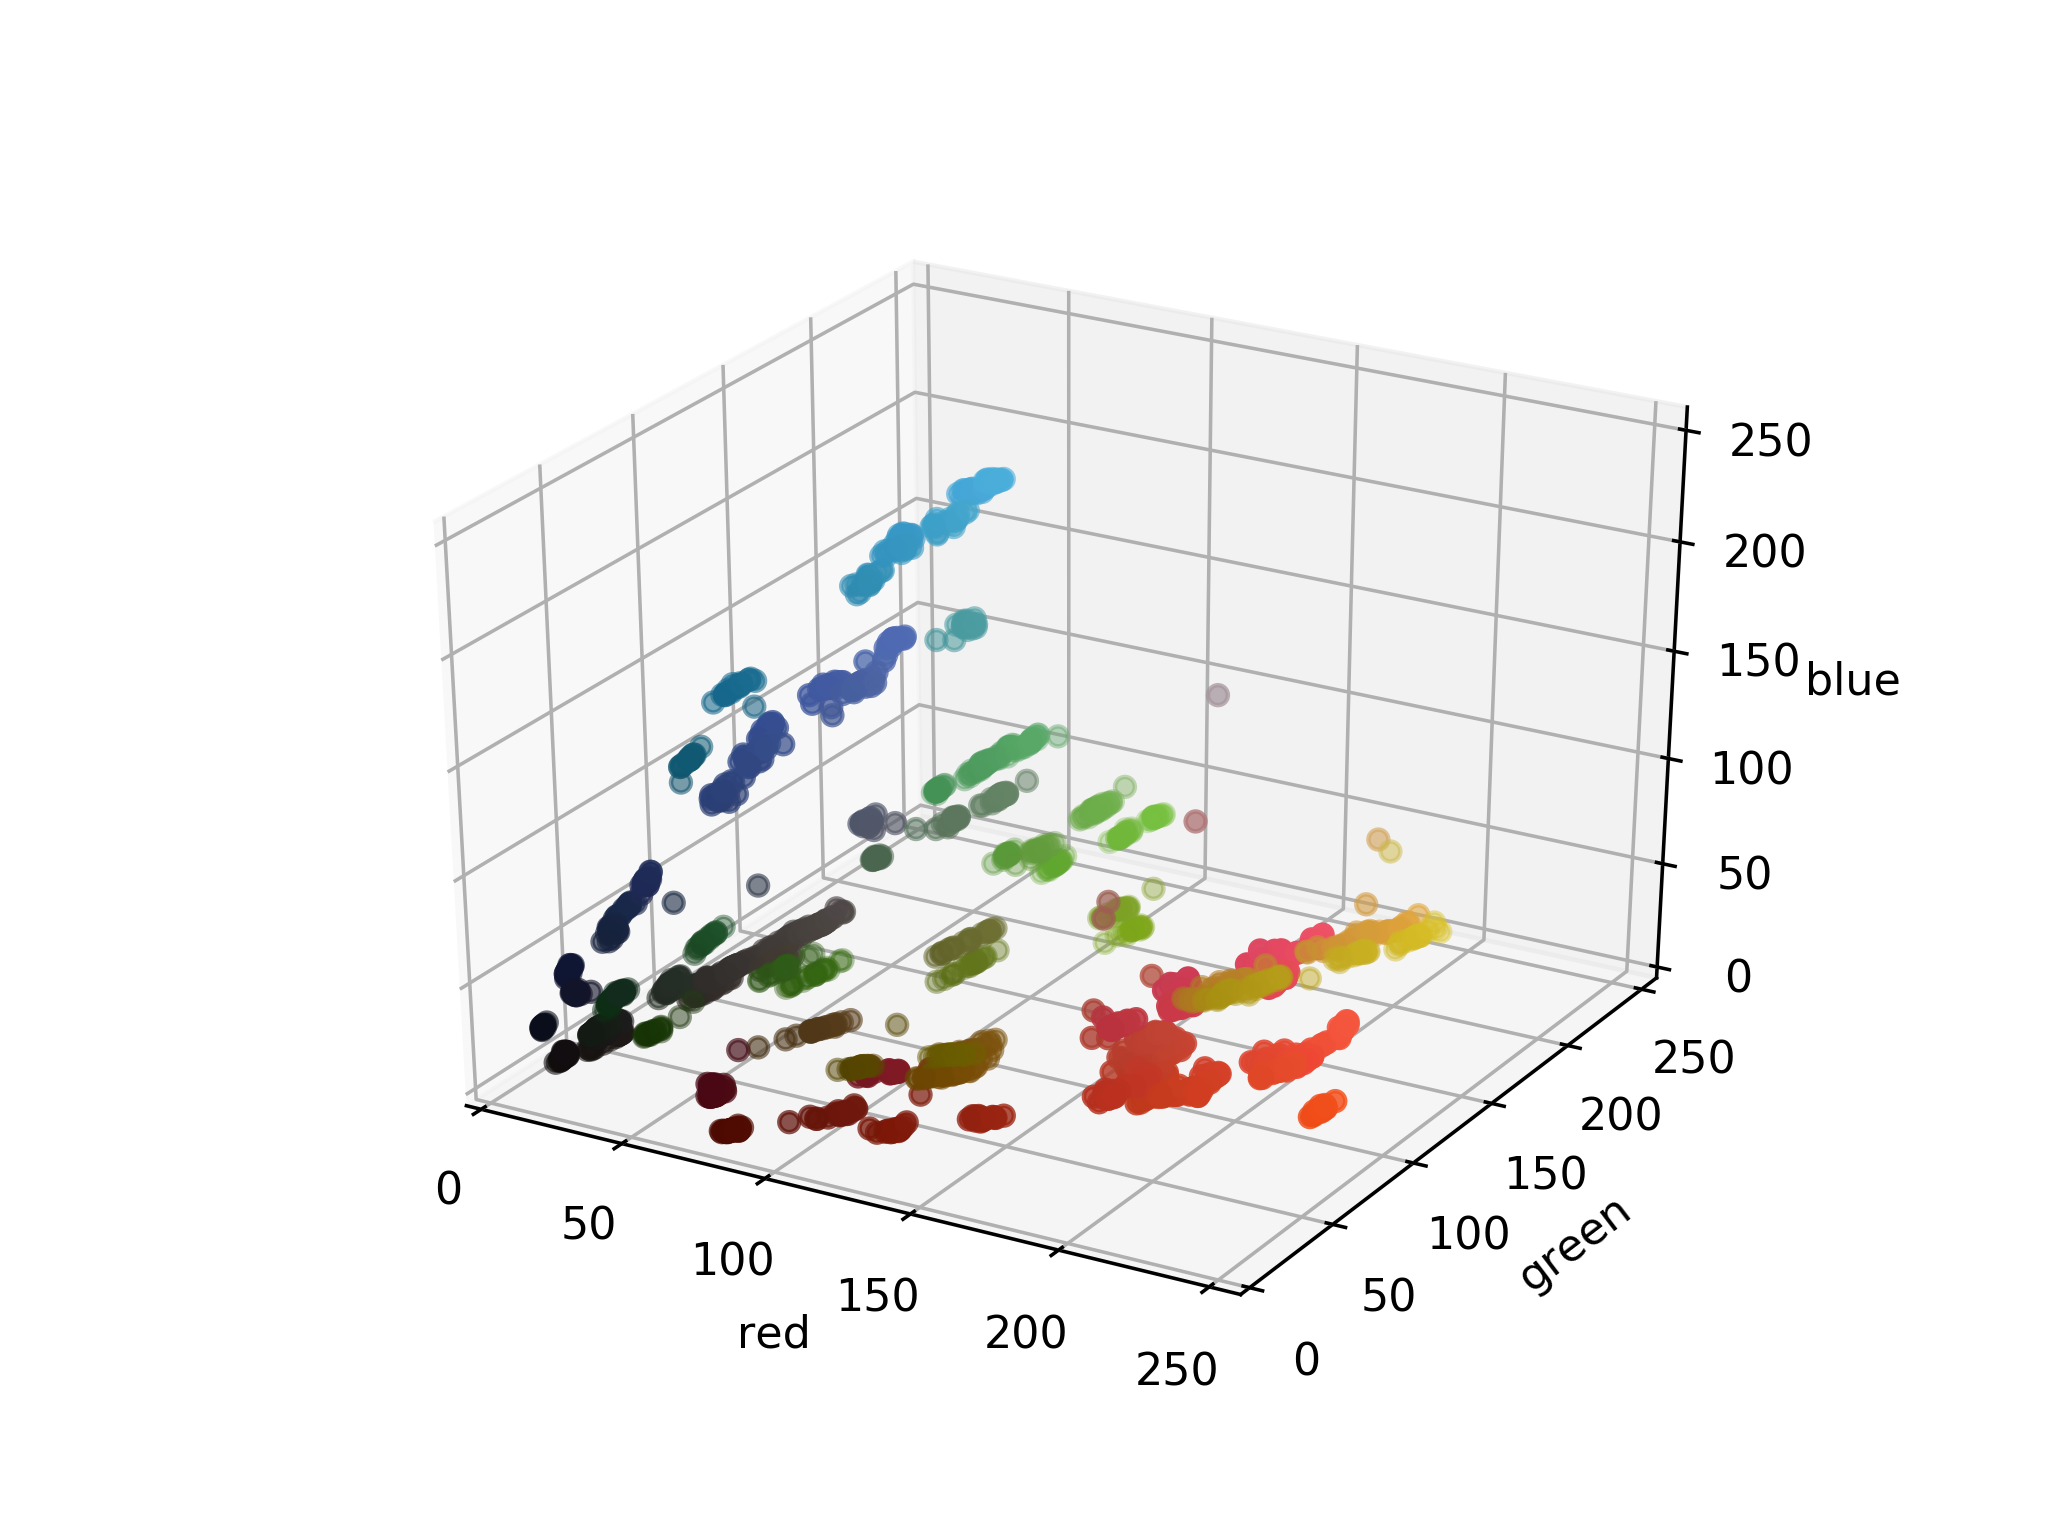
\includegraphics[width=\linewidth]{images/rgb.png}
				\caption{RGB colour space}
			\end{subfigure}
			\begin{subfigure}{.5\linewidth}
				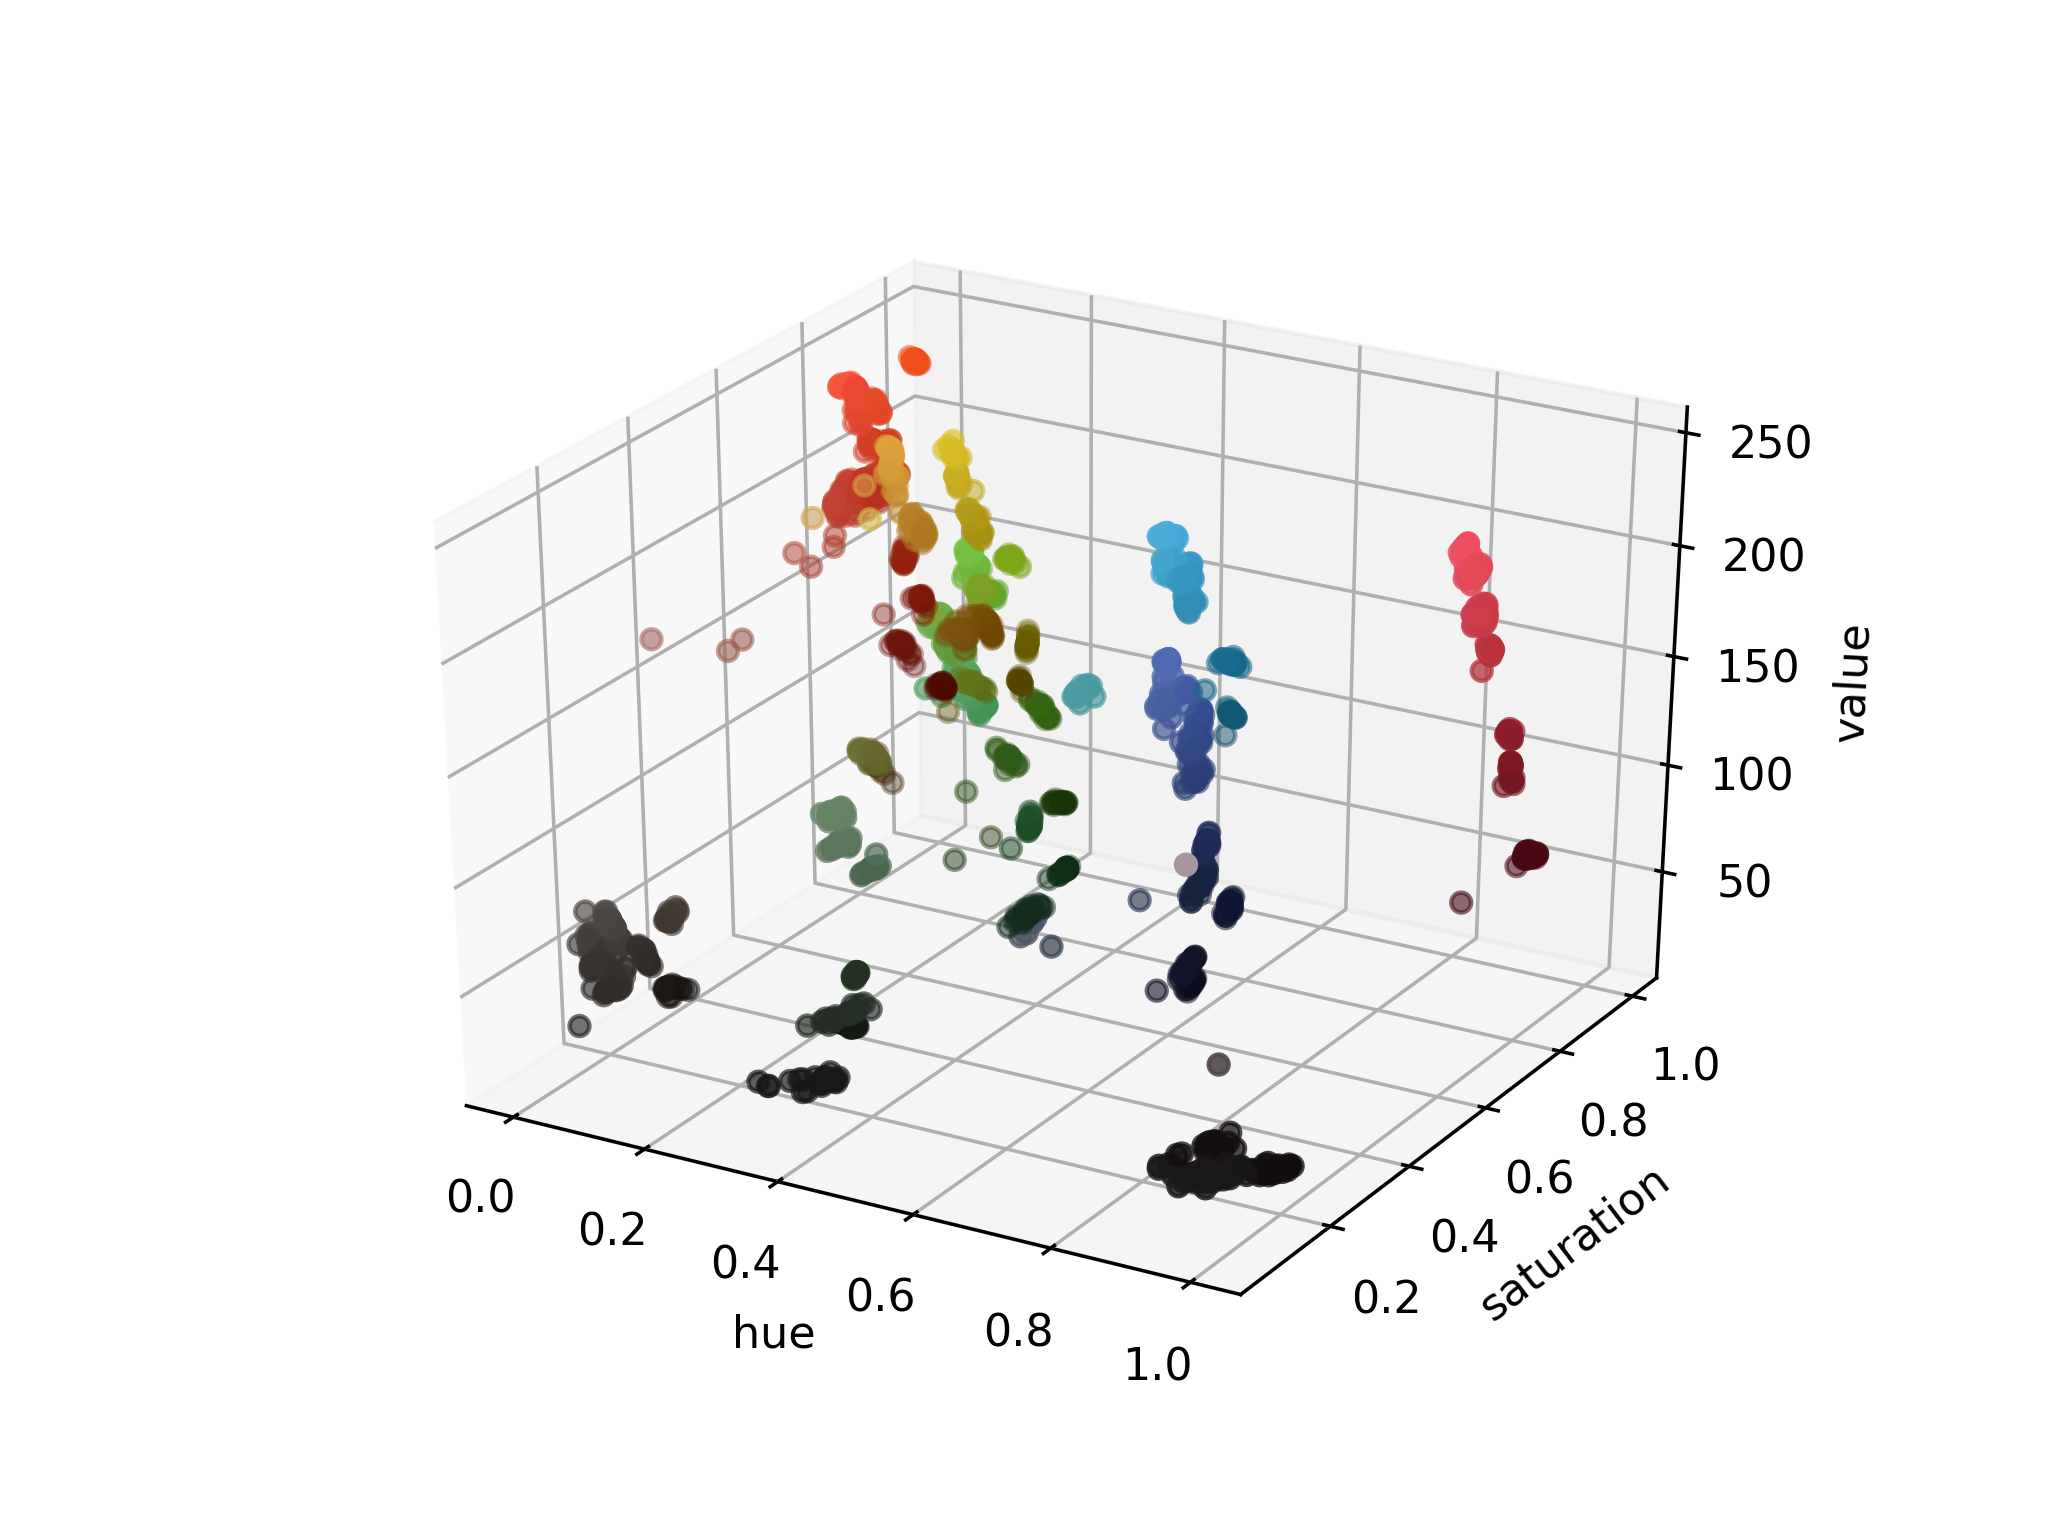
\includegraphics[width=\linewidth]{images/hsv.png}
				\caption{HSV colour space}
			\end{subfigure}
			\begin{subfigure}{.5\linewidth}
				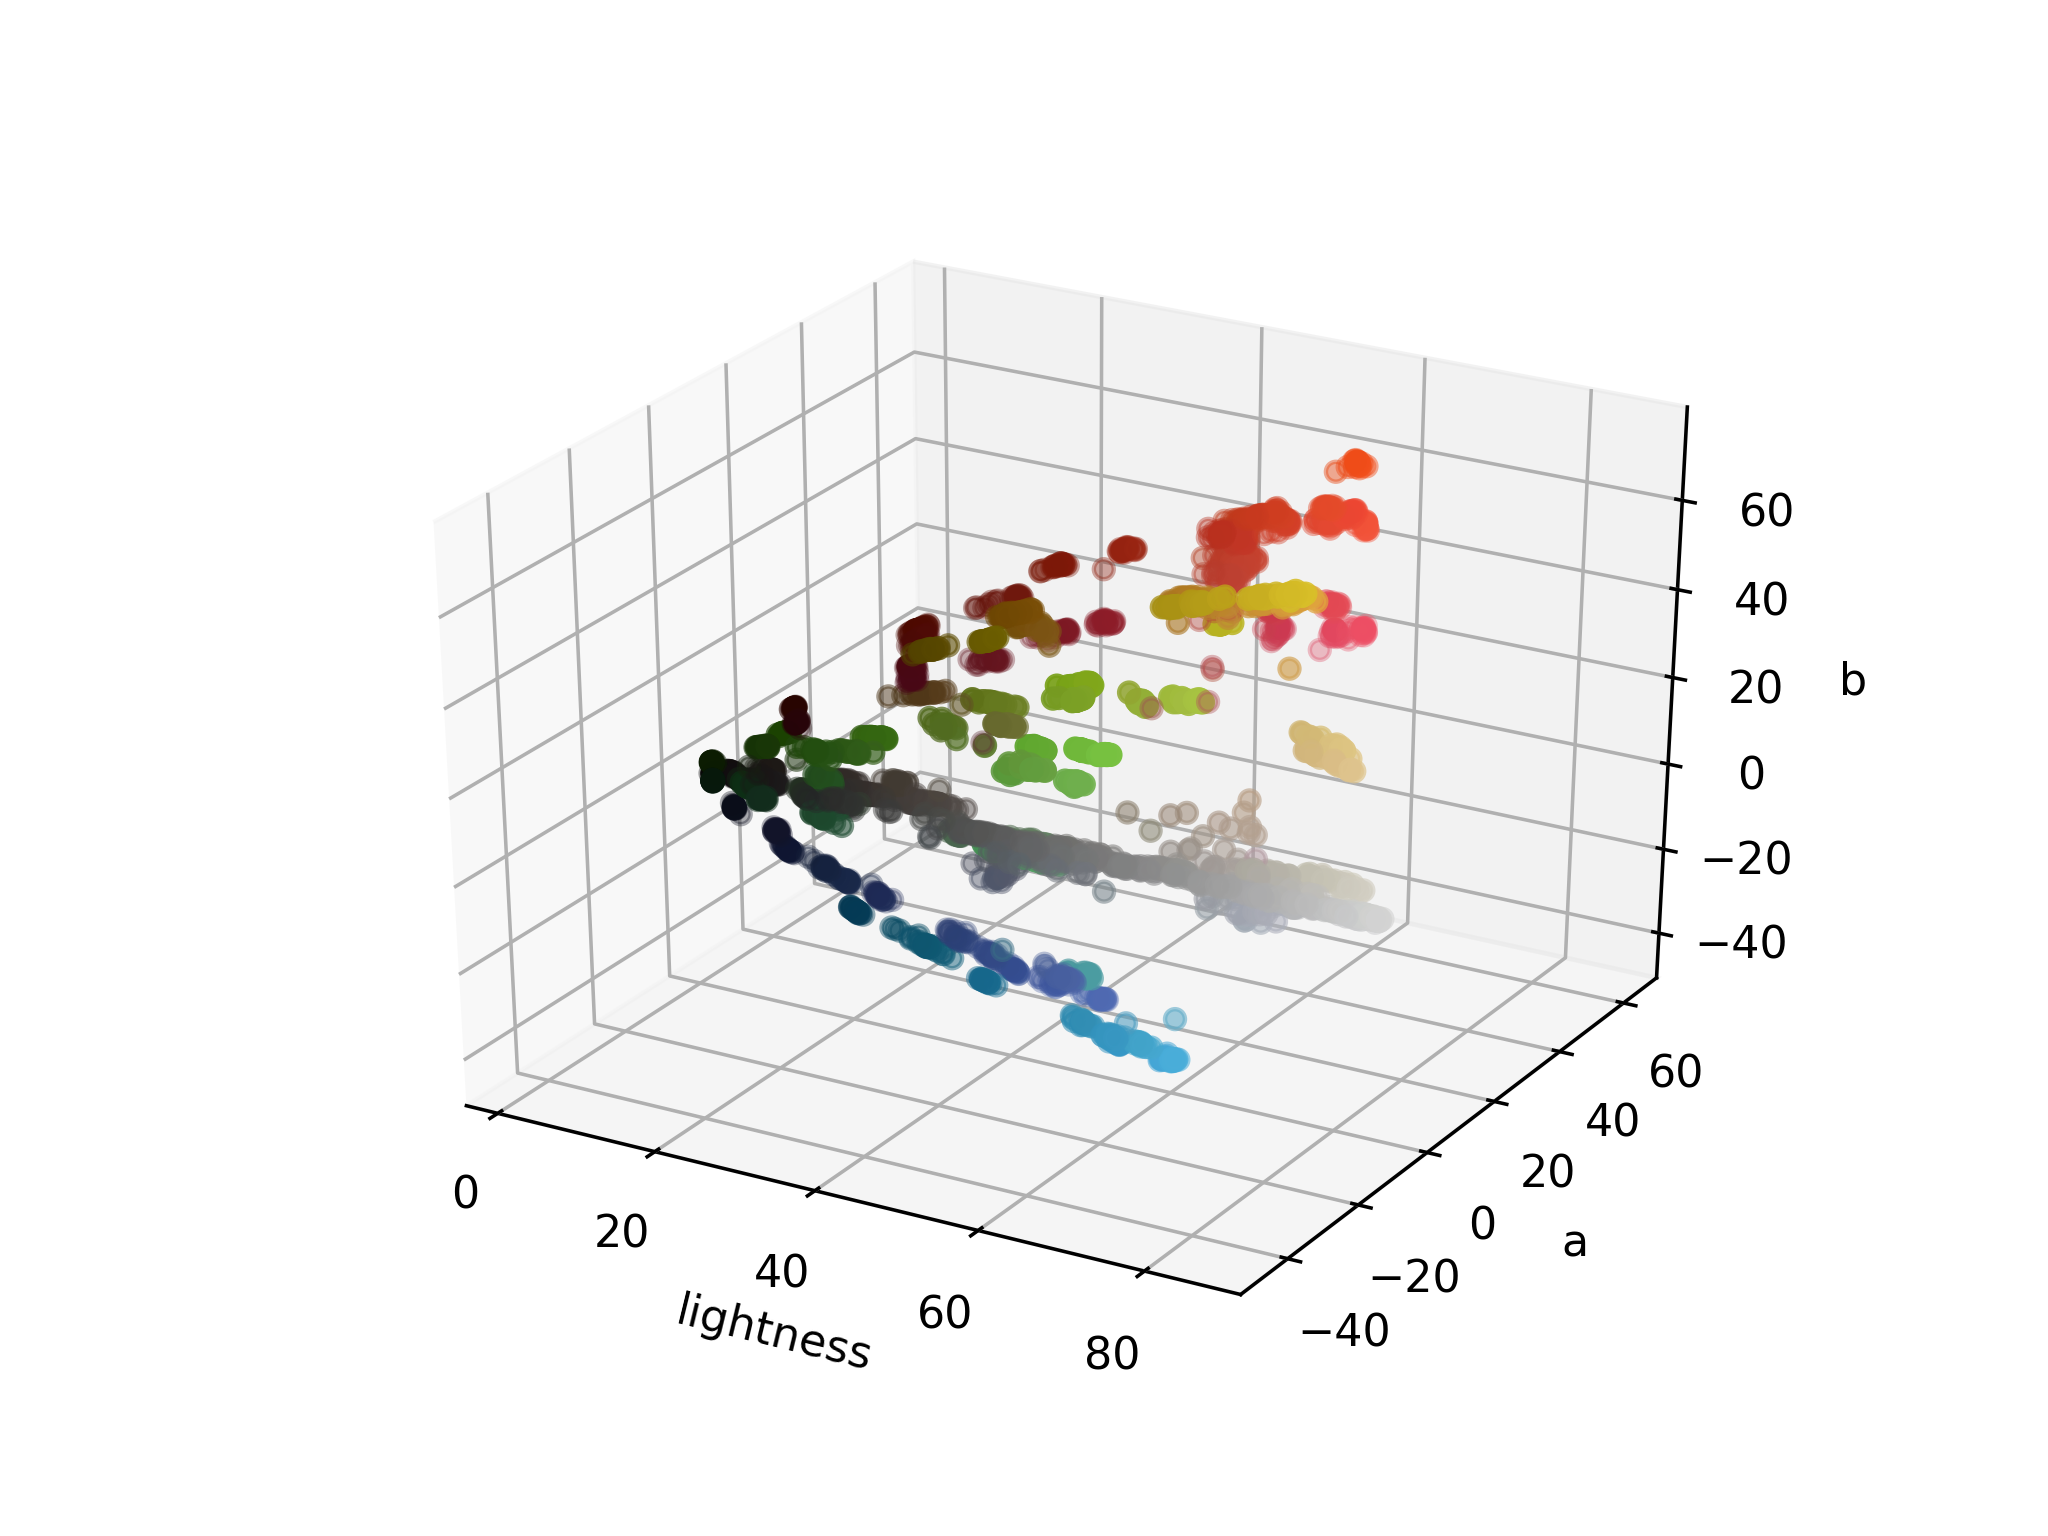
\includegraphics[width=\linewidth]{images/lab.png}
				\caption{CIELAB colour space}
			\end{subfigure}
			\caption{sampled colours, placed in different colour spaces}
		\end{figure}
	\end{center}

	To see the difference more clearly, we plotted below the same distributions as above except we displayed their colour labels (which colour the point was labeled as) instead of their actual colour.

	\begin{center}
		\begin{figure}[H]
			\begin{subfigure}{.5\linewidth}
				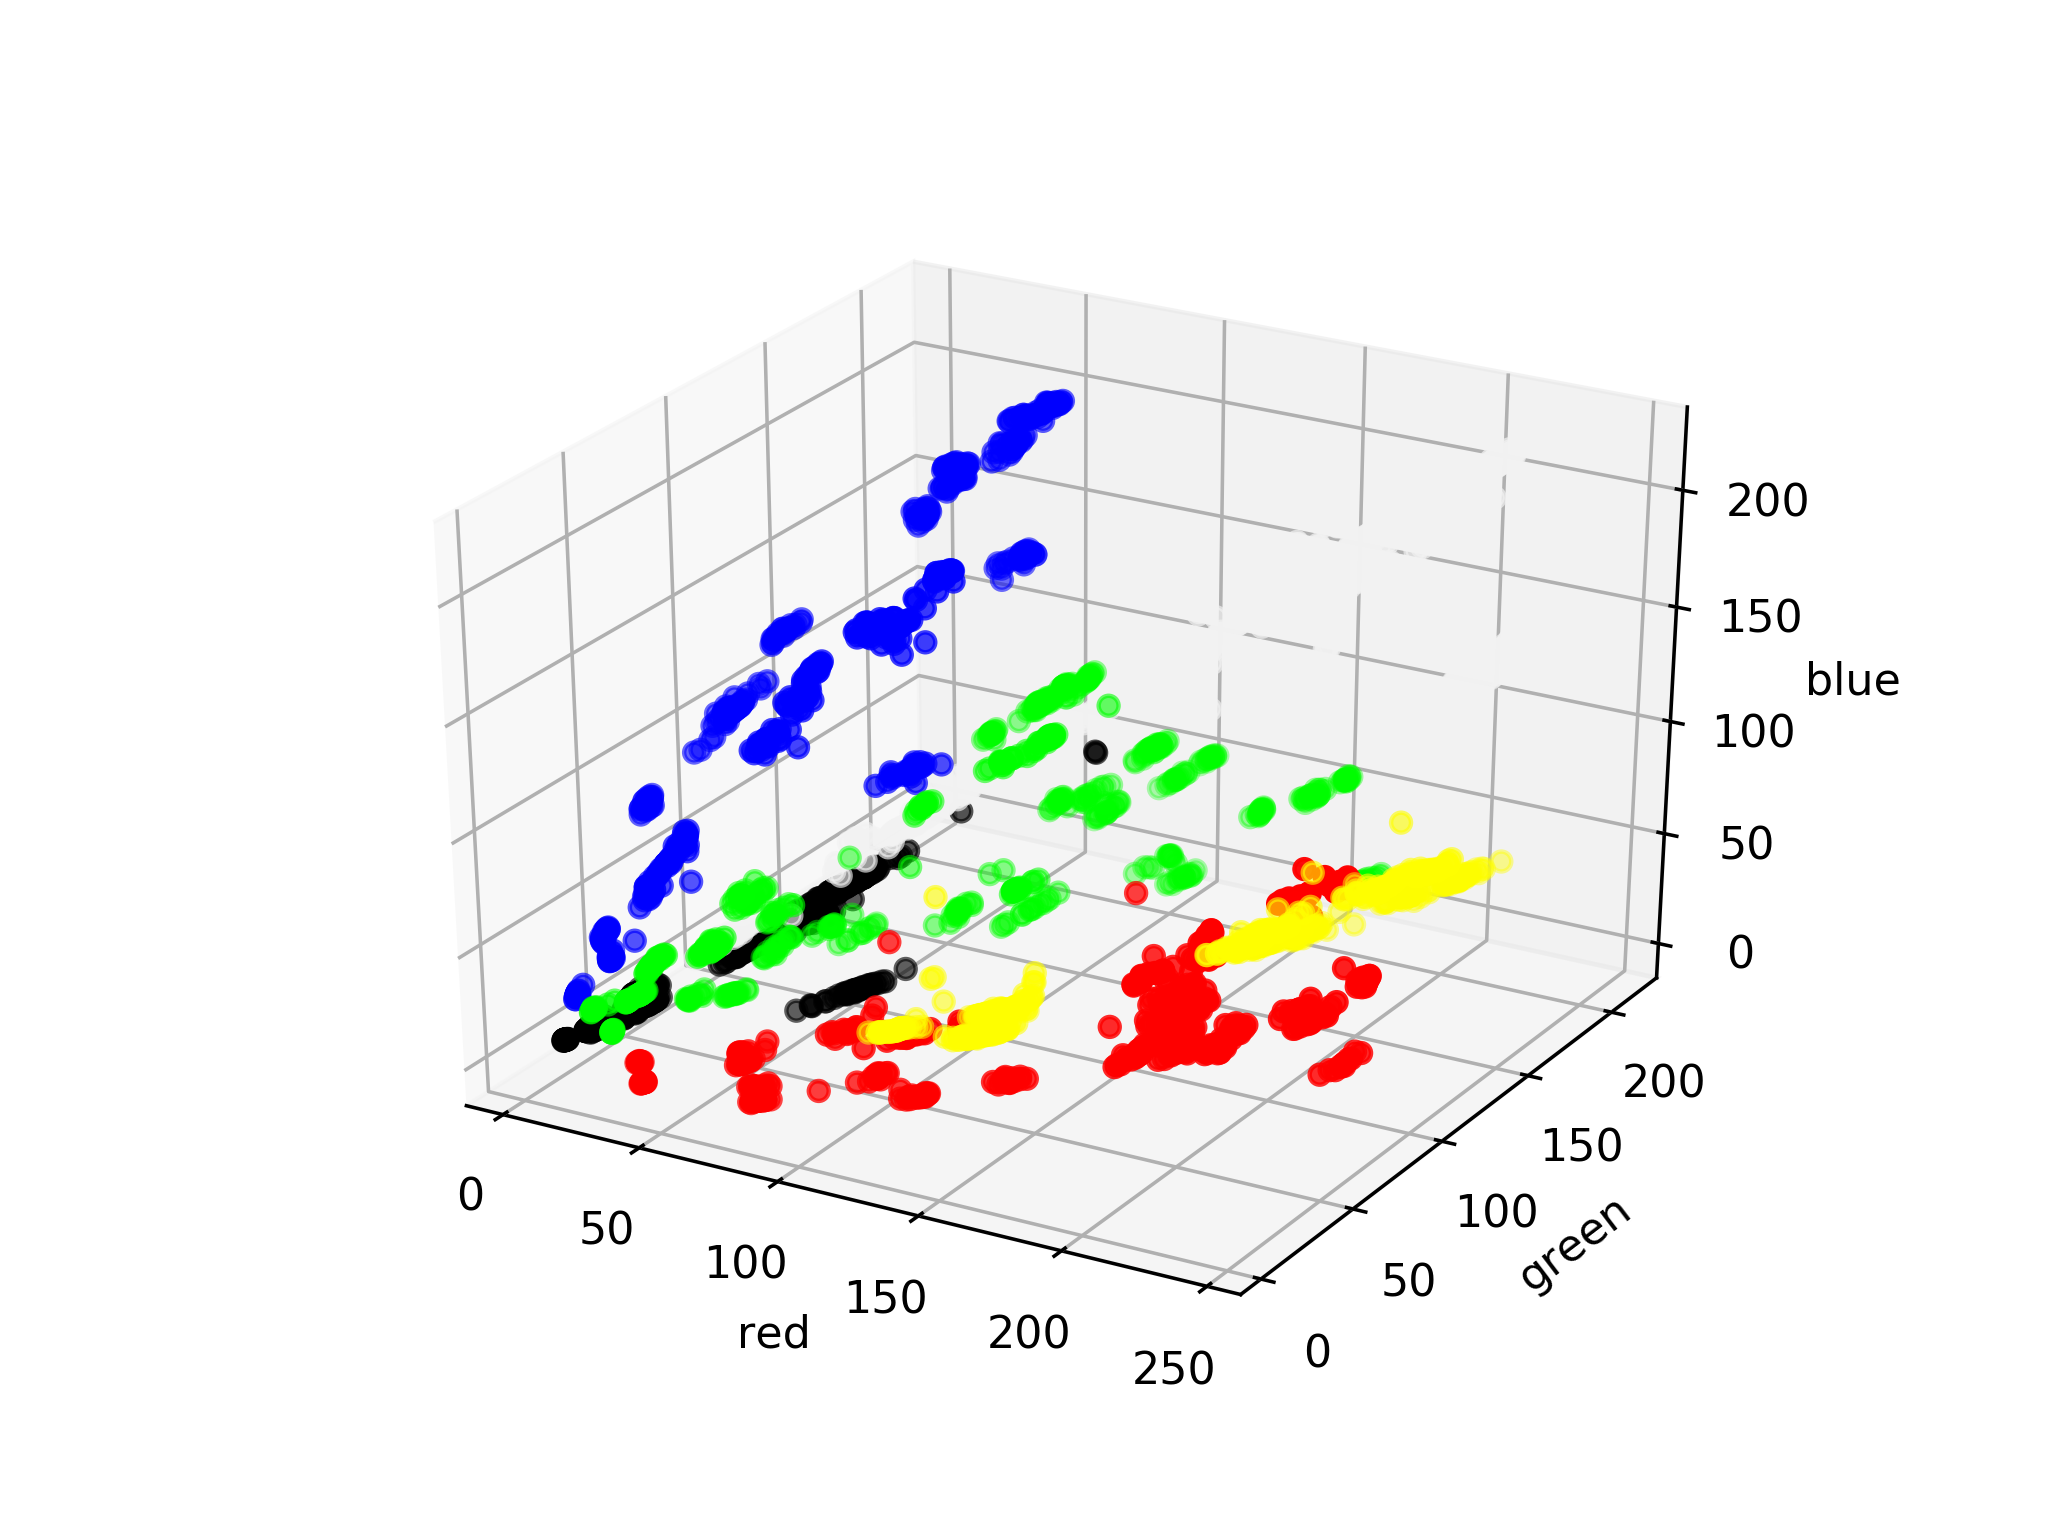
\includegraphics[width=\linewidth]{images/rgb_labels.png}
				\caption{RGB colour space}
			\end{subfigure}
			\begin{subfigure}{.5\linewidth}
				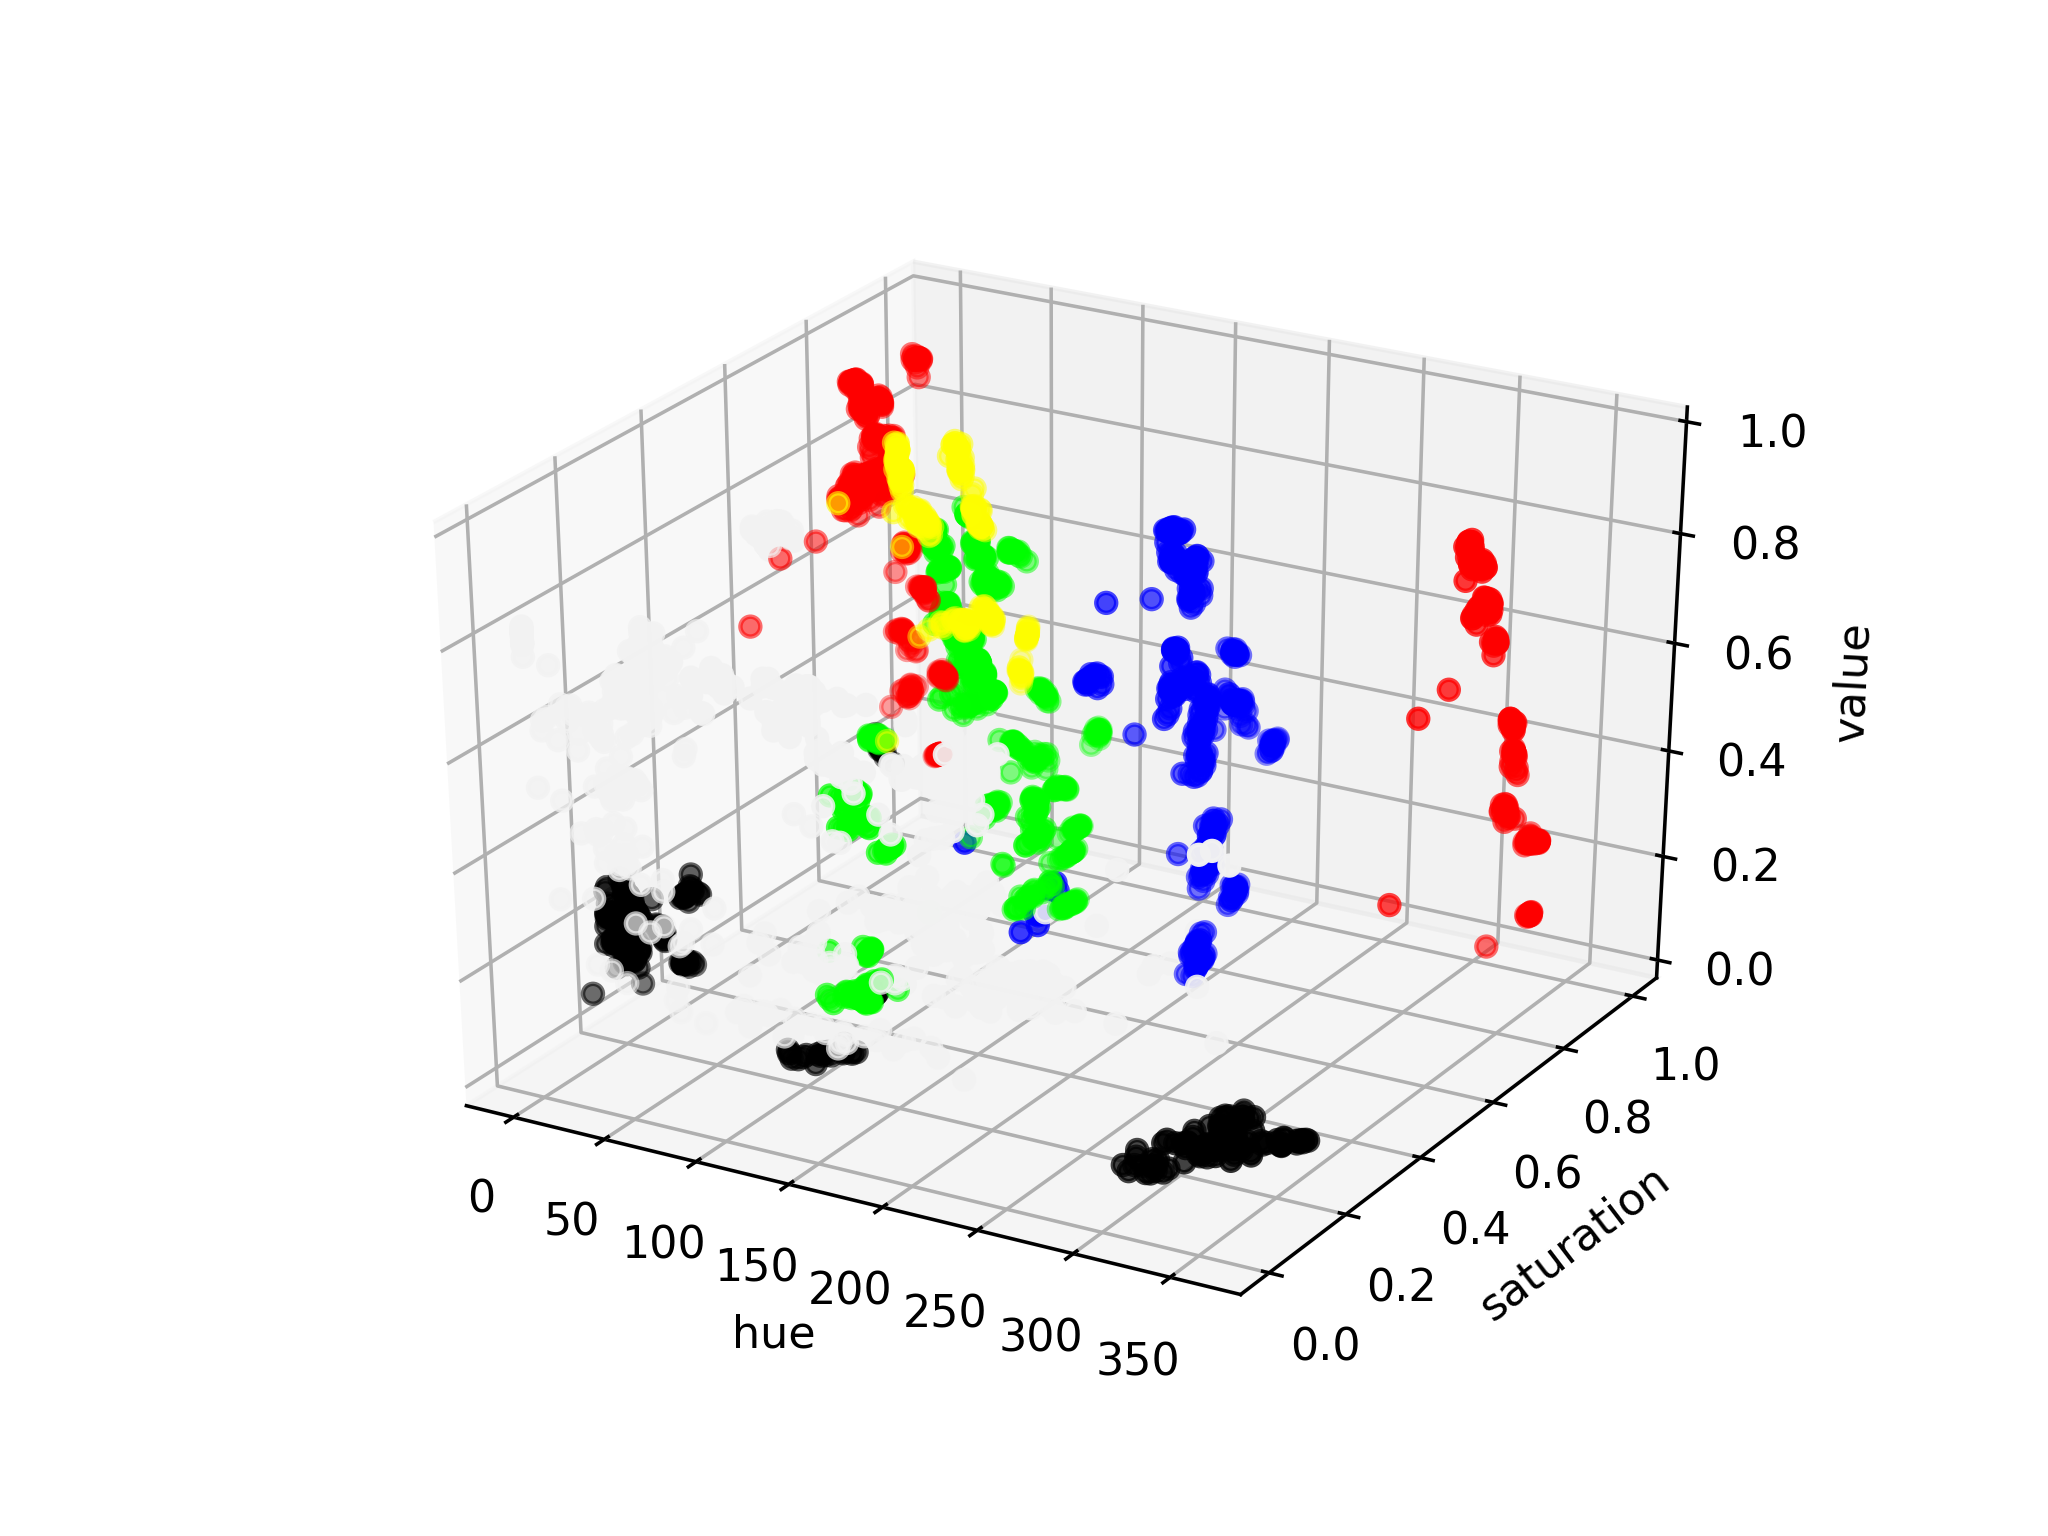
\includegraphics[width=\linewidth]{images/hsv_labels.png}
				\caption{HSV colour space}
			\end{subfigure}
			\begin{subfigure}{.5\linewidth}
				\centering
				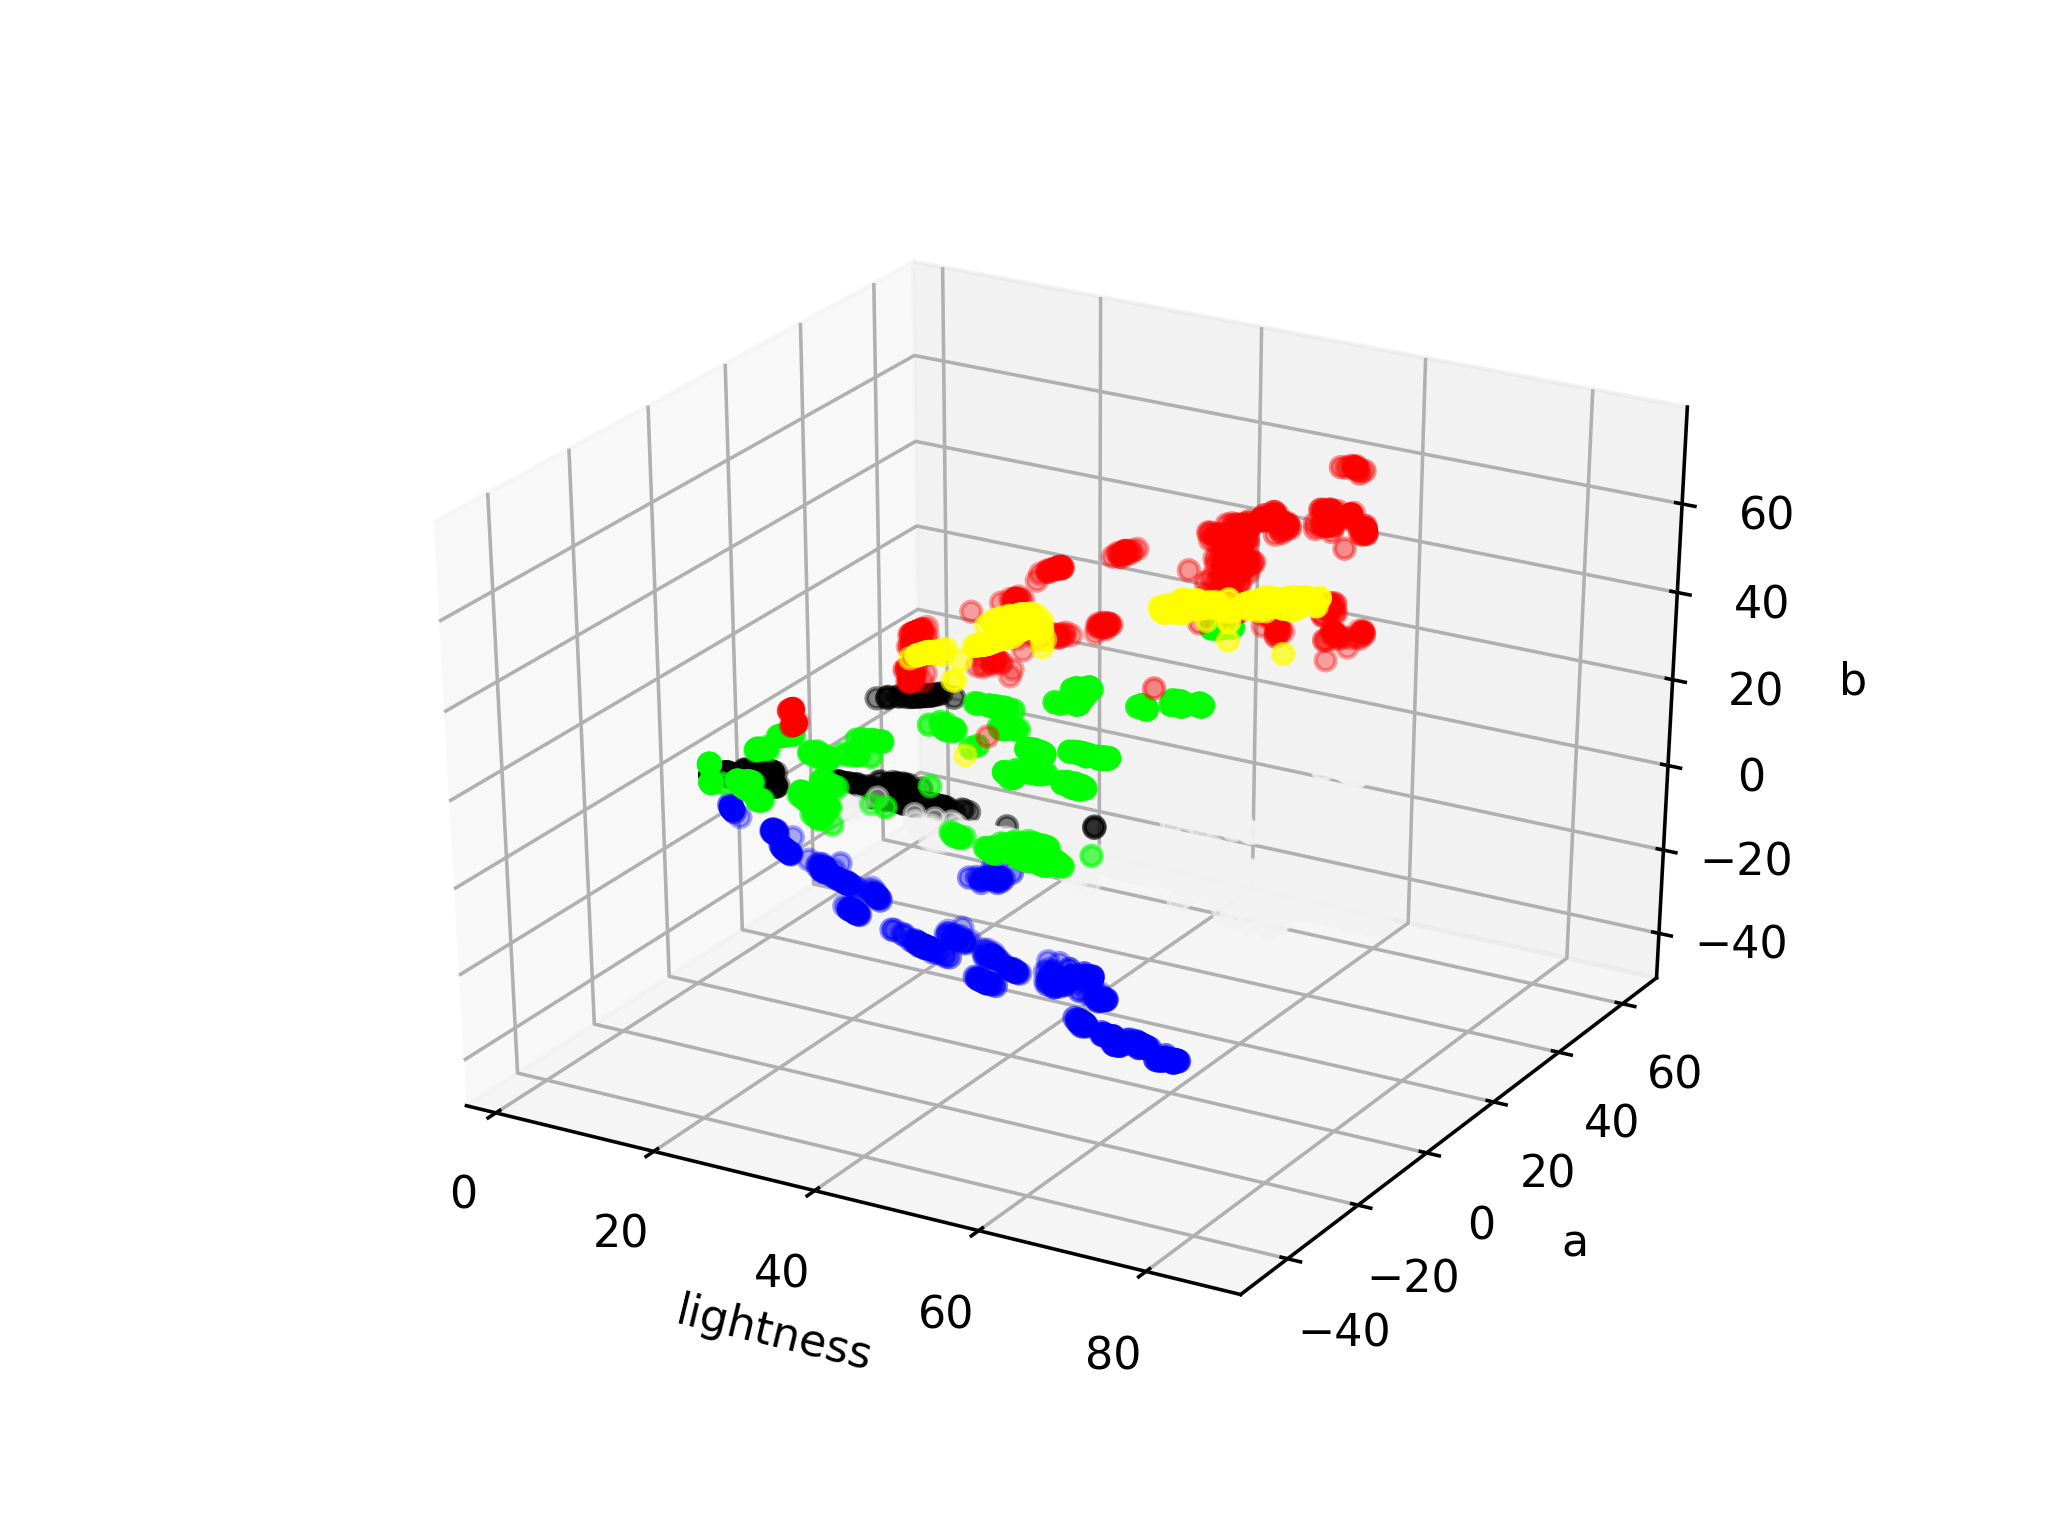
\includegraphics[width=\linewidth]{images/lab_labels.png}
				\caption{CIELAB colour space}
			\end{subfigure}
			\caption{labels of sampled colours, placed in different colour spaces}
		\end{figure}
	\end{center}
	
	The \texttt{RGB} and \texttt{HSV} are not natural colour spaces for humans. If two colours are close in \texttt{RGB} space (using euclidean distance), that doesn't mean that human perceive them as similar. There are some colour spaces that are more suited for human perception, for example the \texttt{CIELAB} colour space, also called \texttt{LAB}. \\

	\texttt{CIELAB} was designed so that the same amount of numerical change in these values corresponds to roughly the same amount of visually perceived change. The  \texttt{CIELAB} gamut includes both the gamuts of the \texttt{RGB} and \texttt{CYMK} colour models. It expresses colour as three values: $L^*$ for the lightness from black ($0$) to white ($100$), $a^*$ from green (-) to red ($+$), and $b^*$ from blue (-) to yellow ($+$). Because three parameters are measured, the space itself is a three-dimensional real number space, which allows for infinitely many possible colours. In practice, the space is usually mapped onto a three-dimensional integer space for digital representation, and thus the $L^*$, $a^*$, and $b^*$ values are usually absolute, with a pre-defined range. \\
	
	Since \texttt{LAB} is related to \texttt{RGB}, we can expect them to perform similarly.

	\section{Evaluating performance}

	We then tested different classifiers using training data set. Results can be found in the table below. Accuracy is measured using our testing set and is calculated for all three coulour spaces \texttt{RGB}, \texttt{HSV} and \texttt{LAB} colour space. When we trained our classifiers with points from circles, we tested with points from cylinders and vice versa. The best result for each classifier is displayed in \textbf{bold}.
	
	\begin{center}
		\begin{tabular}{|c|c|c|c||c|c|c|}
			\hline
			Training set & \multicolumn{3}{c||}{\textbf{Circles}} & \multicolumn{3}{c|}{\textbf{Cylinders}} \\
			\hline
			\hline 
			\textbf{Classifier} & \texttt{RGB} & \texttt{HSV} & \texttt{LAB} & \texttt{RGB} & \texttt{HSV} & \texttt{LAB} \\
			\hline \hline
			\textbf{knn}, \small k = 3 & 0.82 & 0.50 & 0.83 & 0.81 & 0.54 & \textbf{0.87} \\
			\textbf{knn}, \small k = 5 & 0.82 & 0.49 & 0.84 & 0.81 & 0.54 & \textbf{0.87} \\
			\textbf{knn}, \small k = 7 & 0.83 & 0.48 & 0.85 & 0.81 & 0.52 & \textbf{0.87} \\
			\hline \hline
			\textbf{decision tree}, \small gini & 0.75 & 0.80 & 0.78 & 0.70 & 0.84 & \textbf{0.88} \\
			\textbf{decision tree}, \small entropy & 0.76 & 0.74 & 0.78 & 0.74 & 0.83 & \textbf{0.88} \\
			\hline \hline
			\textbf{random forest}, \small gini & 0.79 & 0.78 & 0.82 & 0.78 & 0.78 & \textbf{0.89} \\
			\textbf{random forest}, \small entropy & 0.78 & 0.77 & 0.80 & 0.81 & 0.75 & \textbf{0.89} \\
			\hline \hline
			\textbf{naive bayes} & 0.75 & \textbf{0.92} & 0.91 & 0.72 & 0.70 & 0.84 \\
			\hline \hline
			\textbf{svm}, \small kernel=linear, c=0.025 & 0.85 & 0.72 & 0.86 & 0.89 & 0.60 & \textbf{0.90} \\
			\textbf{svm}, \small kernel=rbf, c=0.025 & 0.17 & \textbf{0.37} & 0.19 & 0.17 & 0.36 & 0.26 \\
			\textbf{svm}, \small kernel=linear, c=0.05 & 0.85 & 0.73 & 0.87 & 0.88 & 0.64 & \textbf{0.90} \\
			\textbf{svm}, \small kernel=linear, c=0.1 & 0.85 & 0.73 & 0.87 & 0.89 & 0.65 & \textbf{0.90} \\
			\textbf{svm}, \small kernel=linear, c=0.2 & 0.84 & 0.72 & 0.87 & 0.89 & 0.67 & \textbf{0.90} \\
			\hline
		\end{tabular} \\
	\end{center}

	% za k smo probali tudi utežene verzije ampak ker ni blo razlike, niso prikazani v tabeli.
	We also tried all knn versions from the table with added weights (distance). Since there was no noticable difference, we ommited it for better transparency of the results. \\

	We can see that parameters for support vector machine (svm) have some influence on the results. The most noticable difference is caused with a radial basis function (rbf) kernel instead of linear one. Kernels define the "shape" of the decision boundaries between classes. \\

	Linear kernel produces decision boundaries in the form of straight lines and rbf kernel is non-linear, which means it produces curved decision boundaries. This is also the reason why it has noticably better performance on the \texttt{HSV} - non-linear colour space. \\

	In a svm there is a tradeoff between finding a hyperplane with the largest minimum margin, and a hyperplane that correctly separates as many instances as possible. Parameter $c$ determines how much more we want the second thing from the tradeoff than the first one. Minimum margin determines the smallest distance at which the instance of the same class should be away from the decision boundary. \\
	
	Low c will therefore set a large minimum margin but won't put such an importance to also correctly classify the outliers, whereas large c will give more importace to have all the instances of a class, even the outliers, on the same side of the decision bounaries, which will consequently reduce the minimum margin and cause instances to be closer to the decision boundary. \\

	As we have predicted, in general the accuracy in \texttt{HSV} colour space is lower than that in the \texttt{RGB} space. As expected, \texttt{RGB} and \texttt{LAB} perform similarly, but the \texttt{LAB} performs slightly better. \\

	We can see that in most cases the best results are with \texttt{LAB} colour space and in the second scenario, where we trained our classifier with colours from cylinders and tested it with colours from the circles. Interestingly, the highest score of all classifiers is naive bayes on \texttt{HSV} colour space. \\

	%Overall, the best performing classifier is support vector machine, which is not suprising as our data consists of vectors.
	Since naive bayes showed the best performance, we wanted to understand it's performance better, so we looked at the confusion matrices of the top 2 results. \\

	\begin{center}
		\begin{tabular}{|c c c c c c c c|}
			\hline
			\multicolumn{1}{|c}{} & \multicolumn{6}{c}{\multirow{2}{*}{\textbf{\large naive bayes on \texttt{HSV}}}} & \multicolumn{1}{c|}{}\\
			\multicolumn{1}{|c}{} & & & & & & & \multicolumn{1}{c|}{}\\
			\hline
				& & \multicolumn{6}{|c|}{\textbf{predicted}} \\
				\multicolumn{2}{|c|}{}& \begin{sideways}red\end{sideways} & \begin{sideways}green\end{sideways} & \begin{sideways}blue\end{sideways} & \begin{sideways}yellow \end{sideways} & \begin{sideways}black\end{sideways} & \begin{sideways}white\end{sideways} \\ \hline
			\multirow{6}{*}{\begin{sideways}\textbf{actual}\end{sideways}}& \multicolumn{1}{c|}{red} &250 & 0 & 0 & 0 & 0 & 0 \\
			&\multicolumn{1}{c|}{green} & 31 & 209 & 3 & 0 & 5 & 2 \\
			&\multicolumn{1}{c|}{blue} & 10 & 0 & 240 & 0 & 0 & 0 \\
			&\multicolumn{1}{c|}{yellow} & 0 & 2 & 0 & 248 & 0 & 0 \\
			&\multicolumn{1}{c|}{black} & 0 & 0 & 0 & 0 & 198 & 52 \\
			&\multicolumn{1}{c|}{white} & 0 & 0 & 0 & 0 & 13 & 237 \\ \hline
		\end{tabular}
	\end{center}

	\begin{center}
		\begin{tabular}{|c c c c c c c c|}
			\hline
			\multicolumn{1}{|c}{} & \multicolumn{6}{c}{\multirow{2}{*}{\textbf{\large naive bayes on \texttt{LAB}}}} & \multicolumn{1}{c|}{}\\
			\multicolumn{1}{|c}{} & & & & & & & \multicolumn{1}{c|}{}\\
			\hline
				& & \multicolumn{6}{|c|}{\textbf{predicted}} \\
				\multicolumn{2}{|c|}{}& \begin{sideways}red\end{sideways} & \begin{sideways}green\end{sideways} & \begin{sideways}blue\end{sideways} & \begin{sideways}yellow \end{sideways} & \begin{sideways}black\end{sideways} & \begin{sideways}white\end{sideways} \\ \hline
			\multirow{6}{*}{\begin{sideways}\textbf{actual}\end{sideways}}& \multicolumn{1}{c|}{red} &250 & 0 & 0 & 0 & 0 & 0 \\
			&\multicolumn{1}{c|}{green} & 0 & 250 & 0 & 0 & 0 & 0 \\
			&\multicolumn{1}{c|}{blue} & 0 & 0 & 250 & 0 & 0 & 0 \\
			&\multicolumn{1}{c|}{yellow} & 0 & 1 & 0 & 249 & 0 & 0 \\
			&\multicolumn{1}{c|}{black} & 0 & 35 & 65 & 0 & 132 & 18 \\
			&\multicolumn{1}{c|}{white} & 0 & 1 & 8 & 0 & 4 & 237 \\ \hline
		\end{tabular}
	\end{center}

	Since these are multiclass confusion matrices, we read them a bit differently than the binary ones. This is explained in a picture below.

	\begin{figure}[H]
		\centering
		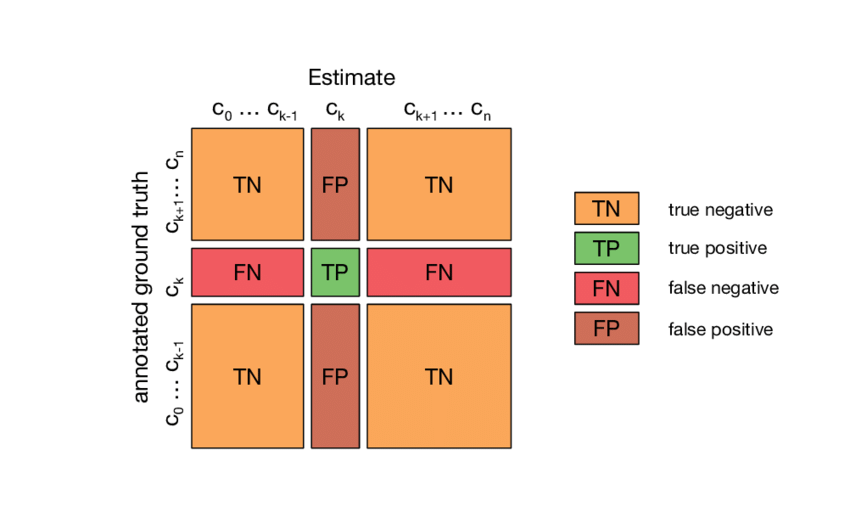
\includegraphics[width=1\linewidth]{images/Confusion_matrix_explanation.png}
		\caption{Multiclass confusion matrix, source: \small \textit{Activity, Context, and Plan Recognition with Computational Causal Behaviour Models - Scientific Figure on ResearchGate}}
	\end{figure}

	%https://www.researchgate.net/figure/Confusion-matrix-for-multi-class-classification-The-confusion-matrix-of-a_fig7_314116591

	We can see that on \texttt{HSV} colour space we have problems with confusing black and white, which happens beacuse white can appear as a dark grey sometimes. Some noticable confusion happens when classifier has to classify a green instance, which probably happens because one group of red instances lies really close to green ones in our graph of \texttt{HSV} colour space, see figure 5b. \\ 

	\texttt{LAB} colour space has no problems identifying red, green, blue and yellow but performs particularly bad on identifying black instances. We can explain mistaking black instances for green and blue ones with the fact that some of the green and blue instances are of quite dark shade. Confusion of black and white instances can be explained the same way as in \texttt{HSV} colour space. Black and white are two extremes of the grayscale and it's hard to correctly split it in two parts. \\

	\section{Conclusion}

	Based on the obtained results, we have two candidates to use with our robot. The first one is the one with the best score - naive bayes with \texttt{HSV}. The second one is naive bayes with \texttt{LAB}. \\ 
	
	Decision is though since naive bayes in combination with \texttt{LAB} colour space performs excellent for all except the black and white colours. In fact, \texttt{LAB} has a perfect score for identifying the first four colours. We expect those two colours to appear mainly in the environment and not as much in our objects of interest, rings and cylinders. With that assumption, the latter is definitely a better choice. \\

	The classifier we will use with our robot will be trained on both sets of images - circles and cylinders. This will make the classifier better as it will have a bigger spectrum of colours to learn from.\\
	
	As we can see from the table above, this type of classification works well. The only problem is that we have to choose points on our object, which can sometimes be problematic. But if we sample multiple points, the probability that our classification will be correct increases. \\

	Another approach which can robustify the classification is to take into accounts several frames that contain the object of interest, not just the current one. This also allows us to have a classifier that does not have a 100\% success rate.
	% uporabili bomo več zaporednih framov, zato ne potrebujemo 100% natančnosti
\end{document}